% Created 2015-01-28 Wed 23:13
\documentclass[12pt]{book}
\usepackage{graphicx}
\usepackage{xcolor}
\usepackage{xeCJK}
\setCJKmainfont{SimSun}
\usepackage{longtable}
\usepackage{float}
\usepackage{textcomp}
\usepackage{geometry}
\geometry{left=1.5cm,right=1.5cm,top=2cm,bottom=1.5cm}
\usepackage{multirow}
\usepackage{multicol}
\usepackage{listings}
\usepackage{algorithm}
\usepackage{algorithmic}
\usepackage{latexsym}
\usepackage{natbib}
\usepackage{fancyhdr}
\usepackage[xetex,colorlinks=true,CJKbookmarks=true,linkcolor=blue,urlcolor=blue,menucolor=blue]{hyperref}


\lstset{language=Java,numbers=left,numberstyle=\tiny,basicstyle=\ttfamily\small,tabsize=4,frame=none,escapeinside=``,extendedchars=false,keywordstyle=\color{blue!70},commentstyle=\color{red!55!green!55!blue!55!},rulesepcolor=\color{red!20!green!20!blue!20!}}
\author{deepwaterooo}
\date{\today}
\title{LeetCode Summary}
\hypersetup{
  pdfkeywords={},
  pdfsubject={},
  pdfcreator={Emacs 24.3.1 (Org mode 8.2.7c)}}
\begin{document}

\maketitle
\tableofcontents


\chapter{数组 Array}
\label{sec-1}
\section{Easy}
\label{sec-1-1}
\subsection{Remove Duplicates from Sorted Array}
\label{sec-1-1-1}
\subsection{Remove Element}
\label{sec-1-1-2}
\subsection{Plus One}
\label{sec-1-1-3}
\section{Medium}
\label{sec-1-2}
\subsection{Rotate Image}
\label{sec-1-2-1}
\subsection{Set Matrix Zeroes}
\label{sec-1-2-2}
\subsection{Remove Duplicates from Sorted Array II}
\label{sec-1-2-3}
\subsection{Search in Rotated Sorted Array II}
\label{sec-1-2-4}
\subsection{3Sum}
\label{sec-1-2-5}
\subsection{3Sum Closest}
\label{sec-1-2-6}
\subsection{4Sum}
\label{sec-1-2-7}
\subsection{Remove Element}
\label{sec-1-2-8}
\subsection{Next Permutation}
\label{sec-1-2-9}
\subsection{Permutation Sequence}
\label{sec-1-2-10}
\subsection{Valid Sudoku}
\label{sec-1-2-11}
\subsection{Trapping Rain Water}
\label{sec-1-2-12}
\subsection{Gray Code}
\label{sec-1-2-13}
\section{Hard}
\label{sec-1-3}
\subsection{Search in Rotated Sorted Array}
\label{sec-1-3-1}
\subsection{Median of Two Sorted Arrays}
\label{sec-1-3-2}
\subsection{Longest Consecutive Sequence}
\label{sec-1-3-3}
\subsection{Trapping Rain Water}
\label{sec-1-3-4}
\section{others Covered}
\label{sec-1-4}
\begin{itemize}
\item Construct Binary Tree from Inorder and Postorder Traversal
\ref{sec-4-2-2}
\item Construct Binary Tree from Preorder and Inorder Traversal
\ref{sec-4-2-1}
\item Best Time to Buy and Sell Stock
\ref{sec-13-1-2}
\item Best Time to Buy and Sell Stock II        
\ref{sec-13-1-3}
\item Largest Rectangle in Histogram
\ref{sec-5-3-3}
\item Maximal Rectangle
\texttt{Maximum Rectangle}
\item Pascal's Triangle
\item Pascal's Triangle II
\item Merge Sorted Array        
\ref{sec-7-1-1}
\item Two Sum
\ref{sec-6-2-1}
\item Two Sum II - Input array is sorted
\ref{sec-15-2-6}
\item Spiral Matrix
\ref{sec-20-1-7}
\item Spiral Matrix II
\ref{sec-20-1-8}
\item Sort Colors
\ref{sec-7-2-1}
\item Insert Interval
\ref{sec-20-1-5}
\item Merge Intervals
\ref{sec-20-1-6}
\end{itemize}
\subsection{Majority Element}
\label{sec-1-4-1}
\subsection{Container With Most Water}
\label{sec-1-4-2}
\subsection{Minimum Path Sum}
\label{sec-1-4-3}
\begin{itemize}
\item Search Insert Position
\ref{sec-8-1-2}
\item Unique Paths
\item Search for a Range
\ref{sec-8-1-1}
\item Search a 2D Matrix
\ref{sec-8-1-3}
\item Unique Paths II
\end{itemize}
\subsection{Missing Ranges}
\label{sec-1-4-4}
\subsection{Find Minimum in Rotated Sorted Array}
\label{sec-1-4-5}
\subsection{Triangle}
\label{sec-1-4-6}
\begin{itemize}
\item Maximum Subarray
\texttt{Maximum Subarray}
\item Maximum Product Subarray
\ref{sec-14-2-7}
\item Word Search
\ref{sec-11-2-4}
\item Combination Sum        
\ref{sec-11-1-4}
\item Combination Sum II
\ref{sec-11-1-5}
\item Subsets
\ref{sec-9-1-1}
\item Subsets II
\ref{sec-9-1-2}
\item Jump Game
\ref{sec-13-1-4}
\end{itemize}
\subsection{Find Peak Element}
\label{sec-1-4-7}
\subsection{Find Minimum in Rotated Sorted Array II}
\label{sec-1-4-8}
\subsection{Jump Game II}
\label{sec-1-4-9}
\begin{itemize}
\item First Missing Positive        
\ref{sec-7-3-3}
\item Word Ladder II
\end{itemize}
\ref{sec-10-2-1}
\begin{itemize}
\item Best Time to Buy and Sell Stock III
\ref{sec-14-3-1}
\item Roman to Integers
\texttt{Roman to Integers}
\item Integer to Roman
\ref{sec-2-2-2}
\item Pow(x, n)
\ref{sec-12-1-1}
\item Sqrt(x)
\ref{sec-12-1-2}
\end{itemize}

\chapter{字符串 String}
\label{sec-2}
\section{Easy}
\label{sec-2-1}
\subsection{Valid Palindrome}
\label{sec-2-1-1}
\subsection{Implement strStr()}
\label{sec-2-1-2}
\subsection{String to Integer (atoi)}
\label{sec-2-1-3}
\subsection{Add Binary}
\label{sec-2-1-4}
\subsection{Longest Common Prefix}
\label{sec-2-1-5}
\subsection{Roman to Integer}
\label{sec-2-1-6}
\subsection{Count and Say}
\label{sec-2-1-7}
\subsection{Length of Last Word}
\label{sec-2-1-8}
\section{Medium}
\label{sec-2-2}
\subsection{Longest Palindromic Substring}
\label{sec-2-2-1}
\subsection{Integer to Roman}
\label{sec-2-2-2}
\subsection{Anagrams}
\label{sec-2-2-3}
\subsection{Simplify Path}
\label{sec-2-2-4}
\section{Hard}
\label{sec-2-3}
\subsection{Valid Number}
\label{sec-2-3-1}
\subsection{Edit Distance}
\label{sec-2-3-2}
\subsection{Minimum Window Substring}
\label{sec-2-3-3}
\subsection{Longest Substring with At Most Two Distinct Characters}
\label{sec-2-3-4}
\subsection{Read N Characters Given Read4 II - Call multiple times}
\label{sec-2-3-5}
\section{other Covered}
\label{sec-2-4}
\begin{itemize}
\item Longest Valid Parentheses
\ref{sec-5-3-1}
\end{itemize}
\subsection{Valid Parentheses}
\label{sec-2-4-1}
\subsection{Compare Version Numbers}
\label{sec-2-4-2}
\subsection{Read N Characters Given Read4}
\label{sec-2-4-3}
\subsection{One Edit Distance}
\label{sec-2-4-4}
\subsection{Decode Ways}
\label{sec-2-4-5}
\subsection{Longest Substring Without Repeating Characters}
\label{sec-2-4-6}
\subsection{Reverse Words in a String}
\label{sec-2-4-7}
\subsection{Interleaving String}
\label{sec-2-4-8}

\begin{itemize}
\item Multiply Strings
\item Substring with Concatenation of All Words
\item ZigZag Conversion
\item Text Justification
\item Restore IP Addresses

\item Letter Combinations of a Phone Number
\item Generate Parentheses
\item Regular Expression Matching
\item Wildcard Matching
\item Scramble String
\item Distinct Subsequences
\item Word Ladder II \ref{sec-10-2-1}
\end{itemize}
\chapter{Linked List}
\label{sec-3}
\section{Easy}
\label{sec-3-1}
\subsection{Remove Duplicates from Sorted List}
\label{sec-3-1-1}
\subsection{Remove Nth Node From End of List}
\label{sec-3-1-2}
\subsection{Merge Two Sorted Lists}
\label{sec-3-1-3}
\subsection{Intersection of Two Linked Lists}
\label{sec-3-1-4}
\section{Medium}
\label{sec-3-2}
\subsection{Add Two Numbers}
\label{sec-3-2-1}
\subsection{Reverse Linked List II}
\label{sec-3-2-2}
\subsection{Partition List}
\label{sec-3-2-3}
\subsection{Remove Duplicates from Sorted List II}
\label{sec-3-2-4}
\subsection{Rotate List}
\label{sec-3-2-5}
\subsection{Swap Nodes in Pairs}
\label{sec-3-2-6}
\subsection{Reorder List}
\label{sec-3-2-7}
\subsection{Convert Sorted List to Binary Search Tree}
\label{sec-3-2-8}
\subsection{Linked List Cycle}
\label{sec-3-2-9}
\subsection{Linked List Cycle II}
\label{sec-3-2-10}
\section{Hard}
\label{sec-3-3}
\subsection{Reverse Nodes in k-Group}
\label{sec-3-3-1}
\subsection{Copy List with Random Pointer}
\label{sec-3-3-2}
\section{other Covered}
\label{sec-3-4}
\begin{itemize}
\item Sort List
\ref{sec-7-2-2}
\item Insertion Sort List
\ref{sec-7-3-2}
\item Merge k Sorted Lists
\texttt{Merge k Sorted Lists}
\end{itemize}
\chapter{树 Binary Tree, Binary Search Tree}
\label{sec-4}
\section{二叉树的遍历}
\label{sec-4-1}

树的遍历有两类:深度优先遍历和宽度优先遍历。深度优先遍历又可分为两种:先根(次序)遍历和后根(次序)遍历。

树的先根遍历是:先访问树的根结点,然后依次先根遍历根的各棵子树。树的先跟遍历的结果与对应二叉树(孩子兄弟表示法)的先序遍历的结果相同。

树的后根遍历是:先依次后根遍历树根的各棵子树,然后访问根结点。树的后跟遍历的结果与对应二叉树的中序遍历的结果相同。

二叉树的先根遍历有: 先序遍历 (root -> left -> right), root -> right -> left; 后根遍历有: 后序遍历(left -> right -> root), right -> left -> root; 二叉树还有个一般的树没有的遍历次序, 中序遍历 (left -> root -> right)。

\subsection{Binary Tree Preorder Traversal}
\label{sec-4-1-1}
Given a binary tree, return the preorder traversal of its nodes' values.

For example:

Given binary tree \{1,\#,2,3\},
\lstset{language=java,label= ,caption= ,numbers=none}
\begin{lstlisting}
1
 \
  2
 /
3
\end{lstlisting}

return [1,2,3].

Note: Recursive solution is trivial, could you do it iteratively?

用栈或Morris遍历
\begin{enumerate}
\item 栈: 使用栈,时间复杂度 O(n), 空间复杂度 O(n)
\label{sec-4-1-1-1}
\item Morris先序遍历: Morris 先序遍历,时间复杂度 O(n),空间复杂度 O(1)
\label{sec-4-1-1-2}
\end{enumerate}

\subsection{Binary Tree Inorder Traversal}
\label{sec-4-1-2}
Given a binary tree, return the inorder traversal of its nodes' values.

For example:

Given binary tree \{1,\#,2,3\},
\lstset{language=java,label= ,caption= ,numbers=none}
\begin{lstlisting}
1
 \
  2
 /
3
\end{lstlisting}

return [1,3,2].

Note: Recursive solution is trivial, could you do it iteratively?
\begin{enumerate}
\item 栈: 使用栈,时间复杂度 O(n), 空间复杂度 O(n)
\label{sec-4-1-2-1}
\item Morris先序遍历: Morris 先序遍历,时间复杂度 O(n),空间复杂度 O(1)
\label{sec-4-1-2-2}
\end{enumerate}


\subsection{Binary Tree Postorder Traversal}
\label{sec-4-1-3}
Given a binary tree, return the postorder traversal of its nodes' values.

For example:

Given binary tree \{1,\#,2,3\},
\lstset{language=java,label= ,caption= ,numbers=none}
\begin{lstlisting}
1
 \
  2
 /
3
\end{lstlisting}

return [3,2,1].

Note: Recursive solution is trivial, could you do it iteratively?
\begin{enumerate}
\item 栈: 使用栈,时间复杂度 O(n), 空间复杂度 O(n)
\label{sec-4-1-3-1}
\item Morris先序遍历: Morris 先序遍历,时间复杂度 O(n),空间复杂度 O(1)
\label{sec-4-1-3-2}
\end{enumerate}


\subsection{Binary Tree Level Order Traversal}
\label{sec-4-1-4}
Given a binary tree, return the level order traversal of its nodes' values. (ie, from left to right, level by level).

For example:

Given binary tree \{3,9,20,\#,\#,15,7\},
\lstset{language=java,label= ,caption= ,numbers=none}
\begin{lstlisting}
  3
 / \
9  20
  /  \
 15   7
\end{lstlisting}
return its level order traversal as:
\lstset{language=java,label= ,caption= ,numbers=none}
\begin{lstlisting}
[
  [3],
  [9,20],
  [15,7]
]
\end{lstlisting}
\begin{enumerate}
\item 递归版
\label{sec-4-1-4-1}
\item 迭代版
\label{sec-4-1-4-2}
\end{enumerate}

\subsection{Binary Tree Level Order Traversal II}
\label{sec-4-1-5}
Given a binary tree, return the bottom-up level order traversal of its nodes' values. (ie, from left to right, level by level from leaf to root).

For example:
Given binary tree \{3,9,20,\#,\#,15,7\},
\lstset{language=java,label= ,caption= ,numbers=none}
\begin{lstlisting}
  3
 / \
9  20
  /  \
 15   7
\end{lstlisting}
return its bottom-up level order traversal as:
\lstset{language=java,label= ,caption= ,numbers=none}
\begin{lstlisting}
[
  [15,7],
  [9,20],
  [3]
]
\end{lstlisting}
\begin{enumerate}
\item 递归版
\label{sec-4-1-5-1}
\item 迭代版
\label{sec-4-1-5-2}
\end{enumerate}


\subsection{Binary Tree Zigzag Level Order Traversal}
\label{sec-4-1-6}
Given a binary tree, return the zigzag level order traversal of its nodes' values. (ie, from left to right, then right to left for the next level and alternate between).

For example:

Given binary tree \{3,9,20,\#,\#,15,7\},
\lstset{language=java,label= ,caption= ,numbers=none}
\begin{lstlisting}
  3
 / \
9  20
  /  \
 15   7
\end{lstlisting}
return its zigzag level order traversal as:
\lstset{language=java,label= ,caption= ,numbers=none}
\begin{lstlisting}
[
  [3],
  [20,9],
  [15,7]
]
\end{lstlisting}
\begin{enumerate}
\item 递归版
\label{sec-4-1-6-1}
\item 迭代版
\label{sec-4-1-6-2}
\end{enumerate}

\subsection{Recover Binary Search Tree}
\label{sec-4-1-7}
Two elements of a binary search tree (BST) are swapped by mistake.

Recover the tree without changing its structure.

Note:

A solution using O(n) space is pretty straight forward. Could you devise a constant space solution?

O(n) 空间的解法是,开一个指针数组,中序遍历,将节点指针依次存放到数组里,然后寻找两处逆向的位置,先从前往后找第一个逆序的位置,然后从后往前找第二个逆序的位置,交换这两个指针的值。

中序遍历一般需要用到栈,空间也是 O(n) 的,如何才能不使用栈?Morris 中序遍历。

\subsection{Same Tree}
\label{sec-4-1-8}
Given two binary trees, write a function to check if they are equal or not.

Two binary trees are considered equal if they are structurally identical and the nodes have the same value.
\begin{enumerate}
\item 递归版: 时间复杂度 O(n), 空间复杂度 O(logn)
\label{sec-4-1-8-1}
\item 迭代版: 时间复杂度 O(n), 空间复杂度 O(logn)
\label{sec-4-1-8-2}
\end{enumerate}

\subsection{Symmetric Tree}
\label{sec-4-1-9}
Given a binary tree, check whether it is a mirror of itself (ie, symmetric around its center).

For example, this binary tree is symmetric:
\lstset{language=java,label= ,caption= ,numbers=none}
\begin{lstlisting}
    1
   / \
  2   2
 / \ / \
3  4 4  3
\end{lstlisting}
But the following is not:
\lstset{language=java,label= ,caption= ,numbers=none}
\begin{lstlisting}
  1
 / \
2   2
 \   \
 3    3
\end{lstlisting}
Note:

Bonus points if you could solve it both recursively and iteratively.
\begin{enumerate}
\item 递归版: 时间复杂度 O(n), 空间复杂度 O(logn)
\label{sec-4-1-9-1}
\item 迭代版: 时间复杂度 O(n), 空间复杂度 O(logn)
\label{sec-4-1-9-2}
\end{enumerate}


\subsection{Balanced Binary Tree}
\label{sec-4-1-10}
Given a binary tree, determine if it is height-balanced.

For this problem, a height-balanced binary tree is defined as a binary tree in which the depth of the two subtrees of every node never differ by more than 1.

时间复杂度 O(n), 空间复杂度 O(logn)

\subsection{Flatten Binary Tree to Linked List}
\label{sec-4-1-11}
Given a binary tree, flatten it to a linked list in-place.

For example, Given
\lstset{language=java,label= ,caption= ,numbers=none}
\begin{lstlisting}
    1
   / \
  2   5
 / \   \
3   4   6
\end{lstlisting}

The flattened tree should look like:
\lstset{language=java,label= ,caption= ,numbers=none}
\begin{lstlisting}
1
 \
  2
   \
    3
     \
      4
       \
        5
         \
          6
\end{lstlisting}
click to show hints.

Hints:

If you notice carefully in the flattened tree, each node's right child points to the next node of a pre-order traversal.
\begin{enumerate}
\item 递归版1: 时间复杂度 O(n), 空间复杂度 O(logn)
\label{sec-4-1-11-1}
\item 递归版2: 时间复杂度 O(n), 空间复杂度 O(logn)
\label{sec-4-1-11-2}
\item 迭代版: 时间复杂度 O(n), 空间复杂度 O(logn)
\label{sec-4-1-11-3}
\end{enumerate}


\subsection{Populating Next Right Pointers in Each Node II}
\label{sec-4-1-12}
Follow up for problem "Populating Next Right Pointers in Each Node".

What if the given tree could be any binary tree? Would your previous solution still work?

Note:

You may only use constant extra space.

For example,

Given the following binary tree,
\lstset{language=java,label= ,caption= ,numbers=none}
\begin{lstlisting}
     1
   /  \
  2    3
 / \    \
4   5    7
\end{lstlisting}

After calling your function, the tree should look like:
\lstset{language=java,label= ,caption= ,numbers=none}
\begin{lstlisting}
     1 -> NULL
   /  \
  2 -> 3 -> NULL
 / \    \
4-> 5 -> 7 -> NULL
\end{lstlisting}

要处理一个节点,可能需要最右边的兄弟节点,首先想到用广搜。但广搜不是常数空间的,本题要求常数空间。

注意,这题的代码原封不动,也可以解决 Populating Next Right Pointers in Each Node I.
\begin{enumerate}
\item 递归版: 时间复杂度 O(n), 空间复杂度 O(1)
\label{sec-4-1-12-1}
\item 迭代版: 时间复杂度 O(n), 空间复杂度 O(1)
\label{sec-4-1-12-2}
\end{enumerate}



\section{二叉树的构建}
\label{sec-4-2}
\subsection{Construct Binary Tree from Preorder and Inorder Traversal}
\label{sec-4-2-1}
Given preorder and inorder traversal of a tree, construct the binary tree.

Note:

You may assume that duplicates do not exist in the tree.

\subsection{Construct Binary Tree from Inorder and Postorder Traversal}
\label{sec-4-2-2}
Given inorder and postorder traversal of a tree, construct the binary tree.

Note:

You may assume that duplicates do not exist in the tree.

\section{二叉树查找}
\label{sec-4-3}

\subsection{Validate Binary Search Tree}
\label{sec-4-3-1}
Given a binary tree, determine if it is a valid binary search tree (BST).

Assume a BST is defined as follows:
\begin{itemize}
\item The left subtree of a node contains only nodes with keys less than the node's key.
\item The right subtree of a node contains only nodes with keys greater than the node's key.
\item Both the left and right subtrees must also be binary search trees.

时间复杂度 O(n),空间复杂度 O( log(n) )
\end{itemize}

\subsection{Convert Sorted Array to Binary Search Tree}
\label{sec-4-3-2}
Given an array where elements are sorted in ascending order, convert it to a height balanced BST.

二分法。
\subsection{Convert Sorted List to Binary Search Tree}
\label{sec-4-3-3}
Given a singly linked list where elements are sorted in ascending order, convert it to a height balanced BST.

这题与上一题类似,但是单链表不能随机访问,而自顶向下的二分法必须需要 RandomAccessIt-erator,因此前面的方法不适用本题。

存在一种自底向上(bottom-up)的方法, 见 

\url{http://leetcode.com/2010/11/convert-sorted-list-to-balanced-binary.html}
\begin{enumerate}
\item 分治法: 自项向下
\label{sec-4-3-3-1}
\item 自底向上
\label{sec-4-3-3-2}
\end{enumerate}
\section{二叉树递归}
\label{sec-4-4}
二叉树是一个递归的数据结构,因此是一个用来考察递归思维能力的绝佳数据结构。递归一定是深搜(见“深搜与递归的区别”),由于在二叉树上,递归的味道更浓些,因此本节用“二叉树的递归”作为标题,而不是“二叉树的深搜”,尽管本节所有的算法都属于深搜。

二叉树的先序、中序、后序遍历都可以看做是 DFS,此外还有其他顺序的深度优先遍历,共有3! = 6 种。其他 3 种顺序是 root -> right -> left,right -> root -> left, right -> left -> root。
\subsection{Minimum Depth of Binary Tree}
\label{sec-4-4-1}
Given a binary tree, find its minimum depth.

The minimum depth is the number of nodes along the shortest path from the root node down to the nearest leaf node.
\begin{enumerate}
\item 递归版: 时间复杂度 O(n), 空间复杂度 O( log(n) )
\label{sec-4-4-1-1}
\item 迭代版: 时间复杂度 O(n), 空间复杂度 O( log(n) )
\label{sec-4-4-1-2}
\end{enumerate}

\subsection{Maximum Depth of Binary Tree}
\label{sec-4-4-2}
Given a binary tree, find its maximum depth.

The maximum depth is the number of nodes along the longest path from the root node down to the farthest leaf node.

\subsection{Path Sum}
\label{sec-4-4-3}
Given a binary tree and a sum, determine if the tree has a root-to-leaf path such that adding up all the values along the path equals the given sum.

For example:

Given the below binary tree and sum = 22,
\lstset{language=java,label= ,caption= ,numbers=none}
\begin{lstlisting}
      5
     / \
    4   8
   /   / \
  11  13  4
 /  \      \
7    2      1
\end{lstlisting}

return true, as there exist a root-to-leaf path 5->4->11->2 which sum is 22.

题目只要求返回 true 或者 false,因此不需要记录路径。

由于只需要求出一个结果,因此,当左、右任意一棵子树求到了满意结果,都可以及时 return。

由于题目没有说节点的数据一定是正整数,必须要走到叶子节点才能判断,因此中途没法剪枝,只能进行朴素深搜。

时间复杂度 O(n), 空间复杂度 O( log(n) )

\subsection{Path Sum II}
\label{sec-4-4-4}
Given a binary tree and a sum, find all root-to-leaf paths where each path's sum equals the given sum.

For example:

Given the below binary tree and sum = 22,
\lstset{language=java,label= ,caption= ,numbers=none}
\begin{lstlisting}
      5
     / \
    4   8
   /   / \
  11  13  4
 /  \    / \
7    2  5   1
\end{lstlisting}

return
\lstset{language=java,label= ,caption= ,numbers=none}
\begin{lstlisting}
[
   [5,4,11,2],
   [5,8,4,5]
]
\end{lstlisting}

跟上一题相比,本题是求路径本身。且要求出所有结果,左子树求到了满意结果,不能 return, 要接着求右子树。

时间复杂度 O(n), 空间复杂度 O( log(n) )

\subsection{Binary Tree Maximum Path Sum}
\label{sec-4-4-5}
Given a binary tree, find the maximum path sum.

The path may start and end at any node in the tree.

For example:
Given the below binary tree,
\lstset{language=java,label= ,caption= ,numbers=none}
\begin{lstlisting}
  1
 / \
2   3
\end{lstlisting}

Return 6.

这题很难,路径可以从任意节点开始,到任意节点结束。

可以利用“最大连续子序列和”问题的思路,见第 ?????? 节。如果说 Array只有一个方向的话, 那么 Binary Tree 其实只是左、右两个方向而已,我们需要比较两个方向上的值。

不过,Array 可以从头到尾遍历,那么 Binary Tree 怎么办呢,我们可以采用 Binary Tree 最常用的 dfs 来进行遍历。先算出左右子树的结果 L 和 R,如果 L 大于 0,那么对后续结果是有利的,我们加上 L,如果 R 大于 0,对后续结果也是有利的,继续加上 R。

时间复杂度 O(n), 空间复杂度 O( log(n) )

\subsection{Populating Next Right Pointers in Each Node}
\label{sec-4-4-6}
Given a binary tree
\lstset{language=java,label= ,caption= ,numbers=none}
\begin{lstlisting}
struct TreeLinkNode {
    TreeLinkNode *left;
    TreeLinkNode *right;
    TreeLinkNode *next;
}
\end{lstlisting}

Populate each next pointer to point to its next right node. If there is no next right node, the next pointer should be set to NULL.

Initially, all next pointers are set to NULL.

Note:

You may only use constant extra space.

You may assume that it is a perfect binary tree (ie, all leaves are at the same level, and every parent has two children).

For example,

Given the following perfect binary tree,
\lstset{language=java,label= ,caption= ,numbers=none}
\begin{lstlisting}
     1
   /  \
  2    3
 / \  / \
4  5  6  7
\end{lstlisting}

After calling your function, the tree should look like:
\lstset{language=java,label= ,caption= ,numbers=none}
\begin{lstlisting}
     1 -> NULL
   /  \
  2 -> 3 -> NULL
 / \  / \
4->5->6->7 -> NULL
\end{lstlisting}

时间复杂度 O(n), 空间复杂度 O( log(n) )


\subsection{Sum Root to Leaf Numbers}
\label{sec-4-4-7}
Given a binary tree containing digits from 0-9 only, each root-to-leaf path could represent a number.

An example is the root-to-leaf path 1->2->3 which represents the number 123.

Find the total sum of all root-to-leaf numbers.

For example,
\lstset{language=java,label= ,caption= ,numbers=none}
\begin{lstlisting}
  1
 / \
2   3
\end{lstlisting}

The root-to-leaf path 1->2 represents the number 12.

The root-to-leaf path 1->3 represents the number 13.

Return the sum = 12 + 13 = 25.

时间复杂度 O(n), 空间复杂度 O( log(n) )


\subsection{Binary Tree Upside Down}
\label{sec-4-4-8}
Given a binary tree where all the right nodes are either leaf nodes with a sibling (a left node that shares the same parent node) or empty, flip it upside down and turn it into a tree where the original right nodes turned into left leaf nodes. Return the new root.

For example:

Given a binary tree \{1, 2, 3, 4, 5\},
\lstset{language=java,label= ,caption= ,numbers=none}
\begin{lstlisting}
    1
   / \
  2   3
 / \
4   5
\end{lstlisting}

return the root of the binary tree [4, 5, 2, \#, \#, 3, 1].
\lstset{language=java,label= ,caption= ,numbers=none}
\begin{lstlisting}
  4
 / \
5   2
   / \
  3   1
\end{lstlisting}

\subsection{Binary Search Tree Iterator}
\label{sec-4-4-9}
Implement an iterator over a binary search tree (BST). Your iterator will be initialized with the root node of a BST.

Calling next() will return the next smallest number in the BST.

Note: next() and hasNext() should run in average O(1) time and uses O(h) memory, where h is the height of the tree.

\subsection{Binary Tree Maximum Path Sum}
\label{sec-4-4-10}
\section{others Covered}
\label{sec-4-5}
\begin{itemize}
\item Unique Binary Search Tree
\ref{sec-14-2-4}
\item Unique Binary Search Tree II
\ref{sec-14-2-5}
\end{itemize}

\chapter{栈 Stack}
\label{sec-5}
\section{Easy}
\label{sec-5-1}
\subsection{Valid Parentheses}
\label{sec-5-1-1}
Given a string containing just the characters '(', ')', '\{', '\}', '[' and ']', determine if the input string is valid.

The brackets must close in the correct order, "()" and "()[]\{\}" are all valid but "(]" and "([)]" are not.

时间复杂度 O(n), 空间复杂度 O(n)。

\section{Medium}
\label{sec-5-2}
\subsection{Evaluate Reverse Polish Notation}
\label{sec-5-2-1}
Evaluate the value of an arithmetic expression in Reverse Polish Notation.

Valid operators are +, -, *, /. Each operand may be an integer or another expression.

Some examples:
\lstset{language=java,label= ,caption= ,numbers=none}
\begin{lstlisting}
["2", "1", "+", "3", "*"] -> ((2 + 1) * 3) -> 9
["4", "13", "5", "/", "+"] -> (4 + (13 / 5)) -> 6
\end{lstlisting}

\subsection{Simplify Path}
\label{sec-5-2-2}
Given an absolute path for a file (Unix-style), simplify it.

For example,
\lstset{language=java,label= ,caption= ,numbers=none}
\begin{lstlisting}
path = "/home/", => "/home"
path = "/a/./b/../../c/", => "/c"
\end{lstlisting}

click to show corner cases.

Corner Cases:
\lstset{language=java,label= ,caption= ,numbers=none}
\begin{lstlisting}
Did you consider the case where path = "/../"?
In this case, you should return "/".
Another corner case is the path might contain multiple slashes '/' together, such as "/home//foo/".
In this case, you should ignore redundant slashes and return "/home/foo".
\end{lstlisting}

\section{Hard}
\label{sec-5-3}
\subsection{Longest Valid Parentheses}
\label{sec-5-3-1}
Given a string containing just the characters '(' and ')', find the length of the longest valid (well-formed) parentheses substring.

For "(()", the longest valid parentheses substring is "()", which has length = 2.

Another example is ")()())", where the longest valid parentheses substring is "()()", which has length = 4.
\begin{enumerate}
\item 使用栈: 时间复杂度 O(n), 空间复杂度 O(n)
\label{sec-5-3-1-1}

这个问题有点不一样的地方是,输入很可能不合理,也就是括号很可能不匹配,这怎么做?我的做法是用一个数组来做标记,依然是左括号入栈(入栈的是他的位置)。右括号出栈,当一对括号成功匹配的时候,把标记数组中他们相对应的位置标记为1。这样过一遍之后,扫描一下整个标记数组,有多少个连续的1,就是有多少个连续的匹配,输出一下个数就行了。
\lstset{language=java,label= ,caption= ,numbers=none}
\begin{lstlisting}
public int longestValidParentheses(String s) {
    Stack<Integer> k = new Stack<Integer>();
    int [] res = new int[s.length()];
    char j;
    int tmp = 0;
    for (int i = 0; i < s.length(); i++) {
        j = s.charAt(i);
        if (j == '(') 
            k.push(i);
        else if (j == ')'){
            if (!k.isEmpty()) {
                res[i] = 1;
                tmp = k.pop();
                res[tmp] = 1;
            }
        }
    }
    int max = 0;
    int i = 0;
    while (i < s.length()) {
        tmp = 0;  // reset value
        while (i < s.length() && res[i] == 0) i++;
        while (i < s.length() && res[i] == 1) {
            tmp++;
            i++;
        }
        max = Math.max(max, tmp);
    }
    return max;
}
\end{lstlisting}

不用数组的思路: 

在处理括号匹配问题上,我们一般使用栈来解决。这一题也可以。

顺序扫描字符串:

初始化:在栈中压入-1

一、若碰到'(',则把当前位置压入栈中

二、若碰到')':

(1)、如果栈顶元素不是'(',则把当前位置压入栈中;

(2)、如果栈顶元素时'(':栈顶元素出栈,当前的合法子串长度 = 当前字符索引 - 新的栈顶元素;更新最大子串长度
\lstset{language=java,label= ,caption= ,numbers=none}
\begin{lstlisting}
public int longestValidParentheses1(String s) {
    Stack<Integer> k = new Stack<Integer>();
    int res = 0;
    int tmp = 0;
    k.push(-1); // 
    for (int i = 0; i < s.length(); i++) {
        if (s.charAt(i) == '(')
            k.push(i);
        else { // ')'
            if (k.isEmpty())
                k.push(i);
            else {
                tmp = k.peek();
                if (tmp >= 0 && s.charAt(tmp) == '(') {
                    k.pop();
                    res = Math.max(res, i - k.peek());
                } else k.push(i);
            }
        }
    }
    return res;
}
\end{lstlisting}
\item 动态规划:
\label{sec-5-3-1-2}

这种括号匹配的问题一般使用动态规划进行解决。使用 dp[i] 表示从位置 i 开始的最长合法括号序列的长度。

考虑第 i 个位置的括号:
\begin{itemize}
\item 如果是右括号,则 dp[i] = 0, 因为第一个是右括号是没有合法匹配
\item 如果是左括号,则考虑下一个位置 i+1 的情况,事实上,这是dp[i+1]的问题,可以以同样方法解决。之后可以知道第i位该匹配的位置为 i + dp[i+1] + 1 的位置,直接判断其是否匹配即可。
\end{itemize}
注意做括号匹配到其对应的右括号时,后面可能还有左括号以继续匹配。
\lstset{language=java,label= ,caption= ,numbers=none}
\begin{lstlisting}
public int longestValidParentheses(String s) {
    int n = s.length();
    int res = 0;
    int [] dp = new int[n]; // dp[i] 表示从 i 开始的最长合法括号序列
    int j = 0;
    for (int i = n - 2; i >= 0; i--) {
        if (s.charAt(i) == '(') {  // 第一个括号必须为左括号
            j = dp[i + 1] + i + 1; // 匹配该左括号的位置
            if (j < n && s.charAt(j) == ')') { // 满足匹配
                dp[i] = dp[i + 1] + 2;
                if (j + 1 < n)
                    dp[i] += dp[j + 1];     // 后面可能还有
                res = Math.max(res, dp[i]);
            }
        }
    }
    return res;
}
\end{lstlisting}
\end{enumerate}

\subsection{Trapping Rain Water}
\label{sec-5-3-2}
Given n non-negative integers representing an elevation map where the width of each bar is 1, compute how much water it is able to trap after raining.

For example, 

Given [0, 1, 0, 2, 1, 0, 1, 3, 2, 1, 2, 1], return 6.

\begin{figure}[htb]
\centering
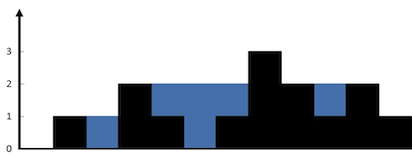
\includegraphics[width=.9\linewidth]{./pic/rainwatertrap.png}
\caption{Trapping Rain Water}
\end{figure}

The above elevation map is represented by array [0, 1, 0, 2, 1, 0, 1, 3, 2, 1, 2, 1]. In this case, 6 units of rain water (blue section) are being trapped. Thanks Marcos for contributing this image!

\textbf{Tags:} Array, Stack, Two Pointers

对于每个柱 子,找到其左右两边最 高的柱子, 该柱子能容纳的面积就是 min(max$_{\text{left}}$, max$_{\text{right}}$) - height。所以,

\begin{enumerate}
\item 从左往右扫描一遍,对于每个柱子,求取左边最大值;
\item 从右往左扫描一遍,对于每个柱子,求最大右值;
\item 再扫描一遍,把每个柱子的面积并累加。
\end{enumerate}
也可以,
\begin{enumerate}
\item 扫描一遍,找到最高的柱子,这个柱子将数组分为两半;
\item 处理左边一半;
\item 处理右边一半。
\end{enumerate}
\begin{enumerate}
\item 思路 1, 时间复杂度 O(n), 空间复杂度 O(n)
\label{sec-5-3-2-1}
\item 思路 2, 时间复杂度 O(n), 空间复杂度 O(1)
\label{sec-5-3-2-2}
\item 思路 3, 时间复杂度 O(n), 空间复杂度 O(n)
\label{sec-5-3-2-3}
\item 
\label{sec-5-3-2-4}
\end{enumerate}
\subsection{Largest Rectangle in Histogram}
\label{sec-5-3-3}
Given n non-negative integers representing the histogram's bar height where the width of each bar is 1, find the area of largest rectangle in the histogram.

\begin{figure}[htb]
\centering
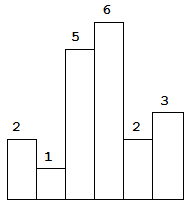
\includegraphics[width=.9\linewidth]{./pic/rectangle1.png}
\caption{Largest Rectangle in Histogram 1}
\end{figure}

Above is a histogram where width of each bar is 1, given height = [2, 1, 5, 6, 2, 3].

\begin{figure}[htb]
\centering
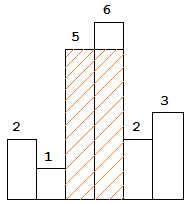
\includegraphics[width=.9\linewidth]{./pic/rectangle2.png}
\caption{Largest Rectangle in Histogram 2}
\end{figure}

The largest rectangle is shown in the shaded area, which has area = 10 unit.

For example,

Given height = [2, 1, 5, 6, 2, 3],

return 10.

简单的, 类似于 Container With Most Water(), 对每个柱子, 左右扩展, 直到碰到比自己矮的, 计算这个矩形的面积, 用一个变量记录最大的面积, 复杂度 O(n$^{\text{2}}$ ), 会超时。

如图所示, 从左到右处理直方, 当 i = 4 时, 小于当前栈顶(即直方 3),  对于直方 3, 无论后面还是前面的直方, 都不可能得到比目前栈顶元素更高的高度了, 处理掉直方 3(计算从直方 3到直方 4 之间的矩形的面积, 然后从栈里弹出); 对于直方 2 也是如此; 直到碰到比直方 4 更矮的直方 1。

这就意味着, 可以维护一个递增的栈, 每次比较栈顶与当前元素。如果当前元素小于栈顶元素, 则入栈, 否则合并现有栈, 直至栈顶元素小于当前元素。结尾时入栈元素 0, 重复合并一次。
\begin{enumerate}
\item O (n$^{\text{2}}$)
\label{sec-5-3-3-1}

最暴力的方法就是枚举所有区间的最大矩形值,然后选择最大的。可以通过分别枚举区间右边界和区间左边界,时间复杂度O(n$^{\text{2}}$)这样做大数据会超时。

枚举的过程中可以优化一下: 如果 height[i+1] > height[i], 那么区间 [k\ldots{}i] 内的最大矩形肯定不会超过区间 [k\ldots{}i+1] 内的最大矩形, 比如上例中的区间 [0\ldots{}3] 内的矩形要大于 [0\ldots{}2] 内的矩形, 因为 height[ 3 ] > height[ 2 ]。因此我们在枚举区间右边界时,只选择那些 height 上升区间的最大值处作为右边界(比如例子中的2 、6 、3)。优化后可以通过leetcode的大数据,虽然做了优化,但是时间复杂度还是O(n$^{\text{2}}$)。

\lstset{language=java,label= ,caption= ,numbers=none}
\begin{lstlisting}
public int largestRectangleArea(int[] height) {
    int n = height.length;
    int res = 0;
    int right = 0;
    int local = 0;
    int minVal = 0;
    while (right < n) {
        if (right + 1 < n && height[right + 1] >= height[right])
            right++;
        else { // found right border
            minVal = height[right];
            for (int left = right; left >= 0; left--) {
                minVal = Math.min(minVal, height[left]);
                local = minVal * (right - left + 1);
                res = Math.max(res, local);
            }
            right++;
            local = 0;
            minVal = 0;
        }
    }
    return res;
}
\end{lstlisting}

\item 栈: 时间复杂度 O(n), 空间复杂度 O(n)。
\label{sec-5-3-3-2}

主要思路:

我们知道,每个木板将对应多个包含自身的直方图面积,我们从中选取最大的一个面积。

以上题为例,height[ 1 ]对应的包含自身直方图面积集合为 \{1, 2, 3, 4, 5, 6 \} ,我们只需要知道最大的面积 6 即可,其它的面积就不用考虑。

我们就比较所有height[i] 对应最大直方图面积,把整体最大的直方图面积记为maxArea。

分析到这,我们很明显的可以知道时间复杂度为 O(n)。

现在关键问题就变为如何得到 height[i] 对应的最大直方图面积。

这里用一个栈s来保存之前的元素索引。

s为空时,直接让 i 栈: 以下取 i 从 0 到 n-1 。

\begin{itemize}
\item 当 height[i] < height[s.top()] 时,说明 height[s.top()] 对应的直方图面积不会再增加了,此时达到最大,可以出栈了;

\item 当 height[i] >= height[s.top()] 时,说明 height[s.top()] 对应的直方图面积还是有潜力增加的哈,此时,i 入栈,++i 。
\end{itemize}

当 i 达到 n 时,而栈不为空,说明还有部分height中元素对应的最大直方图面积没有求出来.

于是,当栈不为空时,求 height[s.top()] 对应最大直方图面积。

\lstset{language=java,label= ,caption= ,numbers=none}
\begin{lstlisting}
public int largestRectangleArea(int[] height) {
    Stack<Integer> s = new Stack<Integer>();
    int [] hnew = new int[height.length + 1];// 数组末尾插入 dummy 元素 0
    hnew = Arrays.copyOf(height, height.length + 1);
    int res = 0; 
    int tmp;     
    int left;
    for (int i = 0; i <= height.length; i++) {
        if (s.isEmpty() || hnew[i] > hnew[s.peek()])
            s.push(i); // 栈内保存的是数组 height 的下标索引
        else {
            tmp = s.pop();
            res = Math.max(res, hnew[tmp] * 
                           (s.isEmpty() ? i : i - s.peek() - 1));
            i--;
        }
    }
    return res;
}
\end{lstlisting}

这题应该还有很多很巧妙的解法,念天脑袋不太转,暂时留在这里吧,改天再回来修改\textasciitilde{}~

\url{http://www.cnblogs.com/felixfang/p/3676193.html}
\end{enumerate}

\section{others Covered}
\label{sec-5-4}
\begin{itemize}
\item Binary Tree Preorder Traversal
\ref{sec-4-1-1}
\item Binary Tree Inorder Traversal
\ref{sec-4-1-2}
\item Binary Tree Postorder Traversal
\ref{sec-4-1-3}
\item Binary Search Tree Iterator        
\ref{sec-4-4-9}
\item Binary Tree Zigzag Level Order Traversal
\ref{sec-4-1-6}
\item Maximal Rectangle
\ref{sec-14-3-3}
\item Min Stack
\ref{sec-19-1-2}
\end{itemize}
\chapter{Hash Table}
\label{sec-6}
\section{Easy}
\label{sec-6-1}
\subsection{Valid Sudoku}
\label{sec-6-1-1}
\subsection{Two Sum III}
\label{sec-6-1-2}
\section{Medium}
\label{sec-6-2}
\subsection{Two Sum}
\label{sec-6-2-1}
\subsection{4Sum}
\label{sec-6-2-2}
\subsection{Binary Tree Inorder Traversal}
\label{sec-6-2-3}
\subsection{Fraction to Recurring Decimal}
\label{sec-6-2-4}
\subsection{Single Number}
\label{sec-6-2-5}
\subsection{Anagrams}
\label{sec-6-2-6}
\subsection{Longest Substring Without Repeating Characters}
\label{sec-6-2-7}
\section{Hard}
\label{sec-6-3}
\subsection{Minimum Window Substring}
\label{sec-6-3-1}
\subsection{Copy List with Random Pointer}
\label{sec-6-3-2}
\subsection{Sudoku Solver}
\label{sec-6-3-3}
\subsection{Max Points on a Line}
\label{sec-6-3-4}
\subsection{Substring with Concatenation of All Words}
\label{sec-6-3-5}
\subsection{Longest Substring with At Most Two Distinct Characters}
\label{sec-6-3-6}
\section{other Covered}
\label{sec-6-4}
\begin{itemize}
\item Maximal Rectangle
\ref{sec-14-3-3}
\end{itemize}
\chapter{排序}
\label{sec-7}
\section{Easy}
\label{sec-7-1}
\subsection{Merge Sorted Array}
\label{sec-7-1-1}
Given two sorted integer arrays A and B, merge B into A as one sorted array.

Note:

You may assume that A has enough space (size that is greater or equal to m + n) to hold additional elements from B. The number of elements initialized in A and B are m and n respectively.

时间复杂度 O(m+n), 空间复杂度 O(1). 

\lstset{language=java,label= ,caption= ,numbers=none}
\begin{lstlisting}
public void merge(int a[], int m, int b[], int n) {
    int ia = m - 1;
    int ib = n - 1;
    int icur = m + n - 1;
    while (ia >= 0 && ib >= 0) 
        a[icur--] = a[ia] > b[ib] ? a[ia--] : b[ib--];
    while (ib >= 0) 
        a[icur--] = b[ib--];
}
\end{lstlisting}

\subsection{Merge Two Sorted List}
\label{sec-7-1-2}
Merge two sorted linked lists and return it as a new list. The new
list should be made by splicing together the nodes of the first two
lists.

时间复杂度 O(m+n), 空间复杂度 O(1).

\lstset{language=java,label= ,caption= ,numbers=none}
\begin{lstlisting}
public ListNode mergeTwoLists(ListNode l1, ListNode l2) {
    ListNode head = new ListNode(-1);     // dummy List ~!
    for (ListNode p = head; l1 != null || l2 != null; p = p.next) {
        int val1 = l1 == null ? Integer.MAX_VALUE : l1.val;
        int val2 = l2 == null ? Integer.MAX_VALUE : l2.val;
        if (val1 < val2) {
            p.next = l1;
            l1 = l1.next;
        } else {
            p.next = l2;
            l2 = l2.next;
        }
    }
    return head.next;
}
\end{lstlisting}

\section{Medium}
\label{sec-7-2}
\subsection{Sort Colors}
\label{sec-7-2-1}
Given an array with n objects colored red, white or blue, sort them so that objects of the same color are adjacent, with the colors in the order red, white and blue.

Here, we will use the integers 0, 1, and 2 to represent the color red, white, and blue respectively.

Note:

You are not suppose to use the library's sort function for this problem.

click to show follow up.

Follow up:

A rather straight forward solution is a two-pass algorithm using counting sort.

First, iterate the array counting number of 0's, 1's, and 2's, then overwrite array with total number of 0's, then 1's and followed by 2's.

Could you come up with an one-pass algorithm using only constant space?

\textbf{Tags:} Array, Two Pointers, Sort

由于 0, 1, 2 非常紧凑,首先想到计数排序 (counting sort),但需要扫描两遍,不符合题目要求。

由于只有三种颜色,可以设置两个 index,一个是 red 的 index,一个是 blue 的 index,两边往中
间走。时间复杂度 O(n),空间复杂度 O(1)。

第 3 种思路,利用快速排序里 partition 的思想,第一次将数组按 0 分割,第二次按 1 分割,排
序完毕,可以推广到 n 种颜色,每种颜色有重复元素的情况。

时间复杂度 O(n), 空间复杂度 O(1). 

\begin{enumerate}
\item Counting Sort: 时间复杂度 O(n), 空间复杂度 O(1)
\label{sec-7-2-1-1}

\lstset{language=java,label= ,caption= ,numbers=none}
\begin{lstlisting}
public void sortColors(int[] a) {
    int [] cnt = new int[3];  // 记录每个颜色出现的次数
    for (int i = 0; i < a.length; i++) 
        cnt[a[i]]++;
    for (int i = 0, index = 0; i < 3; i++) {
        for (int j = 0; j < cnt[i]; j++) {
            a[index++] = i;
        }
    }
}
\end{lstlisting}

\item 双指针: 时间复杂度 O(n), 空间复杂度 O(1)
\label{sec-7-2-1-2}
\lstset{language=java,label= ,caption= ,numbers=none}
\begin{lstlisting}
public void swap(int [] a, int i, int j) {
    int tmp = a[i];
    a[i] = a[j];
    a[j] = tmp;
}

public void sortColors(int[] a) {
    if (a == null || a.length < 2) return;
    int n = a.length;
    int i = 0;
    // 一个是 red 的 index,一个是 blue 的 index,两边往中间走
    int zEnd = -1;  // 0 end
    int tEnd = n;   // 2 end
    while (i < tEnd) {
        if (a[i] == 0 && i != ++zEnd) // first 0
            swap(a, zEnd, i);
        else if (a[i] == 2 && i != --tEnd)
            swap(a, i, tEnd);
        else i++;
    }
    return;
}
\end{lstlisting}

\item use partition():
\label{sec-7-2-1-3}
\item use partition():
\label{sec-7-2-1-4}
\end{enumerate}

\subsection{Sort List}
\label{sec-7-2-2}
Sort a linked list in O(n log n) time using constant space complexity.

\lstset{language=java,label= ,caption= ,numbers=none}
\begin{lstlisting}
public ListNode divideList(ListNode head) {
    ListNode fast = head;
    ListNode slow = head;
    ListNode prev = head;
    while (fast != null && fast.next != null) {
        prev = slow;
        slow = slow.next;
        fast = fast.next.next;
    }
    prev.next = null;
    return slow;
}

public ListNode mergeList(ListNode one, ListNode two) {
    if (one == null) return two;
    if (two == null) return one;
    ListNode dummy = new ListNode(Integer.MIN_VALUE);
    ListNode curr = dummy;
    while (one != null && two != null) {
        if (one.val < two.val) {
            curr.next = one;
            one = one.next;
        } else {
            curr.next = two;
            two = two.next;
        }
        curr.next.next = null;
        curr = curr.next;
    }
    if (one != null) curr.next = one;
    else curr.next = two;
    return dummy.next;
}

public ListNode sortList(ListNode head) {
    if (head == null || head.next == null) 
        return head;
    ListNode second = divideList(head);
    ListNode firstSorted = sortList(head);
    ListNode secondSorted = sortList(second);
    return mergeList(firstSorted, secondSorted);
}
\end{lstlisting}

\section{Hard}
\label{sec-7-3}
\subsection{Merge k sorted Lists}
\label{sec-7-3-1}
Merge k sorted linked lists and return it as one sorted list. Analyze and describe its complexity.

\textbf{Tags}: Divide and Conquer, Linked List, Heap

可以复用 Merge Two Sorted Lists(见 Merge Two Sorted List \ref{sec-7-1-2})的函数

时间复杂度 O(n1 + n2 + \ldots{}),空间复杂度 O(1). 

\lstset{language=java,label= ,caption= ,numbers=none}
\begin{lstlisting}
public ListNode mergeTwoLists(ListNode l1, ListNode l2) {
    ListNode head = new ListNode(-1);     // dummy List ~!
    for (ListNode p = head; l1 != null || l2 != null; p = p.next) {
        int val1 = l1 == null ? Integer.MAX_VALUE : l1.val;
        int val2 = l2 == null ? Integer.MAX_VALUE : l2.val;
        if (val1 < val2) {
            p.next = l1;
            l1 = l1.next;
        } else {
            p.next = l2;
            l2 = l2.next;
        }
    }
    return head.next;
}

public ListNode mergeKLists(List<ListNode> lists) {
    if (lists.size() == 0) return null;
    ListNode p = lists.get(0);  // Time Limit Exceeded
    for (int i = 1; i < lists.size(); i++) {
        p = mergeTwoLists(p, lists.get(i));
    }
    return p;
}

public ListNode mergeKLists(List<ListNode> lists) {
    if (lists.size() == 0) return null;
    if (lists.size() == 1) return lists.get(0);
    if (lists.size() == 2) return mergeTwoLists(lists.get(0), lists.get(1));
    return mergeTwoLists((mergeKLists(lists.subList(0, lists.size() / 2))),
                         (mergeKLists(lists.subList(lists.size() / 2, lists.size()))));
}
\end{lstlisting}

\subsection{Insertion Sort List}
\label{sec-7-3-2}
Sort a linked list using insertion sort.

这个,代码过于混乱,需要优化。。。

\lstset{language=java,label= ,caption= ,numbers=none}
\begin{lstlisting}
public ListNode insertionSortList(ListNode head) {
    if (head == null) return null;
    ListNode prev = head;
    ListNode curr = head.next;
    ListNode next = head;
    ListNode tnext = head;
    ListNode tmp = head;
    while (curr != null) {
        next = curr.next;
        if (curr.val < prev.val) {
            prev.next = next;
            curr.next = null;
            if (curr.val < head.val) {
                curr.next = head;
                head = curr;
            } else {
                tmp = head;
                while (tmp.next != prev && curr.val > tmp.next.val) {
                    tmp = tmp.next;
                }
                tnext = tmp.next;
                tmp.next = curr;
                curr.next = tnext;
            }
            curr = next;
        } else {
            prev = curr;
            curr = curr.next;
        }
    }
    return head;
}
\end{lstlisting}
\subsection{First Missing Positive}
\label{sec-7-3-3}
Given an unsorted integer array, find the first missing positive integer.

For example,

Given [1, 2, 0] return 3, 

and [3, 4, -1, 1] return 2.

Your algorithm should run in O(n) time and uses constant space.

本质上是桶排序 (bucket sort),每当 A[i]!= i+1 的时候,将 A[i] 与 A[A[i]-1] 交换,直到无法
交换为止,终止条件是 A[i]== A[A[i]-1]。

\lstset{language=java,label= ,caption= ,numbers=none}
\begin{lstlisting}
public void swap(int [] a, int i, int j) {        
    int tmp = a[i];
    a[i] = a[j];
    a[j] = tmp;
}

public void bucket_sort(int [] a) {
    for (int i = 0; i < a.length; i++) {
        while (a[i] != i + 1) {
            if (a[i] <= 0 || a[i] > a.length || a[i] == a[i] - 1)
                break;
            swap(a, i, a[i] - 1);
        }
    }
}

// need to clean code
// 时间复杂度 O(n), 空间复杂度 O(1)
public int firstMissingPositive(int[] a) {
    // Time Limit Exceeded
    bucket_sort(a);
    for (int i = 0; i < a.length; i++) 
        if (a[i] != (i + 1))
            return i + 1;
    return a.length + 1;
}

public int firstMissingPositive0(int[] a) {
    if (a == null || a.length == 0) return 1;
    if (a.length == 1) return a[0] == 1 ? 2 : 1;

    int n = a.length;
    boolean equl = false;
    int i;
    for ( i = 0; i < n; i++) {
        if (a[i] < 0) continue;
        if (a[i] == n) {
            equl = true;
            continue;
        }
        while ( (i == 0 || (i != 0 && a[i] != i))
                && a[i] < n && a[i] > 0 ) {
            swap(a, i, a[i]);
            if (a[i] == n) {
                equl = true;
                break;
            }
            if ((a[i] > n || a[i] < 0) || (a[i] >= 0 && a[i] == a[a[i]]))
                break; // to avoid infite loop
        }
    }
    for ( i = 1; i < n; i++) 
        if (a[i] != i) return i;
    if (equl || a[0] == n) return n + 1;
    else return n;
}
\end{lstlisting}

\section{other Covered}
\label{sec-7-4}
\subsection{Largest Number}
\label{sec-7-4-1}
\subsection{Maximum Gap}
\label{sec-7-4-2}
\begin{itemize}
\item Merge Intervals
\item Insert Interval
\end{itemize}
\chapter{查找}
\label{sec-8}
\section{Medium}
\label{sec-8-1}
\subsection{Search for a Range}
\label{sec-8-1-1}
Given a sorted array of integers, find the starting and ending position of a given target value.

Your algorithm's runtime complexity must be in the order of O(log n).

If the target is not found in the array, return [-1, -1].

For example,

Given [5, 7, 7, 8, 8, 10] and target value 8,

return [3, 4].

\textbf{Tags:} Array, Binary Search

已经排好了序,用二分查找。

时间复杂度 O(logn), 空间复杂度 O(1). 

分两步来做,找一次第一个,找一次最后一个,返回。
\lstset{language=java,label= ,caption= ,numbers=none}
\begin{lstlisting}
public int searchFirsst(int [] a, int target, int start, int end) {
    if (start == end) return (a[end] == target) ? start : -1;
    if (start == end - 1) {
        if (a[start] == target) return start;
        else if (a[end] == target) return end;
        else return -1;
    }

    while (start < end - 1) {
        int mid = start + (end - start) / 2;
        if (a[mid] >= target) 
            end = mid;
        else 
            start = mid + 1;
    }
    if (start == end) return (a[end] == target) ? start : -1;
    if (start == end - 1) {
        if (a[start] == target) return start;
        else if (a[end] == target) return end;
        else return -1;
    }
    return -1;
}

public int searchLast(int [] a, int target, int start, int end) {
    if (start == end) return (a[end] == target) ? end : -1;
    if (start == end - 1) {
        if (a[end] == target) return end;        
        else if (a[start] == target) return start;
        else return -1;
    }

    while (start < end - 1) {
        int mid = start + (end - start) / 2;
        if (a[mid] > target) 
            end = mid - 1;
        else 
            start = mid;
    }
    if (start == end) return (a[end] == target) ? end : -1;
    if (start == end - 1) {
        if (a[end] == target) return end;        
        else if (a[start] == target) return start;
        else return -1;
    }
    return -1;
}

public int[] searchRange(int[] A, int target) {
    int [] res = new int[2];
    if (A == null || A.length == 0 ||
        (A.length == 1 && A[0] != target)) {
        res[0] = -1;
        res[1] = -1;
        return res;   
    } else if (A.length == 1) {
        res[0] = 0;
        res[1] = 0;
        return res;   
    }
    res[0] = searchFirsst(A, target, 0, A.length-1);
    res[1] = searchLast(A, target, 0, A.length-1);
    return res;
}
\end{lstlisting}

\subsection{Search Insert Position}
\label{sec-8-1-2}
Given a sorted array and a target value, return the index if the target is found. If not, return the index where it would be if it were inserted in order.

You may assume no duplicates in the array.

Here are few examples.
\lstset{language=java,label= ,caption= ,numbers=none}
\begin{lstlisting}
[1, 3, 5, 6],  5 → 2
[1, 3, 5, 6],  2 → 1
[1, 3, 5, 6],  7 → 4
[1, 3, 5, 6],  0 → 0
\end{lstlisting}

直接的二分查找,查找第一个大于或等于target的位置。对于中间位置mid:

~ 如果 A[mid] >= target,那么答案至少应该为mid,或者为mid的左边
位置,则 end = mid

~ 否则 A[mid] < target,那么答案肯定在mid的右边,而且不可能为mid,则
bgn = mid +1

时间复杂度 O(logn), 空间复杂度 O(1). 
\lstset{language=java,label= ,caption= ,numbers=none}
\begin{lstlisting}
public int searchInsert(int[] a, int target) {
    int bgn = 0, end = a.length - 1;
    while (bgn <= end) {
        int mid = bgn + (end - bgn) / 2;
        if (a[mid] ==  target) return mid;
        if (mid > bgn && a[mid] > target && a[mid - 1] < target) return mid;
        if (a[mid] > target)
            end = mid - 1;
        else
            bgn = mid + 1;
    }
    return bgn;
}
\end{lstlisting}

\subsection{Search a 2D Matrix}
\label{sec-8-1-3}
Write an efficient algorithm that searches for a value in an m x n matrix. This matrix has the following properties:

Integers in each row are sorted from left to right.

The first integer of each row is greater than the last integer of the previous row.

For example,

Consider the following matrix:
\lstset{language=java,label= ,caption= ,numbers=none}
\begin{lstlisting}
[
  [1,   3,  5,  7],
  [10, 11, 16, 20],
  [23, 30, 34, 50]
]
\end{lstlisting}

Given target = 3, return true.

二分查找。

时间复杂度 O(logn), 空间复杂度 O(1). 

\lstset{language=java,label= ,caption= ,numbers=none}
\begin{lstlisting}
public boolean binarySearch(int [] a, int target, int bgn, int end) {
    while (bgn <= end) {
        int mid = bgn + (end - bgn) / 2;
        if (a[mid] == target) return true;
        if (a[mid] > target) end = mid - 1;
        else bgn = mid + 1;
    }
    return false;
}

public boolean searchMatrix(int[][] matrix, int target) {
    int m = matrix.length;
    int n = matrix[0].length;
    int [] a = new int[m * n];
    int cnt = 0;
    for (int i = 0; i < m; i++) 
        for (int j = 0; j < n; j++) 
            a[cnt++] = matrix[i][j];
    return binarySearch(a, target, 0, m * n - 1);
}
\end{lstlisting}

也可以把两个函数合并成一个,,省去中间合成桥梁数组的步骤,代码如下: 
\lstset{language=java,label= ,caption= ,numbers=none}
\begin{lstlisting}
public boolean searchMatrix(int[][] matrix, int target) {
    int m = matrix.length;
    int n = matrix[0].length;
    int bgn = 0;
    int end = m * n- 1;
    while (bgn <= end) {
        int mid = bgn + (end - bgn) / 2;
        int val = matrix[mid / n][mid % n];
        if (val == target) return true;
        if (val > target) end = mid - 1;
        else bgn = mid + 1;
    }
    return false;
}
\end{lstlisting}

\chapter{暴力枚举法}
\label{sec-9}
\section{Medium}
\label{sec-9-1}
\subsection{Subsets}
\label{sec-9-1-1}
Given a set of distinct integers, S, return all possible subsets.

Note:
\begin{itemize}
\item Elements in a subset must be in non-descending order.
\item The solution set must not contain duplicate subsets.
\end{itemize}
For example,

If S = [1,2,3], a solution is:
\lstset{language=java,label= ,caption= ,numbers=none}
\begin{lstlisting}
[
  [3],
  [1],
  [2],
  [1,2,3],
  [1,3],
  [2,3],
  [1,2],
  []
]
\end{lstlisting}

\textbf{Tags:} Array Backtracking, Bit Manipulation

\begin{enumerate}
\item 递归, 增量构造法: 增量构造法,深搜,时间复杂度 O(2$^{\text{n}}$), 空间复杂度 O(n)
\label{sec-9-1-1-1}

每个元素, 都有两种选择, 选或者不选。

\lstset{language=java,label= ,caption= ,numbers=none}
\begin{lstlisting}
public void helper(int [] s, List<Integer> path, int step, List<List<Integer>> res) {
    if (step == s.length) {
        res.add(new ArrayList<Integer>(path));
        return;   
    }
    helper(s, path, step + 1, res);  // 不选 S[step]
    path.add(s[step]);               // 选 S[step]
    helper(s, path, step + 1, res);
    path.remove(path.size() - 1);
}

public List<List<Integer>> subsets(int[] s) {
    Arrays.sort(s);           // 输出要求有序
    List<List<Integer>> res = new ArrayList<List<Integer>>();
    List<Integer> path = new ArrayList<Integer>();
    helper(s, path, 0, res);
    return res;
}
\end{lstlisting}
\item 递归, 位向量法: 时间复杂度 O(2$^{\text{n}}$), 空间复杂度 O(n).
\label{sec-9-1-1-2}

开一个位向量 bool selected[n],每个元素可以选或者不选。

位向量法, 深搜, 时间复杂度 O(2$^{\text{n}}$), 空间复杂度 O(n). 

\lstset{language=java,label= ,caption= ,numbers=none}
\begin{lstlisting}
public void helper(int [] s, boolean [] selected, int step, List<List<Integer>> res) {
    if (step == s.length) {
        List<Integer> path = new ArrayList<Integer>();
        for (int i = 0; i < s.length; i++) {
            if (selected[i]) path.add(s[i]);
        }
        res.add(path);
        return;   
    }
    selected[step] = false;
    helper(s, selected, step + 1, res);
    selected[step] = true;
    helper(s, selected, step + 1, res);
}

public List<List<Integer>> subsets(int[] s) {
    Arrays.sort(s); 
    List<List<Integer>> res = new ArrayList<List<Integer>>();
    boolean [] selected = new boolean[s.length];
    helper(s, selected, 0, res);
    return res;
}
\end{lstlisting}

\item 迭代, 增量构造法, 时间复杂度 O(2$^{\text{n}}$),空间复杂度 O(1)
\label{sec-9-1-1-3}

\lstset{language=java,label= ,caption= ,numbers=none}
\begin{lstlisting}
vector<vector<int> > subsets(vector<int> &S) {
    sort(S.begin(), S.end()); // 输出要求有序
    vector<vector<int> > result(1);
    for (auto elem : S) {
        result.reserve(result.size() * 2);
        auto half = result.begin() + result.size();
        copy(result.begin(), half, back_inserter(result));
        for_each(half, result.end(), [&elem](decltype(result[0]) &e){
                e.push_back(elem);
            });
    }
    return result;
}
\end{lstlisting}

需要改写成 Java 版。

\item 二进制法
\label{sec-9-1-1-4}

本方法的前提是:集合的元素不超过 int 位数。用一个 int 整数表示位向量, 第 i 位为 1, 则表示选择 S[i], 为 0 则不选择。例如 S=\{A, B, C, D\}, 则 0110=6 表示子集 \{B, C\}。

这种方法最巧妙。因为它不仅能生成子集, 还能方便的表示集合的并、交、差等集合运算。设两个集合的位向量分别为 B1 和 B2 , 则 B1 | B2 ,  B1 \& B2 ,  B1 B2 分别对应集合的并、交、对称差。

二进制法, 也可以看做是位向量法, 只不过更加优化。

二进制法, 时间复杂度 O(2$^{\text{n}}$), 空间复杂度 O(1)

\lstset{language=java,label= ,caption= ,numbers=none}
\begin{lstlisting}
public List<List<Integer>> subsets(int[] s) {
    Arrays.sort(s);   
    List<List<Integer>> res = new ArrayList<List<Integer>>();
    List<Integer> path = new ArrayList<Integer>();
    int n = s.length;
    for (int i = 0; i < (1 << n); i++) {
        for (int j = 0; j < n; j++) {
            // if ((i & (1 << j)) != 0) path.add(s[j]);
            if(((i >> j) & 1 ) != 0) path.add(s[j]);   
        }
        res.add(path);
        path = new ArrayList<Integer>();
    }
    return res;
}
\end{lstlisting}

总体看来,不管是用向量数组来保存选与不选,还是位操作,都是选与不选的控
制。通过有序控制来得到想要的结果。
\end{enumerate}

\subsection{Subsets II}
\label{sec-9-1-2}
Given a collection of integers that might contain duplicates, S, return all possible subsets.

Note:
\begin{itemize}
\item Elements in a subset must be in non-descending order.
\item The solution set must not contain duplicate subsets.
\end{itemize}
For example,

If S = [1,2,2], a solution is:
\lstset{language=java,label= ,caption= ,numbers=none}
\begin{lstlisting}
[
  [2],
  [1],
  [1,2,2],
  [2,2],
  [1,2],
  []
]
\end{lstlisting}

这题有重复元素,但本质上,跟上一题很类似,上一题中元素没有重复,相当于每个元素只能选 0 或 1 次,这里扩充到了每个元素可以选 0 到若干次而已。

\begin{enumerate}
\item 递归, 增量构造法: 增量构造法,深搜,时间复杂度 O(2$^{\text{n}}$), 空间复杂度 O(n)
\label{sec-9-1-2-1}


\lstset{language=java,label= ,caption= ,numbers=none}
\begin{lstlisting}
public void helper(int [] s, List<Integer> path, List<List<Integer>> res) {
    res.add(new ArrayList<Integer>(path));
    for (int i = 0; i < s.length; i++) {
        if (i != 0 && s[i] == s[i - 1]) continue;
        path.add(s[i]);
        helper(s, path, res);
        path.remove(path.size() - 1);
    }
}

// Memory Limit Exceeded
public List<List<Integer>> subsetsWithDup(int[] s) {
    Arrays.sort(s); 
    List<List<Integer>> res = new ArrayList<List<Integer>>();
    List<Integer> path = new ArrayList<Integer>();
    helper(s, path, res);
    return res;
}
\end{lstlisting}

\item 增量构造法,版本 2,时间复杂度 O(2$^{\text{n}}$),空间复杂度 O(n)
\label{sec-9-1-2-2}
\item 位向量法, 时间复杂度 O(2$^{\text{n}}$), 空间复杂度 O(n)
\label{sec-9-1-2-3}

这个相对复杂,改天再写
\item 迭代, 增量构造法, 时间复杂度 O(2$^{\text{n}}$),空间复杂度 O(1)
\label{sec-9-1-2-4}


\item 二进制法
\label{sec-9-1-2-5}

\lstset{language=java,label= ,caption= ,numbers=none}
\begin{lstlisting}
public List<List<Integer>> subsetsWithDup(int[] s) {
    Arrays.sort(s);   
    HashSet<List<Integer>> res = new HashSet<List<Integer>>();
    List<Integer> path = new ArrayList<Integer>();
    int n = s.length;
    for (int i = 0; i < (1 << n); i++) {
        for (int j = 0; j < n; j++) {
            if ((i & (1 << j)) != 0) path.add(s[j]);
            //if(((i >> j) & 1 ) != 0) path.add(s[j]);   
        }
        res.add(path);
        path = new ArrayList<Integer>();
    }
    List<List<Integer>> result = new ArrayList<List<Integer>>();
    result.addAll(res);
    return result;
}
\end{lstlisting}

与上一题类似,只是多一步控制对重复的处理,或不再执行重复的,或执行后去
重处理。
\end{enumerate}

\subsection{Permutation}
\label{sec-9-1-3}
Given a collection of numbers, return all possible permutations.

For example,
\lstset{language=java,label= ,caption= ,numbers=none}
\begin{lstlisting}
[1,2,3] have the following permutations:
[1,2,3], [1,3,2], [2,1,3], [2,3,1], [3,1,2], and [3,2,1].
\end{lstlisting}

偷懒的做法,可以直接使用 c++ std::next$_{\text{permutation}}$()。如果是在 OJ 网站上,可以用这个API 偷个懒;如果是在面试中,面试官肯定会让你重新实现。

时间复杂度 O(n!),空间复杂度 O(1)

\begin{enumerate}
\item 重新实现 next$_{\text{permutation}}$(): 时间复杂度 O(n!), 空间复杂度 O(1)
\label{sec-9-1-3-1}
\item 递归: 时间复杂度 O(n!), 空间复杂度 O(n)
\label{sec-9-1-3-2}

本题是求路径本身,求所有解,函数参数需要标记当前走到了哪步,还需要中间结果的引用,最终结果的引用。

扩展节点,每次从左到右,选一个没有出现过的元素。

本题不需要判重,因为状态装换图是一颗有层次的树。收敛条件是当前走到了最
后一个元素。

\lstset{language=java,label= ,caption= ,numbers=none}
\begin{lstlisting}
public void helper(int [] num, boolean [] used, List<Integer> one,
                   List<List<Integer>> res) {
    if (one.size() == num.length) {
        res.add(new ArrayList<Integer>(one));
        return;
    }
    for (int i = 0; i < num.length; i++) {
        if (!used[i]) {
            used[i] = true;
            one.add(num[i]);
            helper(num, used, one, res);
            one.remove(one.size() - 1);
            used[i] = false;
        }
    }
    return;
}

public List<List<Integer>> permute(int[] num) {
    List<List<Integer>> res = new ArrayList<List<Integer>>();
    if (num == null || num.length == 0) return res;
    boolean [] used = new boolean[num.length];
    helper(num, used, new ArrayList<Integer>(), res);
    return res;
}
\end{lstlisting}
\end{enumerate}

\subsection{Combinationas}
\label{sec-9-1-4}
Given two integers n and k, return all possible combinations of k numbers out of 1 \ldots{} n.

For example,

If n = 4 and k = 2, a solution is:
\lstset{language=java,label= ,caption= ,numbers=none}
\begin{lstlisting}
[
  [2,4],
  [3,4],
  [2,3],
  [1,2],
  [1,3],
  [1,4],
]
\end{lstlisting}
\begin{enumerate}
\item 递归: 深搜, 时间复杂度 O(n!), 空间复杂度 O(n)
\label{sec-9-1-4-1}

时间复杂度 O(n!), 空间复杂度 O(n). 
\lstset{language=java,label= ,caption= ,numbers=none}
\begin{lstlisting}
// bgn, 开始的数, cur, 已经选择的数目
public void dfs(List<List<Integer>> res, List<Integer> path, int n, int k, int bgn, int cur) {
    if (cur == k) {
        res.add(new ArrayList<Integer>(path));
    }
    for (int i = bgn; i <= n; i ++) {
        path.add(i);
        dfs(res, new ArrayList<Integer>(path), n, k, i + 1, cur + 1);
        path.remove(path.size() - 1);
    }
}

public List<List<Integer>> combine(int n, int k) {
    List<List<Integer>> res = new ArrayList<List<Integer>>();
    List<Integer> path = new ArrayList<Integer>();
    dfs(res, path, n, k, 1, 0); 
    return res;
}
\end{lstlisting}
\item 迭代: 时间复杂度 O((n-k)!), 空间复杂度 O(n)
\label{sec-9-1-4-2}

时间复杂度 O((n-k)!), 空间复杂度 O(n). 

some other day\textasciitilde{}~!!@
\end{enumerate}

\subsection{Letter Combinationas of Phone Number}
\label{sec-9-1-5}
Given a digit string, return all possible letter combinations that the number could represent.

A mapping of digit to letters (just like on the telephone buttons) is given below.

\begin{figure}[htb]
\centering
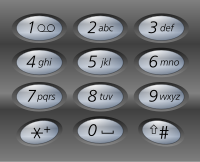
\includegraphics[width=.9\linewidth]{./pic/phoneNumber.png}
\caption{Letter Combinationas of Phone Number}
\end{figure}
\lstset{language=java,label= ,caption= ,numbers=none}
\begin{lstlisting}
Input:Digit string "23"
Output: ["ad", "ae", "af", "bd", "be", "bf", "cd", "ce", "cf"].
\end{lstlisting}
Note:

Although the above answer is in lexicographical order, your answer
could be in any order you want.

\begin{enumerate}
\item 递归: 深搜, 时间复杂度 O(3$^{\text{n}}$), 空间复杂度 O(n)
\label{sec-9-1-5-1}

\lstset{language=java,label= ,caption= ,numbers=none}
\begin{lstlisting}
public char [] getArr(char x) {
    char [] two = {'a', 'b', 'c'};
    char [] thr = {'d', 'e', 'f'};
    char [] fou = {'g', 'h', 'i'};
    char [] fiv = {'j', 'k', 'l'};
    char [] six = {'m', 'n', 'o'};
    char [] sev = {'p', 'q', 'r', 's'};
    char [] eig = {'t', 'u', 'v'};
    char [] nin = {'w', 'x', 'y', 'z'};
    switch (x) {
    case '2': return two;
    case '3': return thr;
    case '4': return fou;
    case '5': return fiv;
    case '6': return six;
    case '7': return sev;
    case '8': return eig;
    case '9': return nin;
    }
    return null;
}

public void recursion(String digits, List<String> result) {
    char [] base = getArr(digits.charAt(digits.length()-1));
    int n = result.size();
    //for(String x : result) // ConcurrentModificationException, result is changing
    for (int j = 0; j < n; j++) {
        for (int i = 0; i < base.length; i++)
            result.add(new StringBuffer(base[i]+ result.get(j)).toString());
    }
    for (int i = n-1; i >= 0; i--)
        result.remove(i);
    if (digits.length() > 1)
        recursion(digits.substring(0, digits.length()-1), result);
}

public List<String> letterCombinations(String digits) {
    List<String> result = new ArrayList<String>();
    if (digits.equals("")) {
        result.add("");
        return result;
    }
    char [] base = getArr(digits.charAt(digits.length()-1));
    for (int i = 0; i < base.length; i++) 
        result.add("" + base[i]);
    if (digits.length() > 1)
        recursion(digits.substring(0, digits.length()-1), result);
    return result;
}
\end{lstlisting}

\item 迭代: 时间复杂度 O(3$^{\text{n}}$), 空间复杂度 O(1)
\label{sec-9-1-5-2}
\end{enumerate}

\section{Hard}
\label{sec-9-2}
\subsection{Permutation II}
\label{sec-9-2-1}
Given a collection of numbers that might contain duplicates, return all possible unique permutations.

For example,
\lstset{language=java,label= ,caption= ,numbers=none}
\begin{lstlisting}
[1,1,2] have the following unique permutations:
[1,1,2], [1,2,1], and [2,1,1].
\end{lstlisting}

\begin{enumerate}
\item next$_{\text{permutation}}$()
\label{sec-9-2-1-1}

直接使用 std::next$_{\text{permutation}}$(),代码与上一题相同。
\item 重新实现 next$_{\text{permutation}}$()
\label{sec-9-2-1-2}

重新实现 std::next$_{\text{permutation}}$(),代码与上一题相同。
\item 递归:
\label{sec-9-2-1-3}

递归函数 permute() 的参数 p,是中间结果,它的长度又能标记当前走到了哪一步,用于判断收敛条件。

扩展节点,每次从小到大,选一个没有被用光的元素,直到所有元素被用光。

本题不需要判重,因为状态装换图是一颗有层次的树。

\lstset{language=java,label= ,caption= ,numbers=none}
\begin{lstlisting}
public void helper(int [] num, boolean [] used, List<Integer> one,
                   List<List<Integer>> res, int cnt) {
    if (one.size() == num.length) {
        res.add(new ArrayList<Integer>(one));
        return;
    }
    for (int i = 0; i < num.length; i++) {
        // !used[i - 1] marks the completion of first 0 done, so ignore second 0
        if (i > 0 && !used[i - 1] && num[i] == num[i - 1]) continue;
        if (!used[i]) {
            used[i] = true;
            one.add(num[i]);
            helper(num, used, one, res, ++cnt);
            one.remove(one.size() - 1);
            used[i] = false;
        }
    }
    return;
}

public List<List<Integer>> permuteUnique(int[] num) {
    List<List<Integer>> res = new ArrayList<List<Integer>>();
    if (num == null || num.length == 0) return res;
    boolean [] used = new boolean[num.length];
    Arrays.sort(num);
    helper(num, used, new ArrayList<Integer>(), res, 1);
    return res;
}
\end{lstlisting}

应该还有其它更好的控制原理,只是今天不在状态,不用多想。。。
\end{enumerate}

\chapter{广度优先搜索 Breadth First Search}
\label{sec-10}
当题目看不出任何规律, 既不能用分治, 贪心, 也不能用动规时, 这时候万能方法——搜索, 就派上用场了。搜索分为广搜和深搜, 广搜里面又有普通广搜, 双向广搜, A* 搜索等。深搜里面又有普通深搜, 回溯法等。

广搜和深搜非常类似(除了在扩展节点这部分不一样), 二者有相同的框架, 如何表示状态?如何扩展状态?如何判重?尤其是判重, 解决了这个问题, 基本上整个问题就解决了。
\section{Medium}
\label{sec-10-1}
\subsection{Surrounded Regions}
\label{sec-10-1-1}
Given a 2D board containing 'X' and 'O', capture all regions surrounded by 'X'.

A region is captured by flipping all 'O's into 'X's in that surrounded region.

For example,
\lstset{language=java,label= ,caption= ,numbers=none}
\begin{lstlisting}
X X X X
X O O X
X X O X
X O X X
\end{lstlisting}

After running your function, the board should be:
\lstset{language=java,label= ,caption= ,numbers=none}
\begin{lstlisting}
X X X X
X X X X
X X X X
X O X X
\end{lstlisting}

\textbf{Tags:} Breadth-first Search

广搜。从上下左右四个边界往里走,凡是能碰到的'O',都是跟边界接壤的,应该删
除。

这叫广搜啊? 我还以为延着0深搜呢。。。

四面的最外层搜索,有O通路的就为不被包围的区域,其他都可以置为X;没把握
这个特点,难度为五星级的。思路还是很新颖的。

注意栈溢出总题。

\lstset{language=java,label= ,caption= ,numbers=none}
\begin{lstlisting}
public void solve(char[][] board) {
    if (board.length == 0) return;
    int row = board.length;
    int col = board[0].length;
    for (int i = 0; i < row; i++) {
        for (int j = 0; j < col; j++) {
            if ((i == 0 || j == 0 || i == row-1 || j == col-1) && board[i][j] == 'O') {
                Stack<Integer> stk = new Stack<Integer>();
                stk.push(i * col + j);         // cannot *row, produce error, the larger 
                while (!stk.isEmpty()) {
                    int tmp = stk.pop();
                    int x = tmp / col;
                    int y = tmp % col;
                    if (x < 0 || y < 0 || x >= row || y >= col ||
                        !(board[x][y] == 'O'))
                        continue;
                    board[x][y] = '#';
                    stk.push((x-1) * col + y);
                    stk.push((x+1) * col + y);
                    stk.push(x * col + (y - 1));
                    stk.push(x * col + (y + 1));
                }
            }
        }
    }

    for (int i = 0; i < row; i++) {
        for (int j = 0; j < col; j++) {
            if (board[i][j] == 'O')
                board[i][j] = 'X';
            if (board[i][j] == '#')
                board[i][j] = 'O';
        }
    }
}
\end{lstlisting}

\subsection{Word Ladder}
\label{sec-10-1-2}
Given two words (start and end), and a dictionary, find the length of shortest transformation sequence from start to end, such that:
\begin{itemize}
\item Only one letter can be changed at a time
\item Each intermediate word must exist in the dictionary
\end{itemize}
For example,

Given:
\lstset{language=java,label= ,caption= ,numbers=none}
\begin{lstlisting}
start = "hit"
end = "cog"
dict = ["hot","dot","dog","lot","log"]
As one shortest transformation is "hit" -> "hot" -> "dot" -> "dog" -> "cog",
return its length 5.
\end{lstlisting}
Note:
\begin{itemize}
\item Return 0 if there is no such transformation sequence.
\item All words have the same length.
\item All words contain only lowercase alphabetic characters.
\end{itemize}

时间复杂度 O(n), 空间复杂度 O(n).

\begin{figure}[htb]
\centering
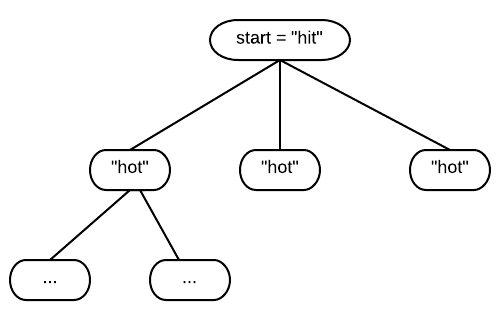
\includegraphics[width=.9\linewidth]{./pic/wordladder.png}
\caption{Word Ladder}
\end{figure}

分析:这种题,肯定是每次改变单词的一个字母,然后逐渐搜索,很多人一开始就想到用dfs,其实像这种求最短路径、树最小深度问题bfs最适合,可以参考我的这篇博客bfs(层序遍历)求二叉树的最小深度。本题bfs要注意的问题:

和当前单词相邻的单词是:对当前单词改变一个字母且在字典中存在的单词, 找到一个单词的相邻单词,加入bfs队列后,要从字典中删除,因为不删除的话会造成类似于hog->hot->hog的死循环。而删除对求最短路径没有影响,因为我们第一次找到该单词肯定是最短路径,即使后面其他单词也可能转化得到它,路径肯定不会比当前的路径短(如果要输出所有最短路径,则不能立即从字典中删除,具体见下一题)

bfs队列中用NULL来标识层与层的间隔,每次碰到层的结尾,遍历深度+1

我们利用和求二叉树最小深度层序遍历的方法来进行bfs,代码如下: 

\lstset{language=java,label= ,caption= ,numbers=none}
\begin{lstlisting}
public int ladderLength(String start, String end, Set<String> dict) {
    if (start.length() != end.length()) return 0;
    if (start.compareTo("") == 0) return 1;
    List<String> newStart = new ArrayList<String>();
    List<String> nextStart = new ArrayList<String>();
    newStart.add(start);
    int distance = 1;
    for (int index = 0; index < newStart.size(); index++) {
        String curr = newStart.get(index);
        for (int i = 0; i < curr.length(); i++) {
            for (char j = 'a'; j <= 'z'; j++) {
                if (curr.charAt(i) == j) continue;
                String tmp = curr.substring(0, i) + j + curr.substring(i + 1);
                if (tmp.equals(end)) return distance + 1;
                if (dict.contains(tmp)) {
                    nextStart.add(tmp);
                    dict.remove(tmp);
                }
            }
        }
        if (index == newStart.size() - 1) {
            newStart.addAll(new ArrayList<String>(nextStart));
            nextStart = new ArrayList<String>();
            distance++;
        }
    }
    return 0;
}
\end{lstlisting}

应该还有更多更好的方法,改天再深入去写。

\section{Hard}
\label{sec-10-2}
\subsection{Word Ladder II}
\label{sec-10-2-1}
Given two words (start and end), and a dictionary, find all shortest transformation sequence(s) from start to end, such that:
\begin{enumerate}
\item Only one letter can be changed at a time
\item Each intermediate word must exist in the dictionary
\end{enumerate}
For example,

Given:

start = "hit", end = "cog"

dict = ["hot","dot","dog","lot","log"]

Return
\lstset{language=java,label= ,caption= ,numbers=none}
\begin{lstlisting}
[
  ["hit","hot","dot","dog","cog"],
  ["hit","hot","lot","log","cog"]
]
\end{lstlisting}

Note:
\begin{itemize}
\item All words have the same length.
\item All words contain only lowercase alphabetic characters.
\end{itemize}

跟 Word Ladder 比,这题是求路径本身,不是路径长度,也是 BFS,略微麻烦点。

这题跟普通的广搜有很大的不同,就是要输出所有路径,因此在记录前驱和判重地方与普通广搜不同。

时间复杂度 O(n), 空间复杂度 O(n)。

这道题是LeetCode中AC率最低的题目,确实是比较难。一方面是因为对时间有比较严格的要求(容易超时),另一方面是它有很多细节需要实现。思路上和Word Ladder是比较类似的,但是因为是要求出所有路径,仅仅保存路径长度是不够的,而且这里还有更多的问题,那就是为了得到所有路径,不是每个结点访问一次就可以标记为visited了,因为有些访问过的结点也会是别的路径上的结点,所以访问的集合要进行回溯(也就是标记回未访问)。所以时间上不再是一次广度优先搜索的复杂度了,取决于结果路径的数量。同样空间上也是相当高的复杂度,因为我们要保存过程中满足的中间路径到某个数据结构中,以便最后可以获取路径,这里我们维护一个HashMap,把一个结点前驱结点都进行保存。

在LeetCode中用Java实现上述算法非常容易超时。为了提高算法效率,需要注意一下两点:

1)在替换String的某一位的字符时,先转换成char数组再操作;

2)如果按照正常的方法从start找end,然后根据这个来构造路径,代价会比较
高,因为保存前驱结点容易,而保存后驱结点则比较困难。所以我们在广度优先
搜索时反过来先从end找start,最后再根据生成的前驱结点映射从start往end构
造路径,这样算法效率会有明显提高。

\lstset{language=java,label= ,caption= ,numbers=none}
\begin{lstlisting}
/* Graph of example:
 *                |--- dot --- dog ---|
 * hit --- hot -- |     |       |     |--- cog
 *                |--- lot --- log ---|
 */
// set: visited   // current level used already
// set: unvisited // leftover for choosing for next level to avoid repeat, dict + end
// List<List<String>> res; // result paths
// List<String, Queue<String>> adjMap; // adjacent directed graph, 
// List<string, List<String>> works 2 ~! clone graph
\end{lstlisting}

\lstset{language=java,label= ,caption= ,numbers=none}
\begin{lstlisting}
private List<String> getNextLadder(String currLadder, Set<String> unVisited) {
    ArrayList<String> nextLadders = new ArrayList<String>();
    StringBuffer replace = new StringBuffer(currLadder); // mutate from here
    for(int i = 0; i < currLadder.length(); i++){
        char old = replace.charAt(i);
        for(char ch = 'a'; ch <= 'z'; ch++){
            if (currLadder.charAt(i) != ch) 
                replace.setCharAt(i, ch);
            else continue;
            String replaced = replace.toString();
            if (unVisited.contains(replaced)) 
                nextLadders.add(replaced);
        }
        replace.setCharAt(i, old); 
    }
    return nextLadders;
}

private void getLadders(String start, String end, LinkedList<String> path,
                        List<List<String>> res,
                        HashMap<String, Queue<String>> adjMap) {
    if (end.equals(start))      // end condition, len ?
        res.add(new ArrayList<String> (path));   
    else {                      // else if (len > 0) {            
        Queue<String> adjs = adjMap.get(end);
        for (String lad : adjs) {
            path.addFirst(lad); // path.add(0, lad); // equivallent
            getLadders(start, lad, path, res, adjMap);
            path.removeFirst(); // path.remove(0);   // remove ele at idx 0
        }
    }
}

public List<List<String>> findLadders(String start, String end, HashSet<String> dict) {
    HashMap<String, Queue<String>> adjMap = new HashMap<String, Queue<String>>(); 
    int currLen = 0;
    boolean found = false;
    List<List<String>> res = new ArrayList<List<String>>(); // results
    Queue<String> queue = new LinkedList<String>();         // queue for BFS
    Set<String> unv = new HashSet<String>(dict);            // unvstd words, delete f here
    Set<String> vst = new HashSet<String>();                // check vstd during same level
    unv.add(end);       // dict may not contain end, so we add it~!@
    queue.offer(start); // search & build from start
    int currLev = 1;
    int nextLev = 0;
    for(String word : unv)    // all strings in dict + start
        adjMap.put(word, new LinkedList<String>());  // just like clone graph
    unv.remove(start);
    while (!queue.isEmpty()) {
        String currLadder = queue.poll();  // curr word, mutate, check dicts, add or not
        for(String nextLadder : getNextLadder(currLadder, unv)){ 
            if (vst.add(nextLadder)) {  // add to vst set, return true, succeed, 
                nextLev++;              // vst set didn't contain it before
                queue.offer(nextLadder);
            }
            adjMap.get(nextLadder).offer(currLadder); 
            if(nextLadder.equals(end) && !found) { // control if start-->end, No here
                found = true;
                currLen += 2;
            }
        } 
        if(--currLev == 0){
            if(found) break;
            unv.removeAll(vst);  // remove all used string from cur level 
            currLev = nextLev;   // to avoid next level repeat & infinite loop
            nextLev = 0;
            currLen++;
        }
    }
    if (found) {
        LinkedList<String> path = new LinkedList<String>();
        path.addFirst(end);     // add at beginning of list
        getLadders(start, end, path, res, adjMap);
    }
    return res;
}
\end{lstlisting}

此题改天再回来优化。。。。

\section{other Covered}
\label{sec-10-3}
\begin{itemize}
\item Binary Tree Level Order Traversal
\ref{sec-4-1-4}
\item Binary Tree Level Order Traversal II
\ref{sec-4-1-5}
\item Clone Graph        
\ref{sec-18-1-1}
\item Binary Tree Zigzag Level Order Traversal
\ref{sec-4-1-6}
\item Minimum Depth of Binary Tree
\ref{sec-4-4-1}
\end{itemize}
\section{小结}
\label{sec-10-4}
\subsection{适用场景}
\label{sec-10-4-1}
\textbf{输入数据:} 没什么特征,不像深搜,需要有“递归”的性质。如果是树或者图,概率更大。

\textbf{状态转换图:} 树或者图。

\textbf{求解目标:} 求最短。
\subsection{思考的步骤}
\label{sec-10-4-2}
\begin{enumerate}
\item 求路径长度,还是路径本身(或动作序列)?
\label{sec-10-4-2-1}

(a) 如果是求路径长度,则状态里面要存路径长度

(b) 如果是求路径本身或动作序列

~ i. 要用一棵树存储宽搜过程中的路径

~ ii. 是否可以预估状态个数的上限?能够预估状态总数,则开一个大数组,用树的双亲
表示法;如果不能预估状态总数,则要使用一棵通用的树。这一步也是第 4 步的必
要不充分条件。
\item 如何表示状态?即一个状态需要存储哪些些必要的数据,才能够完整提供如何扩展到下一步状态的所有信息。一般记录当前位置或整体局面。
\label{sec-10-4-2-2}
\item 如何扩展状态?这一步跟第 2 步相关。状态里记录的数据不同,扩展方法就不同。对于固定不变的数据结构(一般题目直接给出,作为输入数据),如二叉树,图等,扩展方法很简单,直接往下一层走,对于隐式图,要先在第 1 步里想清楚状态所带的数据,想清楚了这点,那如何扩展就很简单了。
\label{sec-10-4-2-3}
\item 关于判重,状态是否存在完美哈希方案?即将状态一一映射到整数,互相之间不会冲突。
\label{sec-10-4-2-4}

(a) 如果不存在,则需要使用通用的哈希表(自己实现或用标准库,例如unordered\textunderscore{}set)
来判重;自己实现哈希表的话,如果能够预估状态个数的上限,则可以开两个数组,
head 和 next,表示哈希表,参考第 §??节方案 2。

(b) 如果存在,则可以开一个大布尔数组,作为哈希表来判重,且此时可以精确计算出状态
总数,而不仅仅是预估上限。
\item 目标状态是否已知?如果题目已经给出了目标状态,可以带来很大便利,这时候可以从起始状态出发,正向广搜;也可以从目标状态出发,逆向广搜;也可以同时出发,双向广搜。
\label{sec-10-4-2-5}
\end{enumerate}

\chapter{深度优先搜索 Depth First Search}
\label{sec-11}
\section{Medium}
\label{sec-11-1}
\subsection{Palindrome Partitioning}
\label{sec-11-1-1}
Given a string s, partition s such that every substring of the partition is a palindrome.

Return all possible palindrome partitioning of s.

For example, 
\lstset{language=java,label= ,caption= ,numbers=none}
\begin{lstlisting}
given s = "aab",
Return
  [
    ["aa","b"],
    ["a","a","b"]
  ]
\end{lstlisting}

在每一步都可以判断中间结果是否为合法结果,用回溯法。

一个长度为 n 的字符串,有 n+1 个地方可以砍断,每个地方可断可不断,前后两
个隔板默认已经使用,因此复杂度为 O(2$^{\text{n−1}}$).

\begin{enumerate}
\item 深搜: 时间复杂度 O(2$^{\text{n}}$), 空间复杂度 O(n)
\label{sec-11-1-1-1}
\lstset{language=java,label= ,caption= ,numbers=none}
\begin{lstlisting}
public void dfs(String s, List<String> path, List<List<String>> res) {
    if (s.length() == 0) {
        res.add(new ArrayList<String>(path));
        return;
    }
    for (int i = 0; i < s.length(); i++) {
        int bgn = 0;
        int end = i;
        while (bgn < end) {
            if (s.charAt(bgn) == s.charAt(end)) {
                bgn ++;
                end --;
            } else break;
        }
        if (bgn >= end) {
            path.add(s.substring(0, i + 1));
            dfs(s.substring(i + 1), path, res);
            path.remove(path.size() - 1);
        } 
    }
    return;
}

public List<List<String>> partition(String s) {
    List<List<String>> res = new ArrayList<List<String>>();
    List<String> path = new ArrayList<String>();
    dfs(s, path, res);
    return res;
}
\end{lstlisting}

\item 深搜 2: 时间复杂度 O(2$^{\text{n}}$), 空间复杂度 O(n)
\label{sec-11-1-1-2}

另一种写法,更加简洁。这种写法也在 Combination Sum, Combination Sum II 中出现过。

\item 动态规划:时间复杂度 O(n$^{\text{2}}$),空间复杂度 O(1)
\label{sec-11-1-1-3}

需要先消化一下别人的解法。。。。
\end{enumerate}

\subsection{Restore IP Addresses}
\label{sec-11-1-2}
Given a string containing only digits, restore it by returning all possible valid IP address combinations.

For example:
\lstset{language=java,label= ,caption= ,numbers=none}
\begin{lstlisting}
Given "25525511135",
return ["255.255.11.135", "255.255.111.35"]. (Order does not matter)
\end{lstlisting}

必须要走到底部才能判断解是否合法, 深搜。

需要优化自己的代码 ,写得太丑。。。

\subsection{Generate Parentheses}
\label{sec-11-1-3}
Given n pairs of parentheses, write a function to generate all combinations of well-formed parentheses.

For example, given n = 3, a solution set is:
\lstset{language=java,label= ,caption= ,numbers=none}
\begin{lstlisting}
"((()))", "(()())", "(())()", "()(())", "()()()"
\end{lstlisting}

小括号串是一个递归结构,跟单链表、二叉树等递归结构一样,首先想到用递归。

一步步构造字符串。当左括号出现次数 < n 时,就可以放置新的左括号。当右括号出现次数小
于左括号出现次数时,就可以放置新的右括号。

\begin{enumerate}
\item 时间复杂度 O(TODO),空间复杂度 O(n)
\label{sec-11-1-3-1}
\lstset{language=java,label= ,caption= ,numbers=none}
\begin{lstlisting}
public void generate(List<String> res, int n, StringBuffer one, int left, int right) {
    StringBuffer tmp = new StringBuffer(one);
    if (left == n) {
        for (int i = 0; i < n - right; i++)
            tmp.append(")");
        res.add(tmp.toString());
        return;
    }
    generate(res, n, new StringBuffer(one).append("("), left + 1, right);
    if (left > right)
        generate(res, n, new StringBuffer(one).append(")"), left, right + 1);
}

public List<String> generateParenthesis(int n) {
    List<String> res = new ArrayList<String>();
    if (n > 0)
        generate(res, n, new StringBuffer(), 0, 0);
    return res;
}
\end{lstlisting}

反过来写。
\lstset{language=java,label= ,caption= ,numbers=none}
\begin{lstlisting}
public void generate(List<String> res, int n, StringBuffer tmp, int left, int right) {
    if (left < 0 || right < left) return;
    if (left == 0 && right == 0) { 
        res.add(tmp.toString());
        return;
    } else {
        if (left > 0) 
            generate(res, n, new StringBuffer(tmp).append("("), left - 1, right);
        if (right > left) 
            generate(res, n, new StringBuffer(tmp).append(")"), left, right - 1);
    }
}

public List<String> generateParenthesis(int n) {
    List<String> res = new ArrayList<String>();
    if (n > 0) 
        generate(res, n, new StringBuffer(), n, n);
    return res;
}
\end{lstlisting}
不太确定这是真正正确的操作StringBuffer的途径还。

\item 另一种写法:
\label{sec-11-1-3-2}
\end{enumerate}
\subsection{Combination Sum}
\label{sec-11-1-4}
Given a set of candidate numbers (C) and a target number (T), find all unique combinations in C where the candidate numbers added to T.

The same repeated number may be chosen from C unlimited number of times.

Note:
\begin{itemize}
\item All numbers (including target) will be positive integers.
\item Elements in a combination (a1, a2, … , ak) must be in non-descending order. (ie, a1 ≤ a2 ≤ … ≤ ak).
\item The solution set must not contain duplicate combinations.
\end{itemize}

For example, given candidate set 2,3,6,7 and target 7, 

A solution set is: 
\lstset{language=java,label= ,caption= ,numbers=none}
\begin{lstlisting}
[7] 
[2, 2, 3]
\end{lstlisting}
\subsection{Combination Sum II}
\label{sec-11-1-5}
Given a collection of candidate numbers (C) and a target number (T), find all unique combinations in C where the candidate numbers added to T.

Each number in C may only be used once in the combination.

Note:
\begin{itemize}
\item All numbers (including target) will be positive integers.
\item Elements in a combination (a1, a2, … , ak) must be in non-descending order. (ie, a1 ≤ a2 ≤ … ≤ ak).
\item The solution set must not contain duplicate combinations.
\end{itemize}
For example, given candidate set 10,1,2,7,6,1,5 and target 8, 

A solution set is: 
\lstset{language=java,label= ,caption= ,numbers=none}
\begin{lstlisting}
[1, 7] 
[1, 2, 5] 
[2, 6] 
[1, 1, 6]
\end{lstlisting}
\section{Hard}
\label{sec-11-2}
\subsection{N-Queens}
\label{sec-11-2-1}
The n-queens puzzle is the problem of placing n queens on an n×n chessboard such that no two queens attack each other.
\begin{figure}[htb]
\centering
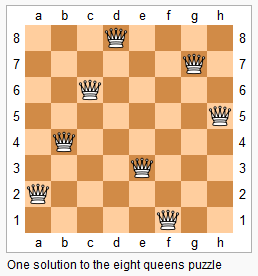
\includegraphics[width=.9\linewidth]{./pic/8-queens.png}
\caption{N-Queens}
\end{figure}

Given an integer n, return all distinct solutions to the n-queens puzzle.

Each solution contains a distinct board configuration of the n-queens' placement, where 'Q' and '.' both indicate a queen and an empty space respectively.

For example,

There exist two distinct solutions to the 4-queens puzzle:
\lstset{language=java,label= ,caption= ,numbers=none}
\begin{lstlisting}
[
 [".Q..",  // Solution 1
  "...Q",
  "Q...",
  "..Q."],

 ["..Q.",  // Solution 2
  "Q...",
  "...Q",
  ".Q.."]
]
\end{lstlisting}
\subsection{N-Queens II}
\label{sec-11-2-2}
Follow up for N-Queens problem.

Now, instead outputting board configurations, return the total number of distinct solutions.
\subsection{Sudoku Solver}
\label{sec-11-2-3}
Write a program to solve a Sudoku puzzle by filling the empty cells.

Empty cells are indicated by the character '.'.

You may assume that there will be only one unique solution.

\begin{figure}[htb]
\centering
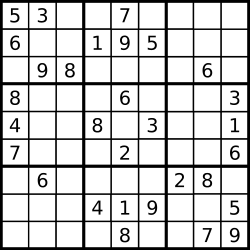
\includegraphics[width=.9\linewidth]{./pic/solveSudoku1.png}
\caption{Sudoku Solver 1}
\end{figure}

A sudoku puzzle\ldots{}

\begin{figure}[htb]
\centering
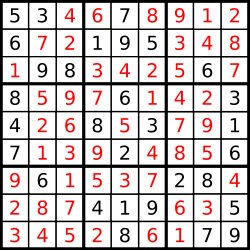
\includegraphics[width=.9\linewidth]{./pic/solveSudoku2.png}
\caption{Sudoku Solver 2}
\end{figure}
\ldots{}and its solution numbers marked in red.

\textbf{Tags:} Backtracking, Hash Table

\subsection{Word Search}
\label{sec-11-2-4}
Given a 2D board and a word, find if the word exists in the grid.

The word can be constructed from letters of sequentially adjacent cell, where "adjacent" cells are those horizontally or vertically neighboring. The same letter cell may not be used more than once.

For example,
\lstset{language=java,label= ,caption= ,numbers=none}
\begin{lstlisting}
Given board =
[
  ["ABCE"],
  ["SFCS"],
  ["ADEE"]
]
word = "ABCCED", -> returns true,
word = "SEE", -> returns true,
word = "ABCB", -> returns false.
\end{lstlisting}
\section{other Covered}
\label{sec-11-3}
\begin{itemize}
\item Same Tree
\ref{sec-4-1-8}
\item Symmetric Tree
\ref{sec-4-1-9}
\item Balanced Binary Tree
\ref{sec-4-1-10}
\item Validate Binary Search Tree
\ref{sec-4-3-1}
\item Convert Sorted List to Binary Search Tree
\ref{sec-3-2-8}
\item Convert Sorted Array to Binary Search Tree
\ref{sec-4-3-2}
\item Construct Binary Tree from Preorder and Inorder Traversal
\ref{sec-4-2-1}
\item Construct Binary Tree from Inorder and Postorder Traversal
\ref{sec-4-2-2}
\item Flatten Binary Tree to Linked List
\ref{sec-4-1-11}
\item Populating Next Right Pointers in Each Node
\ref{sec-4-4-6}
\item Populating Next Right Pointers in Each Node II
\ref{sec-4-1-12}
\item Sum Root to Leaf Numbers        
\ref{sec-4-4-7}
\item Path Sum
\ref{sec-4-4-3}
\item Path Sum II
\ref{sec-4-4-4}
\item Maximum Depth of Binary Tree
\ref{sec-4-4-2}
\item Recover Binary Search Tree
\ref{sec-4-1-7}
\item Clone Graph
\ref{sec-18-1-1}
\item Binary Tree Maximum Path Sum
\ref{sec-4-4-5}
\end{itemize}
\chapter{分治法 Divide and Conqure}
\label{sec-12}
\section{Medium}
\label{sec-12-1}
\subsection{Pow(x, n)}
\label{sec-12-1-1}
Implement pow(x, n).

\textbf{Tags:} Math, Binary Search

二分法, x$^{\text{n}}$ = x$^{\text{n/2}}$ × x$^{\text{n/2}}$ × x$^{\text{n\%2}}$

时间复杂度 O(logn), 空间复杂度 O(1).
\lstset{language=java,label= ,caption= ,numbers=none}
\begin{lstlisting}
public double myPower(double x, int n) {
    if (n == 0) return 1;
    double val = myPower(x, n / 2);
    if (n % 2 == 0) return val * val;
    else return val * val * x;
}

public double pow(double x, int n) {
    if (n < 0) return 1.0 / myPower(x, -n);
    else return myPower(x, n);
}
\end{lstlisting}

\subsection{Sqrt(x)}
\label{sec-12-1-2}
Implement int sqrt(int x).

Compute and return the square root of x.

\textbf{Tags:} Math, Binary Search

二分查找

时间复杂度 O(logn), 空间复杂度 O(1).
\lstset{language=java,label= ,caption= ,numbers=none}
\begin{lstlisting}
public int sqrt(int x) {
    int bgn = 0, end = 0;
    int mid = 0;
    int lastMid = 0;
    if (x < 2) return x;
    // end = x / 2;          // which one is better ?
    end = x / 2 < (int)Math.sqrt(Integer.MAX_VALUE) ?
        x / 2 + 1 : (int)Math.sqrt(Integer.MAX_VALUE);
    while (bgn <= end) {
        mid = bgn + (end - bgn) / 2;
        if (x / mid == mid)  // 不要用 x > mid * mid, 会溢出
            return mid;
        else if (x / mid > mid) {
            bgn = mid + 1;
            lastMid = mid;
        } else  // x / mid < mid
            end = mid - 1;
    }
    return lastMid;
}
\end{lstlisting}

\section{other Covered}
\label{sec-12-2}
\begin{itemize}
\item Majority Element
\ref{sec-1-4-1}
\item Maximum Subarray
\texttt{Maximum Subarray}
\item Merge K sorted List
\texttt{Merge K sorted List}
\end{itemize}
\chapter{贫心法 Greedy Search}
\label{sec-13}
\section{Medium}
\label{sec-13-1}
\subsection{Gas Station}
\label{sec-13-1-1}
There are N gas stations along a circular route, where the amount of gas at station i is gas[i].

You have a car with an unlimited gas tank and it costs cost[i] of gas to travel from station i to its next station (i+1). You begin the journey with an empty tank at one of the gas stations.

Return the starting gas station's index if you can travel around the circuit once, otherwise return -1.

Note:

The solution is guaranteed to be unique.

\subsection{Best Time to Buy and Sell Stock}
\label{sec-13-1-2}
Say you have an array for which the ith element is the price of a given stock on day i.

If you were only permitted to complete at most one transaction (ie, buy one and sell one share of the stock), design an algorithm to find the maximum profit.

贪心法, 分别找到价格最低和最高的一天, 低进高出, 注意最低的一天要在最高的一天之前。把原始价格序列变成差分序列, 本题也可以做是最大 m 子段和, m = 1。

时间复杂度 O(n), 空间复杂度 O(1).

\lstset{language=java,label= ,caption= ,numbers=none}
\begin{lstlisting}
public int maxProfit(int[] prices) {
    int lowest = Integer.MAX_VALUE;
    int maxProfit = 0;
    for (int i = 0; i < prices.length; i++) {
        if (prices[i] < lowest) lowest = prices[i];
        else maxProfit = Math.max(maxProfit, prices[i] - lowest);
    }
    return maxProfit;
}
\end{lstlisting}

\subsection{Best Time to Buy and Sell Stock II}
\label{sec-13-1-3}
Say you have an array for which the ith element is the price of a given stock on day i.

Design an algorithm to find the maximum profit. You may complete as many transactions as you like (ie, buy one and sell one share of the stock multiple times). However, you may not engage in multiple transactions at the same time (ie, you must sell the stock before you buy again).

贪心法, 低进高出, 把所有正的价格差价相加起来。把原始价格序列变成差分序列, 本题也可以做是最大 m 子段和, m = 数组长度。

\lstset{language=java,label= ,caption= ,numbers=none}
\begin{lstlisting}
public int maxProfit(int[] prices) {
    int result = 0;
    for (int i = 0; i < prices.length-1; i++) 
        result += (prices[i] < prices[i+1]) ? prices[i + 1] - prices[i] : 0;
    return result;
}
\end{lstlisting}

\subsection{Jump Game}
\label{sec-13-1-4}
Given an array of non-negative integers, you are initially positioned at the first index of the array.

Each element in the array represents your maximum jump length at that position.

Determine if you are able to reach the last index.

For example:

A = [2, 3, 1, 1, 4], return true.

A = [3, 2, 1, 0, 4], return false.

\section{Hard}
\label{sec-13-2}
\subsection{Jump Game II}
\label{sec-13-2-1}
Given an array of non-negative integers, you are initially positioned at the first index of the array.

Each element in the array represents your maximum jump length at that position.

Your goal is to reach the last index in the minimum number of jumps.

For example:

Given array A = [2,3,1,1,4]

The minimum number of jumps to reach the last index is 2. (Jump 1 step from index 0 to 1, then 3 steps to the last index.)
\subsection{Candy}
\label{sec-13-2-2}
There are N children standing in a line. Each child is assigned a rating value.

You are giving candies to these children subjected to the following requirements:

Each child must have at least one candy.

Children with a higher rating get more candies than their neighbors.

What is the minimum candies you must give?
\subsection{Wildcard Matching}
\label{sec-13-2-3}
Implement wildcard pattern matching with support for '?' and '*'.
\lstset{language=java,label= ,caption= ,numbers=none}
\begin{lstlisting}
'?' Matches any single character.
'*' Matches any sequence of characters (including the empty sequence).
\end{lstlisting}

The matching should cover the entire input string (not partial).

The function prototype should be:

bool isMatch(const char *s, const char *p)

Some examples:
\lstset{language=java,label= ,caption= ,numbers=none}
\begin{lstlisting}
isMatch("aa","a") → false
isMatch("aa","aa") → true
isMatch("aaa","aa") → false
isMatch("aa", "*") → true
isMatch("aa", "a*") → true
isMatch("ab", "?*") → true
isMatch("aab", "c*a*b") → false
\end{lstlisting}
\textbf{Tags:} Dynamic Programming, Backtracking, Greedy, String

\chapter{动态归划 Dynamic Programming}
\label{sec-14}
\section{Easy}
\label{sec-14-1}
\subsection{Climbing Stairs}
\label{sec-14-1-1}
You are climbing a stair case. It takes n steps to reach to the top.

Each time you can either climb 1 or 2 steps. In how many distinct ways
can you climb to the top?
\begin{enumerate}
\item O(n)
\label{sec-14-1-1-1}
\lstset{language=java,label= ,caption= ,numbers=none}
\begin{lstlisting}
public int climbStairs(int n) {
    int [] res = new int[n + 1];
    res[0] = 1; // 1 stair
    res[1] = 2; // 2 stair
    for (int i = 2; i < n; i++) 
        res[i] = res[i - 2] + res[i - 1];
    return res[n - 1];
}
\end{lstlisting}

Considering odd and even, 实现滚动数组
\lstset{language=java,label= ,caption= ,numbers=none}
\begin{lstlisting}
public int climbStairs(int n) {
    if(n <= 0) return 0;
    int [] stairs = {1, 2};
    for(int i = 2;i < n; i++)
        stairs[i % 2] = stairs[0] + stairs[1];
    return n % 2 == 0 ? stairs[1] : stairs[0];
}
\end{lstlisting}
\item O( log(n) )
\label{sec-14-1-1-2}

\url{https://oj.leetcode.com/discuss/11211/o-log-n-solution-with-matrix-multiplication}

Most solutions are DP with runtime O(n) and O(1) space, the only O(log(n)) solution so far is lucastan's using Binet's formula.

There actually is a matrix multiplication solution which also runs in O(log(n)). It basically calculates fibonacci numbers by power of matrix ((0, 1), (1, 1)) \^{} (n-1).

\lstset{language=java,label= ,caption= ,numbers=none}
\begin{lstlisting}
private int[][] pow(int[][] a, int n) {
    int[][] ret = {{1, 0}, {0, 1}};
    while (n > 0) {
        if ((n & 1) == 1) 
            ret = multiply(ret, a);
        n >>= 1;
        a = multiply(a, a);
    }
    return ret;
}

private int[][] multiply(int[][] a, int[][] b) {
    int[][] c = new int[2][2];
    for (int i = 0; i < 2; i++) 
        for (int j = 0; j < 2; j++) 
            c[i][j] = a[i][0] * b[0][j] + a[i][1] * b[1][j];
    return c;
}

public int climbStairs(int n) {
    int[][] a = {{0, 1}, {1, 1}};
    int[][] m = pow(a, n - 1);
    return m[0][1] + m[1][1];
}
\end{lstlisting}
\end{enumerate}
\section{Medium}
\label{sec-14-2}
\subsection{Unique Path}
\label{sec-14-2-1}
A robot is located at the top-left corner of a m x n grid (marked 'Start' in the diagram below).

The robot can only move either down or right at any point in time. The robot is trying to reach the bottom-right corner of the grid (marked 'Finish' in the diagram below).

How many possible unique paths are there?
\begin{figure}[htb]
\centering
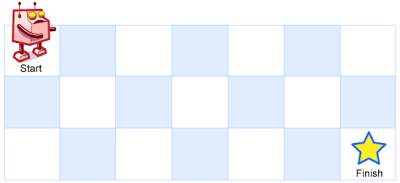
\includegraphics[width=.9\linewidth]{./pic/uniquePaths.png}
\caption{Unique Path}
\end{figure}

Above is a 3 x 7 grid. How many possible unique paths are there?

Note: m and n will be at most 100.

这里Note的含义是: 如果数值过大会溢出的。--《靖空间》

方法论总结:遇上新颖没见过的题目:
\begin{itemize}
\item 查看其特征;
\item 搜索大脑有什么熟悉的题目,可以套的,或者相似的可以退到出来的;
\item 罗列出来这些题目:全排列, 水槽,TwoSum,等等;
\item 搜索大脑里面有什么熟悉的算法;
\item 罗列出来:动态规划法,递归,回溯,二叉树遍历,贪心法,递归树,分治法,观察特征计算法,等等,肯定有可以套的算法的!
\item 最后选定算法解题;
\item 没有优化的算法,可以使用暴力法,先解决再说!
\end{itemize}

最后实在没招了,想办法让人提示,主要是提示用什么算法,能给个思路更好了,O(∩$_{\text{∩}}$)O\textasciitilde{}

\begin{enumerate}
\item 深搜, 递归法
\label{sec-14-2-1-1}

深搜,小集合可以过,大集合会超时;时间复杂度 O(n$^{\text{4}}$),空间复杂度 O(n);
\lstset{language=java,label= ,caption= ,numbers=none}
\begin{lstlisting}
public int uniquePaths(int m, int n) {
    if (m < 1 || n < 1) return 0;   // 终止条件
    if (m == 1 && n == 1) return 1; // 收敛条件
    return uniquePaths(m - 1, n) + uniquePaths(m, n - 1);
}
\end{lstlisting}
\item 备忘录法: 时间复杂度 O(n$^{\text{2}}$), 空间复杂度 O(n$^{\text{2}}$)
\label{sec-14-2-1-2}

给前面的深搜,加个缓存,就可以过大集合了。即备忘录法。
\lstset{language=java,label= ,caption= ,numbers=none}
\begin{lstlisting}
// 深搜 + 缓存,即备忘录法
// 时间复杂度 O(n^2), 空间复杂度 O(n^2)
class Solution {
    private int [][] f;    // 缓存

    public int dfs(int x, int y) {
        if (x < 1 || y < 1) return 0;   // 数据非法,终止条件
        if (x == 1 && y == 1) return 1; // 回到起点,收敛条件
        return getOrUpdate(x - 1, y) + getOrUpdate(x, y - 1);
    }

    public int getOrUpdate(int x, int y) {
        if (f[x][y] > 0) return f[x][y];
        else return f[x][y] = dfs(x, y);
    }

    public int uniquePaths(int m, int n) {        
        // 0 行和 0 列未使用
        f = new int[m + 1][n + 1]; // 缓存
        return dfs(m, n);
    }
}
\end{lstlisting}
\item 动态规划
\label{sec-14-2-1-3}

算法1的递归解法中,其实我们计算了很多重复的子问题,比如计算uniquePaths(4, 5) 和 uniquePaths(5, 3)时都要计算子问题uniquePaths(3,2),再者由于uniquePaths(m, n) = uniquePaths(n, m),这也使得许多子问题被重复计算了。

要保存子问题的状态,这样很自然的就想到了动态规划方法,设dp[i][j] = uniquePaths(i, j), 那么动态规划方程为:

动态方程: dp[i][j] = dp[i-1][j] + dp[i][j-1]

边界条件:dp[i][ 1 ] = 1, dp[ 1 ][j] = 1
\lstset{language=java,label= ,caption= ,numbers=none}
\begin{lstlisting}
public int uniquePaths(int m, int n) {
    if (m == 0 || n == 0) return 1;
    else if (m == 1 && n == 1) return 1;

    int [][] dp = new int[m][n];
    for (int i = 0; i < n; i++) 
        dp[0][i] = 1;
    for (int i = 0; i < m; i++)
        dp[i][0] = 1;
    dp[0][0] = 0;
    for (int i = 1; i < m; i++) 
        for (int j = 1; j < n; j++) 
            dp[i][j] = dp[i][j - 1] + dp[i - 1][j];
    return dp[m-1][n-1];
}
\end{lstlisting}

滚动数组
\lstset{language=java,label= ,caption= ,numbers=none}
\begin{lstlisting}
// 动规,滚动数组
// 时间复杂度 O(n^2), 空间复杂度 O(n)
int uniquePaths(int m, int n) {
    vector<int> f(n, 0);
    f[0] = 1;
    for (int i = 0; i < m; i++) {
        for (int j = 1; j < n; j++) {
            // 左边的 f[j], 表示更新后的 f[j], 与公式中的 f[i[[j] 对应
            // 右边的 f[j], 表示老的 f[j], 与公式中的 f[i-1][j] 对应
            f[j] = f[j - 1] + f[j];
        }
    }
    return f[n - 1];
}
\end{lstlisting}

\item 组合数 ( C$_{\text{m+n-2}}^{\text{m-1}}$ )
\label{sec-14-2-1-4}

一个 m 行, n 列的矩阵, 机器人从左上走到右下总共需要的步数是 m + n - 2, 其中向下走的步数是 m - 1, 因此问题变成了在 m + n - 2 个操作中, 选择 m–1 个时间点向下走, 选择方式有多少种。即C$_{\text{m+n-2}}^{\text{m-1}}$。这里需要注意的是求组合数时防止乘法溢出。
\lstset{language=java,label= ,caption= ,numbers=none}
\begin{lstlisting}
public int combination(int a, int b) {
    if (b > (a >>> 1)) b = a - b;
    long res = 1;
    for (int i = 1; i <= b ; i++) 
        res = res * (a - i + 1) / i;
    return (int)res;
}

public int uniquePaths(int m, int n) {
    return combination(m + n - 2, m - 1);
}
\end{lstlisting}
\end{enumerate}

\subsection{Unique Path with Obstacles}
\label{sec-14-2-2}
Follow up for "Unique Paths":

Now consider if some obstacles are added to the grids. How many unique paths would there be?

An obstacle and empty space is marked as 1 and 0 respectively in the grid.

For example, There is one obstacle in the middle of a 3x3 grid as illustrated below.
\lstset{language=java,label= ,caption= ,numbers=none}
\begin{lstlisting}
[
  [0,0,0],
  [0,1,0],
  [0,0,0]
]
\end{lstlisting}

The total number of unique paths is 2.

Note: m and n will be at most 100.
\begin{enumerate}
\item 备忘录法
\label{sec-14-2-2-1}
\lstset{language=java,label= ,caption= ,numbers=none}
\begin{lstlisting}
// LeetCode, Unique Paths II
// 深搜 + 缓存, 即备忘录法
class Solution {
public:
    int uniquePathsWithObstacles(vector<vector<int> > &obstacleGrid) {
        const int m = obstacleGrid.size();
        const int n = obstacleGrid[0].size();
        // 0 行和 0 列未使用
        this->f = vector<vector<int> >(m + 1, vector<int>(n + 1, 0));
        return dfs(obstacleGrid, m, n);
    }

private:
    vector<vector<int> > f;                    // 缓存
    int dfs(const vector<vector<int> > &obstacleGrid,
            int x, int y) {
        if (x < 1 || y < 1) return 0;         // 数据非法,终止条件

        if (obstacleGrid[x-1][y-1]) return 0; // (x,y) 是障碍
        if (x == 1 and y == 1) return 1;      // 回到起点,收敛条件
        return getOrUpdate(obstacleGrid, x - 1, y) +
                getOrUpdate(obstacleGrid, x, y - 1);
    }
    int getOrUpdate(const vector<vector<int> > &obstacleGrid,
                    int x, int y) {
        if (f[x][y] > 0) return f[x][y];
        else return f[x][y] = dfs(obstacleGrid, x, y);
    }
};
\end{lstlisting}
\item 动态规划
\label{sec-14-2-2-2}

与上一题类似, 但要特别注意第一列的障碍。在上一题中,第一列全部是1, 但是在这一题中不同,第一列如果某一行有障碍物,那么后面的行应该为 0。
\lstset{language=java,label= ,caption= ,numbers=none}
\begin{lstlisting}
public int uniquePathsWithObstacles(int[][] obstacleGrid) {
    int m = obstacleGrid.length;
    int n = obstacleGrid[0].length;
    if (m == 0 || n == 0) return 0;
    else if (obstacleGrid[0][0] == 1 || obstacleGrid[m - 1][n - 1] == 1) return 0;
    else if (m == 1 || n == 1) return obstacleGrid[m-1][n-1] == 1 ? 0 : 1;

    int [][] arr = new int[m][n];
    for (int i = 0; i < n; i++)
        if (obstacleGrid[0][i] == 1) {
            for (int j = i; j < n; j++) 
                arr[0][j] = 0;
            i = n;
        } else arr[0][i] = 1;

    for (int i = 0; i < m; i++)
        if (obstacleGrid[i][0] != 1)
            arr[i][0] = 1;
        else 
            for (int j = i; j < m; j++) {
                arr[j][0] = 0;
                i = m;
            }

    arr[0][0] = 0;
    for (int i = 1; i < m; i++) {
        for (int j = 1; j < n; j++) {
            if (obstacleGrid[i][j] == 1)
                arr[i][j] = 0;
            else 
                arr[i][j] = arr[i][j - 1] + arr[i - 1][j];
        }
    }
    return arr[m-1][n-1];
}
\end{lstlisting}
\end{enumerate}
\subsection{Minimum Path Sum}
\label{sec-14-2-3}
Given a m x n grid filled with non-negative numbers, find a path from top left to bottom right which minimizes the sum of all numbers along its path.

Note: You can only move either down or right at any point in time.

跟 Unique Paths (见 §10.2) 很类似。设状态为 f[i][j], 表示从起点 (0, 0) 到达 (i, j) 的最小路径和, 则状态转移方程为: 

转移方程: f[i][j] = min(f[i-1][j], f[i][j-1]) + grid[i][j]
\begin{enumerate}
\item 备忘录法
\label{sec-14-2-3-1}

代码应该可以再优化一下。
\lstset{language=java,label= ,caption= ,numbers=none}
\begin{lstlisting}
private int [][] f;

private int getOrUpdate(int [][] grid, int x, int y) {
    if (x < 0 || y < 0) return Integer.MAX_VALUE;
    if (f[x][y] >= 0) return f[x][y];
    else {
        f[x][y] = dfs(grid, x, y);
        return f[x][y];
    }
}

private int dfs(int [][] grid, int x, int y) {
    if (x < 0 || y < 0) return Integer.MAX_VALUE;
    if (x == 0 && y == 0) return grid[0][0];
    return Math.min(getOrUpdate(grid, x - 1, y),
                    getOrUpdate(grid, x, y - 1)) + grid[x][y];
}

public int minPathSum(int[][] grid) {
    int m = grid.length;
    int n = grid[0].length;
    f = new int[m][n];
    for (int i = 0; i < m; i++) 
        for (int j = 0; j < n; j++) 
            f[i][j] = -1;
    return dfs(grid, m - 1, n - 1);
}
\end{lstlisting}
\item 动态规划
\label{sec-14-2-3-2}
\lstset{language=java,label= ,caption= ,numbers=none}
\begin{lstlisting}
public int minPathSum(int[][] grid) {
    int m = grid.length;
    int n = grid[0].length;
    if (m == 0 || n == 0) return 0;

    int [][] f = new int[m][n];
    f[0][0] = grid[0][0];
    for (int i = 1; i < n; i++)
        f[0][i] = f[0][i - 1] + grid[0][i];
    for (int i = 1; i < m; i++)
        f[i][0] = f[i - 1][0] + grid[i][0];

    for (int i = 1; i < m; i++) 
        for (int j = 1; j < n; j++) 
            f[i][j] = Math.min(f[i][j - 1], f[i - 1][j]) + grid[i][j];
    return f[m-1][n-1];
}
\end{lstlisting}
\item 动态规划 + 滚动数组
\label{sec-14-2-3-3}
\end{enumerate}
\subsection{Unique Binary Search Tree}
\label{sec-14-2-4}
Given n, how many structurally unique BST's (binary search trees) that store values 1\ldots{}n?

For example, Given n = 3, there are a total of 5 unique BST's.
\lstset{language=java,label= ,caption= ,numbers=none}
\begin{lstlisting}
1         3     3      2      1
 \       /     /      / \      \
  3     2     1      1   3      2
 /     /       \                 \
2     1         2                 3
\end{lstlisting}

如果把上例的顺序改一下,就可以看出规律了。《水中的鱼》
\lstset{language=java,label= ,caption= ,numbers=none}
\begin{lstlisting}
1           1                   2                   3           3
 \           \                 / \                 /           / 
  3           2               1   3               2           1
 /             \                                 /             \
2               3                               1               2
\end{lstlisting}

比如,以1为根的树有几个,完全取决于有二个元素的子树有几种。同理,2为根的子树取决于一个元素的子树有几个。以3为根的情况,则与1相同。

定义Count[i] 为以[0,i]能产生的Unique Binary Tree的数目,

如果数组为空,毫无疑问,只有一种BST,即空树, Count[ 0 ] =1

如果数组仅有一个元素\{1\},只有一种BST,单个节点, Count[ 1 ] = 1

如果数组有两个元素\{1,2\}, 那么有如下两种可能
\lstset{language=java,label= ,caption= ,numbers=none}
\begin{lstlisting}
1                2
 \              /
  2            1
Count[2] = Count[0] * Count[1]   ( 1 为根的情况 )
         + Count[1] * Count[0]   ( 2 为根的情况 )
\end{lstlisting}

再看一遍三个元素的数组,可以发现BST的取值方式如下:
\lstset{language=java,label= ,caption= ,numbers=none}
\begin{lstlisting}
Count[3] = Count[0]*Count[2]  ( 1 为根的情况 )
         + Count[1]*Count[1]  ( 2 为根的情况 )
         + Count[2]*Count[0]  ( 3 为根的情况 )
\end{lstlisting}

所以,由此观察,当数组为 1, 2, 3, \ldots{}, n 时,基于以下原则的构建的 BST 树具有唯一性:以 i 为根节点的树,其左子树由 [1, i-1] 构成,其右子树由 [i+1, n] 构成。

可以得出Count的递推公式为

Count(i) = $\sum$$_{\text{k = 1}}^{\text{i}}$ Count(k - 1) * Count(i - k) 

问题至此划归为一维动态规划。
\lstset{language=java,label= ,caption= ,numbers=none}
\begin{lstlisting}
public int numTrees(int n) {
    int [] cnt = new int[n + 1];
    cnt[0] = 1; // empty element
    cnt[1] = 1; // one element
    for (int i = 2; i <= n ; i++) 
        for (int j = 0; j < i; j++) 
            cnt[i] += cnt[j]*cnt[i - 1 - j];
    return cnt[n];
}
\end{lstlisting}
\subsection{Unique Binary Search Tree II}
\label{sec-14-2-5}
Given n, generate all structurally unique BST's (binary search trees) that store values 1\ldots{}n.

For example,

Given n = 3, your program should return all 5 unique BST's shown below.
\lstset{language=java,label= ,caption= ,numbers=none}
\begin{lstlisting}
1         3     3      2      1
 \       /     /      / \      \
  3     2     1      1   3      2
 /     /       \                 \
2     1         2                 3
\end{lstlisting}
\lstset{language=java,label= ,caption= ,numbers=none}
\begin{lstlisting}
public List<TreeNode> helper(int bgn, int end) {
    List<TreeNode> res = new ArrayList<TreeNode>();
    if (bgn > end) {
        res.add(null);  // important
        return res;
    }

    List<TreeNode> left = null;
    List<TreeNode> right = null;
    TreeNode root = null;
    for (int i = bgn; i <= end ; i++) {
        left = helper(bgn, i - 1);
        right = helper(i + 1, end);
        for (int j = 0; j < left.size(); j++) {
            for (int k = 0; k < right.size(); k++) {
                root = new TreeNode(i);
                root.left = left.get(j);
                root.right = right.get(k);
                res.add(root);
                root = null;
            }
        }
        left = null;
        right = null;
    }
    return res;
}

public List<TreeNode> generateTrees(int n) {
    return helper(1, n);
}
\end{lstlisting}
\subsection{Maximum Sum Subarray}
\label{sec-14-2-6}
Find the contiguous subarray within an array (containing at least one number) which has the largest sum.

For example, given the array [-2, 1, -3, 4, -1, 2, 1, -5, 4], 

the contiguous subarray [4, -1, 2, 1] has the largest sum = 6.

click to show more practice.

\textbf{More practice:}

If you have figured out the O(n) solution, try coding another solution using the divide and conquer approach, which is more subtle.

\textbf{Tags:} Divide and Conquer, Array, Dynamic Programming

分析:

最大连续子序列和,非常经典的题。

当我们从头到尾遍历这个数组的时候, 对于数组里的一个整数, 它有几种选择呢? 它只有两种选择: 1、加入之前的 SubArray;  2. 自己另起一个 SubArray。那什么时候会出现这两种情况呢?

\begin{itemize}
\item 如果之前 SubArray 的总体和大于 0 的话, 我们认为其对后续结果是有贡献的。这种情况下我们选择加入之前的 SubArray

\item 如果之前 SubArray 的总体和为 0 或者小于 0 的话, 我们认为其对后续结果是没有贡献, 甚至是有害的(小于 0 时)。这种情况下我们选择以这个数字开始, 另起一个 SubArray。
\end{itemize}

设状态为 f[j], 表示以 S[j] 结尾的最大连续子序列和, 则状态转移方程如下:
\lstset{language=java,label= ,caption= ,numbers=none}
\begin{lstlisting}
f[j] = max (f[j-1] + S[j], S[j]) , 其中 1 ≤ j ≤ n
target = max (f[j]) , 其中 1 ≤ j ≤ n
\end{lstlisting}

解释如下:

情况一, S[j]不独立, 与前面的某些数组成一个连续子序列, 则最大连续子序列和为 f[j-1] + S[j]。

情况二, S[j] 独立划分成为一段, 即连续子序列仅包含一个数 S[j], 则最大连续子序列和为S[j]。

其他思路:
\begin{itemize}
\item 思路 2: 直接在 i 到 j 之间暴力枚举, 复杂度是 O(n$^{\text{3}}$)
\item 思路 3: 处理后枚举, 连续子序列的和等于两个前缀和之差, 复杂度 O(n$^{\text{2}}$)。
\item 思路 4: 分治法, 把序列分为两段, 分别求最大连续子序列和, 然后归并, 复杂度 O( n*(log(n)) )
\item 思路 5: 把思路 2 O(n$^{\text{2}}$) 的代码稍作处理, 得到 O(n) 的算法
\item 思路 6: 当成 M = 1 的最大 M 子段和
\end{itemize}
\begin{enumerate}
\item 动态规划: 时间复杂度 O(n), 空间复杂度 O(1)
\label{sec-14-2-6-1}
\lstset{language=java,label= ,caption= ,numbers=none}
\begin{lstlisting}
public int maxSubArray(int[] a) {
    int result = Integer.MIN_VALUE, f = 0;
    for (int i = 0; i < a.length; i++) {
        f = Math.max(f + a[i], a[i]);
        result = Math.max(result, f);
    }
    return result;
}
\end{lstlisting}
\item 思路 5: 时间复杂度 O(n),空间复杂度 O(n)
\label{sec-14-2-6-2}
\lstset{language=java,label= ,caption= ,numbers=none}
\begin{lstlisting}
public int maxSubArray(int[] a) {
    int result, curMin;
    int [] sum = new int[a.length + 1];
    sum[0] = 0;
    result = Integer.MIN_VALUE;
    curMin = sum[0];
    for (int i = 1; i <= a.length; i++) 
        sum[i] = sum[i - 1] + a[i - 1];
    for (int i = 1; i <= a.length; i++) {
        result = Math.max(result, sum[i] - curMin);
        curMin = Math.min(curMin, sum[i]);
    }
    return result;
}
\end{lstlisting}
\end{enumerate}
\subsection{Maximum Product Subarray}
\label{sec-14-2-7}
Find the contiguous subarray within an array (containing at least one number) which has the largest product.

For example, given the array [2, 3, -2, 4], 

the contiguous subarray [2, 3] has the largest product = 6.

这道题跟\ref{sec-14-2-6}模型上和思路上都比较类似,还是用一维动态规划中的“局部最优和全局最优法”。

这里的区别是维护一个局部最优不足以求得后面的全局最优,这是由于乘法的性质不像加法那样,累加结果只要是正的一定是递增,乘法中有可能现在看起来小的一个负数,后面跟另一个负数相乘就会得到最大的乘积。

不过事实上也没有麻烦很多,我们只需要在维护一个局部最大的同时,在维护一个局部最小,这样如果下一个元素遇到负数时,就有可能与这个最小相乘得到当前最大的乘积和,这也是利用乘法的性质得到的。

来自《Code Ganker征服代码》

\lstset{language=java,label= ,caption= ,numbers=none}
\begin{lstlisting}
public int maxProduct(int[] a) {
    int n = a.length;
    int maxLocal = a[0];
    int minLocal = a[0];
    int res = a[0];
    for (int i = 1; i < n; i++) {
        int tmp = maxLocal;
        maxLocal = Math.max(Math.max(maxLocal * a[i], a[i]),
                            Math.max(minLocal * a[i], a[i]));
        minLocal = Math.min(Math.min(a[i], a[i] * tmp),
                            Math.min(a[i], a[i] * minLocal));
        res = Math.max(res, maxLocal);
    }
    return res; 
}
\end{lstlisting}
\subsection{Decode Ways, bug\textasciitilde{}~!!}
\label{sec-14-2-8}
A message containing letters from A-Z is being encoded to numbers using the following mapping:
\lstset{language=java,label= ,caption= ,numbers=none}
\begin{lstlisting}
'A' -> 1
'B' -> 2
...
'Z' -> 26
\end{lstlisting}

Given an encoded message containing digits, determine the total number of ways to decode it.

For example,

Given encoded message "12", it could be decoded as "AB" (1 2) or "L" (12).

The number of ways decoding "12" is 2.

参考Climb stairs, \ref{sec-14-1-1}

最原始型的follow、控制logic:
\lstset{language=java,label= ,caption= ,numbers=none}
\begin{lstlisting}
public int numDecodings(String s) {
    if (s == null || s.length() == 0) return 0;
    else if (s.charAt(0) == '0') return 0;
    else if (s.length() == 1) return 1;
    else if (s.length() >= 2 && s.charAt(0) - '0' > 2 && s.charAt(1) == '0') return 0;

    int j = 0; // idx for s
    char c;    // char at pos j
    int [] res = new int[s.length()];
    res[0] = 1;
    res[1] = 1;
    if (s.charAt(1) != '0'
        && ( (s.charAt(0) == '1'
              || (s.charAt(0) == '2') && s.charAt(1) - '0' < 7)))
        res[1] = 2;

    for (int i = 2; i < s.length(); i++) {
        c = s.charAt(i);
        if (c != '0')
            res[i] += res[i - 1]; // separate dijit // except '0', NO, 10, 20 ok

        switch (c) {
        case '0':
            if (s.charAt(i - 1) == '1' || s.charAt(i - 1) == '2')
                if (s.charAt(i - 2) == '1' || s.charAt(i - 2) == '2')
                    res[i] = res[i - 2];     // 110 = 1 10, ... 11 0, NO~!
                else
                    res[i] = res[i - 1]; 
            else return 0;
            break;
        case '7':     // 17, 18, 19
        case '8':
        case '9':
            if (s.charAt(i - 1) == '1')
                res[i] += res[i - 2];
            break;
        default:     // 1, 2, 3, 4, 5, 6: Individual, 1-pre, 2-pre, 11, 21, 12, 22 ...
            if (s.charAt(i - 1) == '1' || s.charAt(i - 1) == '2')
                res[i] += res[i - 2];
            break;
        }
    }
    return res[s.length() - 1];
}
\end{lstlisting}
\begin{enumerate}
\item 动态规划, 时间复杂度 O(n), 空间复杂度 O(1), java v m bug \verb,~~,!!!!
\label{sec-14-2-8-1}

模拟pdf c++版大牛精华版代码: 
\lstset{language=java,label= ,caption= ,numbers=none}
\begin{lstlisting}
// my Java version code has bug here, fix it later ~~~
public int numDecodings(String s) {
    if (s == null || s.length() == 0 || s.charAt(0) == '0') return 0;
    int prev = 0;
    int curr = 1;
    int tmp = 0;
    for (int i = 1; i <= s.length() ; i++) {
        if (s.charAt(i - 1) == '0') curr = 0;
        if (i < 2 || s.charAt(i - 2) != '1' ||
            (s.charAt(i - 2) == '2' && s.charAt(i - 1) <= '6'))
            prev = 0;
        tmp = curr;
        curr = prev + curr;
        prev = tmp;
    }
    return curr;
}
\end{lstlisting}
\end{enumerate}

\subsection{Triangle}
\label{sec-14-2-9}
Given a triangle, find the minimum path sum from top to bottom. Each step you may move to adjacent numbers on the row below.

For example, given the following triangle
\lstset{language=java,label= ,caption= ,numbers=none}
\begin{lstlisting}
[
     [2],
    [3,4],
   [6,5,7],
  [4,1,8,3]
]
\end{lstlisting}

The minimum path sum from top to bottom is 11 (i.e., 2 + 3 + 5 + 1 = 11).

Note: Bonus point if you are able to do this using only O(n) extra space, where n is the total number of rows in the triangle.
\begin{enumerate}
\item 自顶向下: 时间复杂度是O(n$^{\text{2}}$), 空间复杂度是O(n)
\label{sec-14-2-9-1}

这是一道动态规划的题目,求一个三角形二维数组从顶到低端的最小路径和。思路是维护到某一个元素的最小路径和,那么在某一个元素i,j的最小路径和就是它上层对应的相邻两个元素的最小路径和加上自己的值,递推式是

sum[i][j] = min(sum[i-1][j-1],sum[i-1][j]) + triangle[i][j]。

最后扫描一遍最后一层的路径和,取出最小的即可。每个元素需要维护一次,总共有 1+2+\ldots{}+n = n*(n+1)/2 个元素,所以时间复杂度是O(n$^{\text{2}}$)。而空间上每次只需维护一层即可(因为当前层只用到上一层的元素),所以空间复杂度是O(n)。

来自《Code Ganker征服代码》
\lstset{language=java,label= ,caption= ,numbers=none}
\begin{lstlisting}
public int minimumTotal(ArrayList<ArrayList<Integer>> triangle) {  
    if(triangle == null || triangle.size() == 0)  
        return 0;  
    if(triangle.size() == 1)  
        return triangle.get(0).get(0);

    int[] dp = new int[triangle.size()];  
    dp[0] = triangle.get(0).get(0);  
    for(int i = 1; i < triangle.size(); i++) {  
        dp[i] = dp[i - 1] + triangle.get(i).get(i);  
        for(int j = i - 1 ; j >= 1; j--)  
            dp[j] = (dp[j] < dp[j-1] ? dp[j] : dp[j - 1]) + triangle.get(i).get(j);  
        dp[0] = dp[0] + triangle.get(i).get(0);  
    }

    int minimum = dp[0];  
    for(int i = 1; i < dp.length; i++) 
        if (dp[i] < minimum)
            minimum = dp[i];  
    return minimum;  
}
\end{lstlisting}

上述代码实现时要注意每层第一个和最后一个元素特殊处理一下。
\item 自底向上:
\label{sec-14-2-9-2}

换个角度考虑一下,如果这道题不自顶向下进行动态规划,而是放过来自底向上来规划,递归式只是变成下一层对应的相邻两个元素的最小路径和加上自己的值,原理和上面的方法是相同的,这样考虑到优势在于不需要最后对于所有路径找最小的,而且第一个元素和最后元素也不需要单独处理了,所以代码简洁了很多。
\lstset{language=java,label= ,caption= ,numbers=none}
\begin{lstlisting}
public int minimumTotal(List<List<Integer>> triangle) {
    List<Integer> res = new ArrayList<Integer>(triangle.get(triangle.size() - 1));
    for (int i = triangle.size() - 2; i >= 0 ; i--) 
        for (int j = 0; j <= i ; j++) 
            res.set(j, Math.min(res.get(j), res.get(j + 1))
                    + triangle.get(i).get(j));
    return res.get(0);
}
\end{lstlisting}
\end{enumerate}
\subsection{Word Break}
\label{sec-14-2-10}
Given a string s and a dictionary of words dict, determine if s can be segmented into a space-separated sequence of one or more dictionary words.

For example, given
\lstset{language=java,label= ,caption= ,numbers=none}
\begin{lstlisting}
s = "leetcode",
dict = ["leet", "code"].
Return true because "leetcode" can be segmented as "leet code".
\end{lstlisting}

设状态为 f(i),表示 s[0,i] 是否可以分词,则状态转移方程为

转移方程: f (i) = any$_{\text{of}}$ ( f(j) \&\& s[j+1, i] ∈ dict ), 0 ≤ j < i
\begin{enumerate}
\item 深搜: 时间复杂度 O(2$^{\text{n}}$),空间复杂度 O(n)
\label{sec-14-2-10-1}

OJ 超时。
\lstset{language=java,label= ,caption= ,numbers=none}
\begin{lstlisting}
public boolean helper(String s, int i, Set<String> dict) {
    int n = s.length();
    if (i >= n) return false;
    int j = i;
    while (j < n) {
        while (j < n && !dict.contains(s.substring(i, j + 1))) j++;
        if (j == n) return false;
        if (helper(s, j + 1, dict) == true) return true;
        j++;
    }
    return false;
}

public boolean wordBreak(String s, Set<String> dict) {
    if (dict.contains(s)) return true;
    if (s == null || s.length() == 0) return false;
    return helper(s, 0, dict);
}
\end{lstlisting}
\item 动态规划:
\label{sec-14-2-10-2}
\lstset{language=java,label= ,caption= ,numbers=none}
\begin{lstlisting}
public boolean wordBreak(String s, Set<String> dict) {
    if (dict.contains(s)) return true;
    boolean [] dp = new boolean[s.length()];
    for (int i = 0; i < s.length(); i++) 
        dp[i] = false;

    for (int i = 0; i < s.length(); i++)
        for (int j = i; j >= 0; j--) {
            String tmp = new String(s.substring(j, i+1));
            if (dict.contains(tmp))
                if ((j == 0) || (j >= 1 && dp[j-1])) {
                    dp[i] = true;
                    break;
                }
        }
    return dp[s.length()-1];
}
\end{lstlisting}
\end{enumerate}

\section{Hard}
\label{sec-14-3}
\subsection{Best Time to Buy and Sell Stock III}
\label{sec-14-3-1}
Say you have an array for which the ith element is the price of a given stock on day i.

Design an algorithm to find the maximum profit. You may complete at most two transactions.

Note: You may not engage in multiple transactions at the same time (ie, you must sell the stock before you buy again).

设状态 f(i), 表示区间[0, i](0 ≤ i ≤ n−1) 的最大利润, 状态 g(i), 表示区间[i, n−1](0 ≤ i ≤ n−1)的最大利润, 则最终答案为 max\{ f(i) + g(i) \}, 0 ≤ i ≤ n−1。

允许在一天内买进又卖出,相当于不交易,因为题目的规定是最多两次,而不是一定要两次。

将原数组变成差分数组, 本题也可以看做是最大 m 子段和, m = 2.

\lstset{language=java,label= ,caption= ,numbers=none}
\begin{lstlisting}
public int maxProfit(int[] prices) {
    if (prices.length < 2) return 0; 
    int [] past = new int[prices.length];
    int [] futu = new int[prices.length];
    int result = 0;
    for (int i = 1, valley = prices[0]; i < prices.length; i++) {
        valley = Math.min(valley, prices[i]);
        past[i] = Math.max(past[i - 1], prices[i]-valley);
    }
    for (int i = prices.length-2, peak = prices[prices.length-1]; i >= 0 ; i--) {
        peak = Math.max(peak, prices[i]);
        futu[i] = Math.max(futu[i+1], peak-prices[i]);
        result = Math.max(result, past[i] + futu[i]);
    }
    return result;
}
\end{lstlisting}

\subsection{Coins in a Line}
\label{sec-14-3-2}

\subsection{Maximal Rectangle}
\label{sec-14-3-3}
Given a 2D binary matrix filled with 0's and 1's, find the largest rectangle containing all ones and return its area.

\textbf{Tags:} Array Hash Table Stack Dynamic Programming
\begin{enumerate}
\item 栈: O(n)
\label{sec-14-3-3-1}
这是一道非常综合的题目,要求在0-1矩阵中找出面积最大的全1矩阵。刚看到这道题会比较无从下手,brute force就是对于每个矩阵都看一下,总共有m(m+1)/2*n(n+1)/2个子矩阵(原理跟字符串子串类似,字符串的子串数有n(n+1)/2,只是这里是二维情形,所以是两个相乘),复杂度相当高,肯定不是面试官想要的答案,就不继续想下去了。

这道题的解法灵感来自于Largest Rectangle in Histogram这道题,假设我们把矩阵沿着某一行切下来,然后把切的行作为底面,将自底面往上的矩阵看成一个直方图(histogram)。直方图的中每个项的高度就是从底面行开始往上1的数量。根据Largest Rectangle in Histogram我们就可以求出当前行作为矩阵下边缘的一个最大矩阵。接下来如果对每一行都做一次Largest Rectangle in Histogram,从其中选出最大的矩阵,那么它就是整个矩阵中面积最大的子矩阵。
算法的基本思路已经出来了,剩下的就是一些节省时间空间的问题了。

我们如何计算某一行为底面时直方图的高度呢? 如果重新计算,那么每次需要的计算数量就是当前行数乘以列数。然而在这里我们会发现一些动态规划的踪迹,如果我们知道上一行直方图的高度,我们只需要看新加进来的行(底面)上对应的列元素是不是0,如果是,则高度是0,否则则是上一行直方图的高度加1。利用历史信息,我们就可以在线行时间内完成对高度的更新。我们知道,Largest Rectangle in Histogram的算法复杂度是O(n)。所以完成对一行为底边的矩阵求解复杂度是O(n+n)=O(n)。接下来对每一行都做一次,那么算法总时间复杂度是O(m*n)。

空间上,我们只需要保存上一行直方图的高度 O(n),加上Largest Rectangle in Histogram中所使用的空间O(n),所以总空间复杂度还是O(n)。

\lstset{language=java,label= ,caption= ,numbers=none}
\begin{lstlisting}
private int largestRectangleArea(int[] height) {
    Stack<Integer> s = new Stack<Integer>();
    int [] hnew = new int[height.length + 1];
    hnew = Arrays.copyOf(height, height.length + 1);
    int res = 0; 
    int tmp;     
    int left;
    for (int i = 0; i <= height.length; i++) {
        if (s.isEmpty() || hnew[i] > hnew[s.peek()]) s.push(i);
        else {
            tmp = s.pop();
            res = Math.max(res, hnew[tmp] * 
                           (s.isEmpty() ? i : i - s.peek() - 1));
            i--;
        }
    }
    return res;
}

public int maximalRectangle(char[][] matrix) {
    if (matrix == null || matrix.length == 0 || matrix[0].length == 0) return 0;
    int [] h = new int[matrix[0].length];
    int res = 0;     // record max area
    for (int i = 0; i < matrix.length; i++) {
        for (int j = 0; j < matrix[0].length; j++) 
            h[j] = matrix[i][j] == '0' ? 0 : h[j] + 1;
        res = Math.max(res, largestRectangleArea(h));
    }
    return res;
}
\end{lstlisting}
\item 动态规划:
\label{sec-14-3-3-2}

一般一个题目我首先会想想怎么暴力解决,比如这一题,可以枚举出所有的矩形,求出其中的面积最大者,那么怎么枚举呢,如果分别枚举矩形的宽度和高度,这样还得枚举矩形的位置,复杂度至少为O(n$^{\text{4}}$) (计算复杂度是我们把matrix的行、列长度都泛化为n,下同),我们可以枚举矩形左上角的位置,那么知道了矩形左上角的位置,怎么计算以某一点为左上角的矩形的最大面积呢?举例如下,下面的矩阵我们以(0,0)为矩形的左上角:
\lstset{language=java,label= ,caption= ,numbers=none}
\begin{lstlisting}
1 1 1 1 0 0
1 1 1 0 1 1
1 0 1 0 1 1
0 1 1 1 1 1
1 1 1 1 1 1
\end{lstlisting}

矩形高度是1时,宽度为第一行中从第一个位置起连续的1的个数,为4,面积为4 * 1=4

矩形高度是2时,第二行从第一个位置起连续1的个数是3,宽度为min(3,4)=3,面积为3*2=6

矩形高度为3时,第三行从第一个位置起连续1的个数是1,宽度为min(1,3)=1,面积为1*3=3

矩形高度为4时,第四行从第一个位置起连续1的个数是0,宽度为min(0,1)=0,面积为0*4=0

后面的行就不用计算了,因为上一行计算的宽度是0,下面所有宽度都是0

因此以(0,0)为左上角的矩形的最大面积是6,计算以某一点为左上角的矩形的最大面积复杂度是O(n)。

注意到上面我们用到了信息“从某一行某个位置开始连续的1的个数”,这个我们可以通过动态规划求得:设dp[i][j]是从点(i,j)开始,这一行连续1的个数,动态规划方程如下:

初始条件:
\begin{itemize}
\item dp[i][n-1] = (matrix[i][n-1] == '1') (n是matrix的列数)
\item dp[i][j] = (matrix[i][j] == '1') ?  1 + dp[i][j + 1] : 0 (从方程看出我们应该从每一行的后往前计算)
\end{itemize}
计算dp复杂度O(n$^{\text{2}}$),枚举左上角位置以及计算以该位置为左上角的矩形最大面积复杂度是O(n$^{\text{2}}$*n)=O(n$^{\text{3}}$),总的复杂度是O(n$^{\text{3}}$)

这个算法还可以优化,枚举到某个点时我们可以假设该点右下方全是1,得到一个假设最大面积,如果这个面积比当前计算好的面积还要小,该点就可以直接跳过;在上面计算以某点为左上角的矩形面积时,也可以剪枝,剪枝方法同上。《JustDoIT》
\lstset{language=java,label= ,caption= ,numbers=none}
\begin{lstlisting}
public int maximalRectangle(char[][] matrix) {
    if (matrix == null || matrix.length == 0 || matrix[0].length == 0) return 0;
    int m = matrix.length;
    int n = matrix[0].length;
    int [][] dp = new int[m][n];
    int res = 0;
    int width = 0;
    for (int i = 0; i < m; i++) 
        dp[i][n - 1] = matrix[i][n - 1] == '1' ? 1 : 0;
    for (int i = 0; i < m; i++) 
        for (int j = n - 2; j >= 0; j--) 
            if (matrix[i][j] == '1')
                dp[i][j] = dp[i][j + 1] + 1;
    for (int i = 0; i < m; i++) // 以每个点作为矩形的左上角计算所得的最大矩形面积
        for (int j = 0; j < n; j++) {
            if ((n - j) * (m - i) <= res)
                break;          // 剪枝,column-j 是最大宽度,row-i 是最大高度
            width = dp[i][j];
            for (int k = i; k < m && width > 0; k++) {
                if (width * (m - i) <= res)
                    break;    // 剪枝,row-i 是以点 (i,j) 为左上角的矩形的最大高度
                if (width > dp[k][j])
                    width = dp[k][j]; //矩形宽度要取从第 i 行到第 k 行宽度的最小值
                res = Math.max(res, width * (k - i + 1));
            }
        }
    return res;
}
\end{lstlisting}
\end{enumerate}

\subsection{Edit Distance}
\label{sec-14-3-4}
Given two words word1 and word2, find the minimum number of steps required to convert word1 to word2. (each operation is counted as 1 step.)

You have the following 3 operations permitted on a word:

a) Insert a character

b) Delete a character

c) Replace a character

设状态为 f[i][j], 表示 A[0, i] 和 B[0, j] 之间的最小编辑距离。设 A[0, i] 的形式是 str1c, B[0, j] 的形式是 str2d, 

一. 如果 c == d, 则 f[i][j] = f[i-1][j-1];

二. 如果 c != d,

(a) 如果将 c 替换成 d, 则~ ~ ~ ~ ~ ~ f[i][j] = f[i-1][j-1] + 1;

(b) 如果在 c 后面添加一个 d, 则~ f[i][j] = f[i][j-1] + 1;

(c) 如果将 c 删除, 则~ ~ ~ ~ ~ ~ ~ ~ ~ f[i][j] = f[i-1][j] + 1;

\begin{enumerate}
\item 动态规划:时间复杂度 O(n*m), 空间复杂度 O(n*m)。
\label{sec-14-3-4-1}
\lstset{language=java,label= ,caption= ,numbers=none}
\begin{lstlisting}
public int minDistance(String s, String t) {
    int m = s.length();
    int n = t.length();
    int [][] res = new int[m + 1][n + 1];
    for (int i = 0; i <= m; i++)
        res[i][0] = i;
    for (int i = 0; i <= n; i++)
        res[0][i] = i;
    for (int i = 1; i <= m; i++) 
        for (int j = 1; j <= n; j++) 
            if (s.charAt(i - 1) == t.charAt(j - 1))
                res[i][j] = res[i - 1][j - 1];
            else 
                res[i][j] = Math.min(Math.min(res[i - 1][j], res[i][j - 1]),
                                     Math.min(res[i - 1][j],
                                              res[i - 1][j - 1])) + 1;
    return res[m][n];
}
\end{lstlisting}
\item 动态规划 + 滚动数组:
\label{sec-14-3-4-2}
\end{enumerate}

\subsection{Distinct Subsequence}
\label{sec-14-3-5}
Given a string S and a string T, count the number of distinct subsequences of T in S.

A subsequence of a string is a new string which is formed from the original string by deleting some (can be none) of the characters without disturbing the relative positions of the remaining characters. (ie, "ACE" is a subsequence of "ABCDE" while "AEC" is not).

Here is an example:

S = "rabbbit", T = "rabbit"

Return 3.

设状态为 f(i, j), 表示 T[0, j] 在 S[0, i] 里出现的次数。首先, 无论 S[i] 和 T[j] 是否相等, 

若不使用 S[i], 则~ ~ ~ ~ ~ ~ ~ ~ ~ ~ ~ ~ ~ f(i, j) = f(i-1, j); 

若 S[i] == T[j], 则可以使用 S[i], 则 f(i, j) = f(i-1, j) + f(i-1, j-1)。

\lstset{language=java,label= ,caption= ,numbers=none}
\begin{lstlisting}
public int numDistinct(String s, String t) {
    if (s == null || s.length() == 0) return 0;
    int m = s.length();
    int n = t.length();
    int [][] res = new int[m + 1][n + 1];
    for (int i = 0; i <= m; i++) 
        res[i][0] = 1;
    for (int i = 1; i <= m; i++) {
        for (int j = 1; j <= n; j++) {
            if (s.charAt(i - 1) == t.charAt(j - 1))
                res[i][j] = res[i - 1][j] + res[i - 1][j - 1];
            else
                res[i][j] = res[i - 1][j];
        }
    }
    return res[m][n];
}
\end{lstlisting}

滚动数组: 时间复杂度 O(m*n), 空间复杂度 O(n)
\lstset{language=java,label= ,caption= ,numbers=none}
\begin{lstlisting}
public int numDistinct(String s, String t) {
    if (s == null || s.length() == 0) return 0;
    int m = s.length();
    int n = t.length();
    int [] res = new int[n + 1];
    res[0] = 1;
    for (int i = 0; i < m; i++) 
        for (int j = n - 1; j >= 0; j--) 
            res[j + 1] += s.charAt(i) == t.charAt(j) ? res[j] : 0;
    return res[n];
}
\end{lstlisting}

\subsection{Palindrome Partitioning II}
\label{sec-14-3-6}
Given a string s, partition s such that every substring of the partition is a palindrome.

Return the minimum cuts needed for a palindrome partitioning of s.

For example, 
\lstset{language=java,label= ,caption= ,numbers=none}
\begin{lstlisting}
given s = "aab",
Return 1 since the palindrome partitioning ["aa","b"] could be produced using 1 cut.
\end{lstlisting}

\begin{enumerate}
\item 思路1:leetcode online
\label{sec-14-3-6-1}

忘记从线上哪个贴子看的了,根据回文可能有的两种特性,奇数长度回文和偶数长度回文,进行一维dp的判断。
\lstset{language=java,label= ,caption= ,numbers=none}
\begin{lstlisting}
public int minCut(String s) {
    int n = s.length();
    int [] dp = new int[n + 1];
    for (int i = 0; i <= n ; i++) // initiate
        dp[i] = i - 1;
    for (int i = 0; i < n; i++) {
        // s[i - j] == s[i + j], aba
        for (int j = 0; i - j >= 0 && i + j <= n - 1 && s.charAt(i - j) == s.charAt(i + j); j++)
            dp[i + j + 1] = Math.min(dp[i - j] + 1, dp[i + j + 1]);
        // s[i - j] == s[i + 1 + j], abba
        for (int j = 0; i - j >= 0 && i + 1 + j <= n - 1 && s.charAt(i - j) == s.charAt(i + 1 + j); j++)
            dp[i + j + 2] = Math.min(dp[i - j] + 1, dp[i + j + 2]);
    }
    return dp[n];
}
\end{lstlisting}

\item 动态规划: 时间复杂度 O(n$^{\text{2}}$), 空间复杂度 O(n$^{\text{2}}$)
\label{sec-14-3-6-2}

定义状态 f(i,j) 表示区间 [i,j] 之间最小的 cut 数,则状态转移方程为

f(i, j) = min \{f(i, k) + f(k + 1, j)\} , i ≤ k ≤ j, 0 ≤ i ≤ j < n

这是一个二维函数,实际写代码比较麻烦。

所以要转换成一维 DP。如果每次, 从 i 往右扫描, 每找到一个回文就算一次DP 的话, 就可以转换为 f(i)= 区间 [i,  n-1] 之间最小的 cut 数, n 为字符串长度, 则状态转移方程为

f(i) = min \{f(j + 1) + 1\} ,  i ≤ j < n

一个问题出现了, 就是如何判断 [i, j] 是否是回文?每次都从 i 到 j 比较一遍?太浪费了, 这里也是一个 DP 问题。

定义状态 P[i][j] = true if [i, j] 为回文, 那么

P[i][j] = str[i] == str[j] \&\& P[i+1][j-1]

\lstset{language=java,label= ,caption= ,numbers=none}
\begin{lstlisting}
public int minCut(String s) {
    int n = s.length();
    int [] f = new int[n + 1];
    boolean [][] p = new boolean[n][n];
    for (int i = 0; i <= n; i++) 
        f[i] = n - 1 - i;  // 最后一个 f[n] = -1
    for (int i = n - 1; i >= 0; i--) {
        for (int j = i; j < n; j++) {
            if (s.charAt(i) == s.charAt(j) &&
                (j - i < 2 || p[i + 1][j - 1] == true)) {
                p[i][j] = true;
                f[i] = Math.min(f[i], f[j + 1] + 1);
            }
        }
    }
    return f[0];
}
\end{lstlisting}
\end{enumerate}
\subsection{Interleaving String}
\label{sec-14-3-7}
Given s1, s2, s3, find whether s3 is formed by the interleaving of s1 and s2.

For example, Given:
\lstset{language=java,label= ,caption= ,numbers=none}
\begin{lstlisting}
s1 = "aabcc",
s2 = "dbbca",
When s3 = "aadbbcbcac", return true.
When s3 = "aadbbbaccc", return false.
\end{lstlisting}

\begin{enumerate}
\item 递归: 会超时, 仅用来帮助理解
\label{sec-14-3-7-1}

今天写不出来代码,明天再写\textasciitilde{}~

\item 动态规划:二维动规, 时间复杂度 O(n$^{\text{2}}$), 空间复杂度 O(n$^{\text{2}}$)
\label{sec-14-3-7-2}

设状态 f[i][j], 表示 s1[0, i] 和 s2[0, j], 匹配 s3[0,  i+j]。如果 s1
的最后一个字符等于 s3 的最后一个字符, 则 f[i][j]=f[i-1][j];如果 s2 的
最后一个字符等于 s3 的最后一个字符, 则 f[i][j]=f[i][j-1]。

因此状态转移方程如下:
\lstset{language=java,label= ,caption= ,numbers=none}
\begin{lstlisting}
f[i][j] = (s1[i - 1] == s3 [i + j - 1] && f[i - 1][j])
       || (s2[j - 1] == s3 [i + j - 1] && f[i][j - 1]);
\end{lstlisting}

\lstset{language=java,label= ,caption= ,numbers=none}
\begin{lstlisting}
public boolean isInterleave(String s1, String s2, String s3) {
    int m = s1.length();
    int n = s2.length();
    if (s3.length() != m + n) return false;
    boolean [][] f = new boolean[m + 1][n + 1];
    f[0][0] = true;
    for (int j = 1; j <= m ; j++) 
        f[j][0] = f[j - 1][0] && s1.charAt(j - 1) == s3.charAt(j - 1);
    for (int j = 1; j <= n ; j++) 
        f[0][j] = f[0][j - 1] && s2.charAt(j - 1) == s3.charAt(j - 1);
    for (int i = 1; i <= m; i++) {
        for (int j = 1; j <= n ; j++) {
            f[i][j] = ((f[i - 1][j] && s1.charAt(i - 1) == s3.charAt(i + j - 1)) ||
                       (f[i][j - 1] && (s2.charAt(j - 1) == s3.charAt(i + j - 1))));
        }
    }
    return f[m][n];
}
\end{lstlisting}
\item 二维动规 + 滚动数组: 时间复杂度 O(n$^{\text{2}}$), 空间复杂度 O(n)
\label{sec-14-3-7-3}
\lstset{language=java,label= ,caption= ,numbers=none}
\begin{lstlisting}
public boolean isInterleave(String s1, String s2, String s3) {
    int m = s1.length();
    int n = s2.length();
    if (s3.length() != m + n) return false;
    if (m < n) return isInterleave(s2, s1, s3);
    boolean [] f = new boolean[n + 1];
    for (int i = 0; i < n + 1; i++) 
        f[i] = true;
    for (int i = 1; i < n + 1 ; i++) 
        f[i] = s2.charAt(i - 1) == s3.charAt(i - 1) && f[i - 1];
    for (int i = 1; i < m + 1; i++) {
        f[0] = s1.charAt(i - 1) == s3.charAt(i - 1) && f[0];
        for (int j = 1; j < n + 1; j++) 
            f[j] = (s1.charAt(i - 1) == s3.charAt(i + j - 1) && f[j])
                || (s2.charAt(j - 1) == s3.charAt(i + j - 1) && f[j - 1]);
    }
    return f[n];
}
\end{lstlisting}
\end{enumerate}

\subsection{Scramble String}
\label{sec-14-3-8}
Given a string s1, we may represent it as a binary tree by partitioning it to two non-empty substrings recursively.

Below is one possible representation of s1 = "great":

\lstset{language=java,label= ,caption= ,numbers=none}
\begin{lstlisting}
    great
   /    \
  gr    eat
 / \    /  \
g   r  e   at
           / \
          a   t
\end{lstlisting}

To scramble the string, we may choose any non-leaf node and swap its two children.

For example, if we choose the node "gr" and swap its two children, it produces a scrambled string "rgeat".

\lstset{language=java,label= ,caption= ,numbers=none}
\begin{lstlisting}
    rgeat
   /    \
  rg    eat
 / \    /  \
r   g  e   at
           / \
          a   t
\end{lstlisting}

We say that "rgeat" is a scrambled string of "great".

Similarly, if we continue to swap the children of nodes "eat" and "at", it produces a scrambled string "rgtae".

\lstset{language=java,label= ,caption= ,numbers=none}
\begin{lstlisting}
    rgtae
   /    \
  rg    tae
 / \    /  \
r   g  ta  e
       / \
      t   a
\end{lstlisting}

We say that "rgtae" is a scrambled string of "great".

Given two strings s1 and s2 of the same length, determine if s2 is a scrambled string of s1.

首先想到的是递归(即深搜), 对两个 string 进行分割, 然后比较四对字符串。代码虽然简单, 
但是复杂度比较高。有两种加速策略, 一种是剪枝, 提前返回;一种是加缓存, 缓存中间结果, 即
memorization(翻译为记忆化搜索)。

这两种思路应该都非常容易理解,有大量工作要做,遇到已经干过的 quit 不干了,剪枝;或者保存了前面工作的结果,遇见干过的,直接调结果,缓存?

剪枝可以五花八门, 要充分观察, 充分利用信息, 找到能让节点提前返回的条件。例如, 判断
两个字符串是否互为 scamble, 至少要求每个字符在两个字符串中出现的次数要相等, 如果不相等
则返回 false。

加缓存, 可以用数组或 HashMap。本题维数较高, 用 HashMap, map 和 unordered$_{\text{map}}$ 均可。
既然可以用记忆化搜索, 这题也一定可以用动规。设状态为 f[n][i][j], 表示长度为 n, 起
点为 s1[i] 和起点为 s2[j] 两个字符串是否互为 scramble, 则状态转移方程为
\lstset{language=java,label= ,caption= ,numbers=none}
\begin{lstlisting}
f[n][i][j] = (f[k][i][j] && f[n-k][i+k][j+k])
           || (f[k][i][j+n-k] && f[n-k][i+k][j])
\end{lstlisting}

\begin{enumerate}
\item 递归: 时间复杂度 O(n$^{\text{6}}$), 空间复杂度 O(1)
\label{sec-14-3-8-1}
\item 动态规划: 时间复杂度 O(n$^{\text{3}}$), 空间复杂度 O(n$^{\text{3}}$)
\label{sec-14-3-8-2}

代码的变量名称循环方式还是看起来很奇怪,改天再优化一下\textasciitilde{}~

\lstset{language=java,label= ,caption= ,numbers=none}
\begin{lstlisting}
public boolean isScramble(String s1, String s2) {
    int n = s1.length();
    // f[k][i][j], 表示长度各为 k, 起点为 s1[i] 和
    // 起点为 s2[j] 两个字符串是否互为 scramble
    boolean [][][] f = new boolean[n + 1][n][n];
    for (int i = 0; i < n; i++) 
        for (int j = 0; j < n; j++) 
            f[1][i][j] = s1.charAt(i) == s2.charAt(j);
    for (int k = 2; k <= n; k++) {
        for (int i = 0; i <= n - k; i++) {
            for (int j = 0; j <= n - k; j++) {
                f[k][i][j] = false;
                for (int x = 1; x < k && !f[k][i][j]; x++) {
                    f[k][i][j] = ( (f[x][i][j] && f[k - x][x + i][x + j])
                                   || (f[k - x] [x + i][j] && f[x][i][k - x + j]));
                }
            }
        }
    }
    return f[n][0][0];
}
\end{lstlisting}

\item 递归 + 剪枝: 时间复杂度 O(n$^{\text{6}}$), 空间复杂度 O(1)
\label{sec-14-3-8-3}
\item 备忘录法: 递归 +map 做 cache, 时间复杂度 O(n$^{\text{3}}$), 空间复杂度 O(n$^{\text{3}}$)
\label{sec-14-3-8-4}
\item 备忘录法:
\label{sec-14-3-8-5}

定制一个哈希函数, 递归 + (c++) unordered$_{\text{map}}$ 做 cache,比 map 快, 时间
复杂度 O(n$^{\text{3}}$),空间复杂度 O(n$^{\text{3}}$).

Java是一样的吗,改天试一下。。。这三个题need every effort to work on them\ldots{}.

\url{http://www.cnblogs.com/TenosDoIt/p/3452004.html}

\url{http://blog.unieagle.net/2012/10/23/leetcode\%E9\%A2\%98\%E7\%9B\%AE\%EF\%BC\%9Ascramble-string\%EF\%BC\%8C\%E4\%B8\%89\%E7\%BB\%B4\%E5\%8A\%A8\%E6\%80\%81\%E8\%A7\%84\%E5\%88\%92/}
\end{enumerate}


\subsection{Regular Expression Matching}
\label{sec-14-3-9}
Implement regular expression matching with support for '.' and '*'.
\lstset{language=java,label= ,caption= ,numbers=none}
\begin{lstlisting}
'.' Matches any single character.
'*' Matches zero or more of the preceding element.
\end{lstlisting}

The matching should cover the entire input string (not partial).

The function prototype should be:

bool isMatch(const char *s, const char *p)

Some examples:
\lstset{language=java,label= ,caption= ,numbers=none}
\begin{lstlisting}
isMatch("aa","a") → false
isMatch("aa","aa") → true
isMatch("aaa","aa") → false
isMatch("aa", "a*") → true
isMatch("aa", ".*") → true
isMatch("ab", ".*") → true
isMatch("aab", "c*a*b") → true
\end{lstlisting}

\textbf{Tags:} Dynamic Programming Backtracking String

这是一道很有挑战的题(三个最难的之一, 本楼层居中,还有其上其下neighbor楼。)。这是 LeetCode 里仅有的两个我觉得面试时应该用c++写的题目,尤其是递归法,
假如面试时实在想不出 DP 思路的话。所以这里代码直接贴 c++ 版的。。。

\begin{enumerate}
\item 递归: 时间复杂度 O(n), 空间复杂度 O(1)
\label{sec-14-3-9-1}

\begin{figure}[htb]
\centering
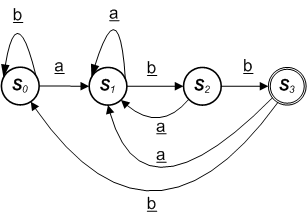
\includegraphics[width=.9\linewidth]{./pic/regularExpressionMatching.png}
\caption{Regular Expression Matching}
\end{figure}

来自 \url{http://leetcode.com/2011/09/regular-expression-matching.html}

\lstset{language=java,label= ,caption= ,numbers=none}
\begin{lstlisting}
bool isMatch(const char *s, const char *p) {  
    if (*p == '\0') return *s == '\0'; 
    if (*(p + 1) != '*') {  
        if (*p == *s || (*p == '.' && *s != '\0'))
            return isMatch(s + 1, p + 1);
        else return false;
    } else { // next char is '*'
        while (*p == *s || (*p == '.' && *s != '\0')) {
            if (isMatch(s, p + 2)) // can optimize
                return true;
            s++;                 // but easier to understand
        }
    }
    return isMatch(s, p + 2);
}
\end{lstlisting}

搜到两种 Java 的解法,改天自己得再好好研究下。。。来自《压栈底的弱渣》

暂时只想出来了递归解法。其实就是自动机的实现原理。

对于两个字符串:string,pattern 有两种情况:

当 pattern[ 1 ] 不为 “*” 的时候(或 pattern 长度为1),直接比较
patter[ 0 ] 和 string[ 0 ] 是否相等。若不等,则直接返回false;若相等,则接着比较他们后面的字符,即跳到自动机的下一个state。

当 pattern[ 1 ] 为 “*” 的时候,情况就稍微复杂一点了。

~ ~ 若 pattern[ 0 ] != string[ 0 ] ,或 string 长度为0时,应跳过 pattern[ 0 ] 和 pattern[ 1 ] 继续比较后面的字符,因为 “*” 为optional symbol。

~ ~ 若 pattern[ 0 ] == string[ 0 ] ,我们既可以跳过 string[ 0 ] ,也可以跳过 pattern[ 0 ] 和 pattern[ 1 ]  。

\lstset{language=java,label= ,caption= ,numbers=none}
\begin{lstlisting}
public boolean isMatch(String s, String p) {
    if (p.length() == 0) return s.length() == 0;
    if (p.length() == 1 || p.charAt(1)!='*') {
        if (s.length() > 0 &&
            (p.charAt(0) == '.' || s.charAt(0) == p.charAt(0)))
            return isMatch(s.substring(1), p.substring(1));
        else return false;
    } else {
        if (s.length() == 0) return isMatch(s, p.substring(2));
        if (p.charAt(0) == '.' || s.charAt(0) == p.charAt(0)) 
            return isMatch(s.substring(1), p) || isMatch(s, p.substring(2));
        else return isMatch(s, p.substring(2));
    }
}
\end{lstlisting}

在Java 1.7以后,String.substring() 这个方法会重新拷贝一个新的字符串,这样在递归过程中内存效率很低, 而且会消耗大量时间用来对象初始化。因而可以考虑在递归的时候传index进去。

改进代码如下:
\lstset{language=java,label= ,caption= ,numbers=none}
\begin{lstlisting}
public boolean isMatchHelper(String s, String p, int is, int ip){
    if (ip == p.length()) return is  ==  s.length();
    if (ip == p.length()-1 || p.charAt(ip + 1)!='*'){ // no *
        if ( is < s.length() &&
             (p.charAt(ip) == '.' || s.charAt(is) == p.charAt(ip)) ) 
            return isMatchHelper(s, p, is + 1, ip + 1); 
        else return false;
    } else {                                          // with *
        if (is == s.length())
            return isMatchHelper(s,p,is,ip + 2);      // empty
        if (p.charAt(ip) == '.' || s.charAt(is) == p.charAt(ip)) //match
            return isMatchHelper(s, p, is + 1, ip)
                || isMatchHelper(s, p, is, ip + 2);  // two choices for continue
        else return isMatchHelper(s, p, is, ip + 2); // not match
    }
}

public boolean isMatch(String s, String p) {
    return isMatchHelper(s, p, 0, 0);
}
\end{lstlisting}

\item 动态规划:
\label{sec-14-3-9-2}

仅次于 Scramble String 的最复杂的动规。。。

思路改天再写,\ldots{} 
\lstset{language=java,label= ,caption= ,numbers=none}
\begin{lstlisting}
public boolean isMatch(String s, String p) {
    if (p.length() == 0 && s.length() == 0) return true;
    if (p.length() == 0 && s.length() > 0) return false;
    int m = s.length();
    int n = p.length();
    boolean [][] dp = new boolean[m + 1][n + 1];
    dp[0][0] = true;
    for (int i = 1; i <= m ; i++)
        dp[i][0] = false;
    for (int i = 1; i <= n ; i++)
        if (i >= 2)
            dp[0][i] = (p.charAt(i - 1) == '*') ? dp[0][i - 2] : false;
    for (int i = 1; i <= m ; i++) {
        for (int j = 1; j <= n ; j++) {
            if (p.charAt(j - 1) == '.')
                dp[i][j] = dp[i - 1][j - 1];
            else if (p.charAt(j - 1) == '*')
                dp[i][j] = ( dp[i][j - 1] || dp[i][j - 2] ||
                             (dp[i - 1][j] &&
                              ((s.charAt(i - 1) == p.charAt(j - 2)  || p.charAt(j - 2) == '.'))) );
            else if (s.charAt(i - 1) == p.charAt(j - 1)) 
                dp[i][j] = dp[i - 1][j - 1];
        }
    }
    return dp[m][n];
}
\end{lstlisting}
\end{enumerate}

\subsection{Wildcard Matching}
\label{sec-14-3-10}
Implement wildcard pattern matching with support for '?' and '*'.
\lstset{language=java,label= ,caption= ,numbers=none}
\begin{lstlisting}
'?' Matches any single character.
'*' Matches any sequence of characters (including the empty sequence).
\end{lstlisting}

The matching should cover the entire input string (not partial).

The function prototype should be:

bool isMatch(const char *s, const char *p)

Some examples:
\lstset{language=java,label= ,caption= ,numbers=none}
\begin{lstlisting}
isMatch("aa","a") → false
isMatch("aa","aa") → true
isMatch("aaa","aa") → false
isMatch("aa", "*") → true
isMatch("aa", "a*") → true
isMatch("ab", "?*") → true
isMatch("aab", "c*a*b") → false
\end{lstlisting}

\textbf{Tags:} Dynamic Programming, Backtracking, Greedy, String

跟上一题很类似。

主要是'*' 的匹配问题。p 每遇到一个'*', 就保留住当前'*' 的坐标和 s 的坐标, 然后 s 从前
往后扫描, 如果不成功, 则 s++, 重新扫描。

除 Scramble String 外最复杂的 DP, 因为 '*' 可以什么也不用配。

\begin{enumerate}
\item 递归版: 时间复杂度 O(n!*m!), 空间复杂度 O(n)
\label{sec-14-3-10-1}

递归版, 会超时, 用于帮助理解题意.

\lstset{language=java,label= ,caption= ,numbers=none}
\begin{lstlisting}
bool isMatch(const char *s, const char *p) {
    if (*p == '*') {
        while (*p == '*') ++p;
        if (*p == '\0') return true;
        while (*s != '\0' && !isMatch(s, p)) ++s;
        return *s != '\0';
    } else if (*p == '\0' || *s == '\0') return *p == *s;
    else if (*p == *s || *p == '?') return isMatch(++s, ++p);
    else return false;
}
\end{lstlisting}

\item 迭代版: 时间复杂度 O(n*m), 空间复杂度 O(1)
\label{sec-14-3-10-2}

\item 动态规划:
\label{sec-14-3-10-3}

直接使用递归会超出内存或者超时,因为递归会重复计算很多相同的内容,可以使用动态规划利用中间结果来避免重复计算。

用 dp[i][j] 表示 s 串的前 i 个字符和 p 串的前 j 个字符是否匹配,则计算

p[i][j] 时,可以根据p的第j个字符分别讨论

p[j-1]为 '*',s可以选择使用这个*,转化为 dp[i-1][j];或者不使用这个'*',变为 dp[i][j-1]。

p[j-1]为 '?',此时p[j-1]必定要匹配s[i-1]。

p[j-1]为普通字符,如果p[j-1]==s[i-1],匹配成功,问题转化为dp[i-1][j-1],否则匹配失败,dp[i][j] = false。
\lstset{language=java,label= ,caption= ,numbers=none}
\begin{lstlisting}
if (p[j-1] == '*') then dp[i][j] = dp[i-1][j] || dp[i][j-1]
if (p[j-1] == '?') then dp[i][j] = dp[i-1][j-1]
if (p[j-1] == s[i-1])   dp[i][j] = dp[i-1][j-1] else dp[i][j]=false//普通字符
\end{lstlisting}
当 i 或 j 为 0 时作为初始化部分,根据定义,应有:

dp[ 0 ][ 0 ] = true。

dp[i][ 0 ] = false,因为有长度的s肯定无法和空串p匹配。

dp[ 0 ][i],只有p[i-1]为*且dp[ 0 ][i-1]为真是才为真。

\lstset{language=java,label= ,caption= ,numbers=none}
\begin{lstlisting}
public boolean isMatch(String s, String p) {
    int minLen = 0;
    for (int i = 0; i < p.length(); i++) 
        if (p.charAt(i) != '*') ++minLen;
    if (s.length() < minLen) return false;
    int m = s.length();
    int n = p.length();
    boolean [][] dp = new boolean[m + 1][n + 1];
    dp[0][0] = true;
    for (int i = 1; i <= m ; i++) 
        dp[i][0] = false;
    for (int i = 1; i <= n ; i++) 
        dp[0][i] = (p.charAt(i - 1) == '*' && dp[0][i - 1]) ? true : false;
    for (int i = 1; i <= m; i++) 
        for (int j = 1; j <= n ; j++) {
            if (p.charAt(j - 1) == '*')  // user * or not
                dp[i][j] = (dp[i - 1][j] || dp[i][j - 1]);
            else if (s.charAt(i - 1) == p.charAt(j - 1) || p.charAt(j - 1) == '?')
                dp[i][j] = dp[i - 1][j - 1];
        }
    return dp[m][n];
}
\end{lstlisting}
\end{enumerate}

\section{others Covered}
\label{sec-14-4}
\begin{itemize}
\item Best Time to Buy and Sell Stock
\ref{sec-13-1-2}
\item Best Time to Buy and Sell Stock II
\ref{sec-13-1-3}
\item Longest Valid Parentheses
\ref{sec-5-3-1}
\item Word Break II
\ref{sec-10-2-1}
\item Maximum Rectangle
\texttt{Maximum Rectangle}
\end{itemize}

\chapter{Two Pointers and Sliding Window}
\label{sec-15}
\section{Easy}
\label{sec-15-1}
\subsection{Valid Palindrome}
\label{sec-15-1-1}
\subsection{Remove Nth Node From End of List}
\label{sec-15-1-2}
\subsection{Remove Element}
\label{sec-15-1-3}
\subsection{Remove Duplicates from Sorted Array}
\label{sec-15-1-4}
\subsection{Merge Sorted Array}
\label{sec-15-1-5}
\subsection{Implement strStr()}
\label{sec-15-1-6}
\section{Medium}
\label{sec-15-2}
\subsection{3Sum}
\label{sec-15-2-1}
\subsection{4Sum}
\label{sec-15-2-2}
\subsection{Container With Most Water}
\label{sec-15-2-3}
\subsection{Remove Duplicates from Sorted Array II}
\label{sec-15-2-4}
\subsection{Partition List}
\label{sec-15-2-5}
\subsection{Two Sum II - Input array is sorted}
\label{sec-15-2-6}
\subsection{Linked List Cycle II}
\label{sec-15-2-7}
\subsection{Longest Substring Without Repeating Characters}
\label{sec-15-2-8}
\subsection{3Sum Closest}
\label{sec-15-2-9}
\subsection{Linked List Cycle}
\label{sec-15-2-10}
\subsection{Sort Colors}
\label{sec-15-2-11}
\subsection{Rotate List}
\label{sec-15-2-12}
\section{Hard}
\label{sec-15-3}
\subsection{Trapping Rain Water}
\label{sec-15-3-1}
\subsection{Longest Substring with At Most Two Distinct Characters}
\label{sec-15-3-2}
\subsection{Substring with Concatenation of All Words}
\label{sec-15-3-3}
\subsection{Minimum Window Substring}
\label{sec-15-3-4}
\chapter{Backtracing and Recursion}
\label{sec-16}
\section{Medium}
\label{sec-16-1}
\subsection{Permutation Sequence}
\label{sec-16-1-1}
The set [1,2,3,…,n] contains a total of n! unique permutations.

By listing and labeling all of the permutations in order, We get the following sequence (ie, for n = 3):
\lstset{language=java,label= ,caption= ,numbers=none}
\begin{lstlisting}
"123"
"132"
"213"
"231"
"312"
"321"
\end{lstlisting}
Given n and k, return the kth permutation sequence.

Note: Given n will be between 1 and 9 inclusive.
\subsection{Gray Code}
\label{sec-16-1-2}
The gray code is a binary numeral system where two successive values differ in only one bit.

Given a non-negative integer n representing the total number of bits in the code, print the sequence of gray code. A gray code sequence must begin with 0.

For example, given n = 2, return [0,1,3,2]. Its gray code sequence is:
\lstset{language=java,label= ,caption= ,numbers=none}
\begin{lstlisting}
00 - 0
01 - 1
11 - 3
10 - 2
\end{lstlisting}
Note:
\begin{itemize}
\item For a given n, a gray code sequence is not uniquely defined.
\item For example, [0,2,3,1] is also a valid gray code sequence according to the above definition.
\item For now, the judge is able to judge based on one instance of gray code sequence. Sorry about that.
\end{itemize}

格雷码 (Gray Code) 的定义请参考 wikipedia \url{http://en.wikipedia.org/wiki/Gray_code}。

自然二进制码转换为格雷码:g 0 = b 0 , g i = b i ⊕ b i−1

保留自然二进制码的最高位作为格雷码的最高位,格雷码次高位为二进制码的高位与次高位异或,其余各位与次高位的求法类似。例如,将自然二进制码 1001,转换为格雷码的过程是:保留最高位;然后将第 1 位的 1 和第 2 位的 0 异或,得到 1,作为格雷码的第 2 位;将第 2 位的 0 和第 3 位的 0 异或,得到 0,作为格雷码的第 3 位;将第 3 位的 0 和第 4 位的 1 异或,得到 1,作为格雷码的第 4 位,最终,格雷码为 1101。

格雷码转换为自然二进制码:b 0 = g 0 , b i = g i ⊕ b i−1

保留格雷码的最高位作为自然二进制码的最高位,次高位为自然二进制高位与格雷码次高位异或,其余各位与次高位的求法类似。例如,将格雷码 1000 转换为自然二进制码的过程是:保留最高位 1,作为自然二进制码的最高位;然后将自然二进制码的第 1 位 1 和格雷码的第 2 位 0 异或,得到1,作为自然二进制码的第 2 位;将自然二进制码的第 2 位 1 和格雷码的第 3 位 0 异或,得到 1,作为自然二进制码的第 3 位;将自然二进制码的第 3 位 1 和格雷码的第 4 位 0 异或,得到 1,作为自然二进制码的第 4 位,最终,自然二进制码为 1111。

格雷码有数学公式,整数 n 的格雷码是 n ⊕ (n/2)。

这题要求生成 n 比特的所有格雷码。

最简单的方法,利用数学公式,对从 0 ∼ 2 n − 1 的所有整数,转化为格雷码。

n 比特的格雷码,可以递归地从 n − 1 比特的格雷码生成。如图 §2-5所示。

\begin{figure}[htb]
\centering
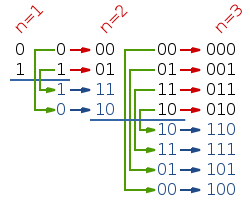
\includegraphics[width=.9\linewidth]{./pic/grayCode.png}
\caption{Gray Code}
\end{figure}

\begin{figure}[htb]
\centering
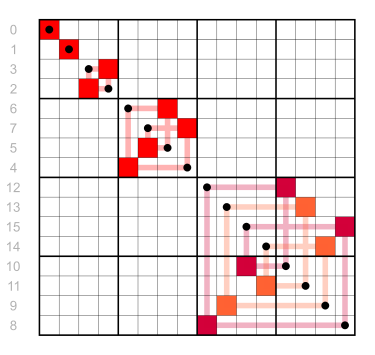
\includegraphics[width=.9\linewidth]{./pic/grayCode2.png}
\caption{Gray Code 2}
\end{figure}

\section{Hard}
\label{sec-16-2}
\subsection{Regular Expression Matching}
\label{sec-16-2-1}
Implement regular expression matching with support for '.' and '*'.
\begin{itemize}
\item '.' Matches any single character.
\item '*' Matches zero or more of the preceding element.
\end{itemize}

The matching should cover the entire input string (not partial).

The function prototype should be:

bool isMatch(const char *s, const char *p)

Some examples:
\lstset{language=java,label= ,caption= ,numbers=none}
\begin{lstlisting}
isMatch("aa","a") → false
isMatch("aa","aa") → true
isMatch("aaa","aa") → false
isMatch("aa", "a*") → true
isMatch("aa", ".*") → true
isMatch("ab", ".*") → true
isMatch("aab", "c*a*b") → true
\end{lstlisting}
\textbf{Tags:} Dynamic Programming, Backtracking, String
\subsection{Wild Card Matching}
\label{sec-16-2-2}
Implement wildcard pattern matching with support for '?' and '*'.
\begin{itemize}
\item '?' Matches any single character.
\item '*' Matches any sequence of characters (including the empty sequence).
\end{itemize}

The matching should cover the entire input string (not partial).

The function prototype should be:

bool isMatch(const char *s, const char *p)

Some examples:
\lstset{language=java,label= ,caption= ,numbers=none}
\begin{lstlisting}
isMatch("aa","a") → false
isMatch("aa","aa") → true
isMatch("aaa","aa") → false
isMatch("aa", "*") → true
isMatch("aa", "a*") → true
isMatch("ab", "?*") → true
isMatch("aab", "c*a*b") → false
\end{lstlisting}
\textbf{Tags:} Dynamic Programming, Backtracking, Greedy, String
\subsection{Word Break II}
\label{sec-16-2-3}
Given a string s and a dictionary of words dict, add spaces in s to construct a sentence where each word is a valid dictionary word.

Return all such possible sentences.

For example, given
\lstset{language=java,label= ,caption= ,numbers=none}
\begin{lstlisting}
s = "catsanddog",
dict = ["cat", "cats", "and", "sand", "dog"].

A solution is ["cats and dog", "cat sand dog"].
\end{lstlisting}
\textbf{Tags:} Dynamic Programming Backtracking
\section{other Covered}
\label{sec-16-3}
\begin{itemize}
\item Subsets
\ref{sec-9-1-1}
\item Subsets II
\ref{sec-9-1-2}
\item Combinationas
\ref{sec-9-1-4}
\item Letter Combinationas of Phone Number
\ref{sec-9-1-5}
\item Permutation
\ref{sec-9-1-3}
\item Permutation II
\ref{sec-9-2-1}
\item Palindrome Partitioning 
\ref{sec-11-1-1}
\item Restore IP Addresses
\ref{sec-11-1-2}
\item N-Queens 
\ref{sec-11-2-1}
\item N-Queens II
\ref{sec-11-2-2}
\item Combination Sum
\ref{sec-11-1-4}
\item Combination Sum II
\ref{sec-11-1-5}
\item Generate Parentheses
\ref{sec-11-1-3}
\item Sudoku Solver
\ref{sec-6-3-3}
\item Word Search
\ref{sec-11-2-4}
\item Word Ladder II
\ref{sec-10-2-1}
\end{itemize}
\chapter{Bit Manipulation}
\label{sec-17}
\section{Easy}
\label{sec-17-1}
\subsection{Majority Element}
\label{sec-17-1-1}
Given an array of size n, find the majority element. The majority element is the element that appears more than ⌊ n/2 ⌋ times.

You may assume that the array is non-empty and the majority element always exist in the array.

Credits:

Special thanks to @ts for adding this problem and creating all test cases.

\textbf{Tags:} Divide and Conquer, Array, Bit Manipulation

\section{Medium}
\label{sec-17-2}
\subsection{Subsets: Bit Manipulation}
\label{sec-17-2-1}
Given a set of distinct integers, S, return all possible subsets.

Note:
\begin{itemize}
\item Elements in a subset must be in non-descending order.
\item The solution set must not contain duplicate subsets.
\end{itemize}
For example,
If S = [1,2,3], a solution is:
\lstset{language=java,label= ,caption= ,numbers=none}
\begin{lstlisting}
[
  [3],
  [1],
  [2],
  [1,2,3],
  [1,3],
  [2,3],
  [1,2],
  []
]
\end{lstlisting}
\textbf{Tags:} Array Backtracking, Bit Manipulation
\subsection{Single Number}
\label{sec-17-2-2}
Given an array of integers, every element appears twice except for one. Find that single one.

Note:

Your algorithm should have a linear runtime complexity. Could you implement it without using extra memory?

\textbf{Tags:} Hash Table, Bit Manipulation

\subsection{Single Number II}
\label{sec-17-2-3}
Given an array of integers, every element appears three times except for one. Find that single one.

Note:

Your algorithm should have a linear runtime complexity. Could you implement it without using extra memory?

\chapter{图 Graphics}
\label{sec-18}
\section{Medium}
\label{sec-18-1}
\subsection{Clone Graph}
\label{sec-18-1-1}
Clone an undirected graph. Each node in the graph contains a label and a list of its neighbors.

OJ's undirected graph serialization:

Nodes are labeled uniquely.

We use \# as a separator for each node, and , as a separator for node label and each neighbor of the node.

As an example, consider the serialized graph \{0,1,2\#1,2\#2,2\}.

The graph has a total of three nodes, and therefore contains three parts as separated by \#.

\begin{enumerate}
\item First node is labeled as 0. Connect node 0 to both nodes 1 and 2.
\item Second node is labeled as 1. Connect node 1 to node 2.
\item Third node is labeled as 2. Connect node 2 to node 2 (itself), thus forming a self-cycle.
\end{enumerate}

Visually, the graph looks like the following:
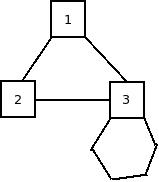
\includegraphics[width=.9\linewidth]{./pic/clonegraph.jpg}

\begin{enumerate}
\item 分析: 广度优先遍历或深度优先遍历都可以
\label{sec-18-1-1-1}
\item DFS: 时间复杂度O(n), 空间复杂度O(n)
\label{sec-18-1-1-2}
\lstset{language=java,label= ,caption= ,numbers=none}
\begin{lstlisting}
/**
 * Definition for undirected graph.
 * class UndirectedGraphNode {
 *     int label;
 *     List<UndirectedGraphNode> neighbors;
 *     UndirectedGraphNode(int x) { label = x; neighbors = new ArrayList<UndirectedGraphNode>(); }
 * };
 */
public UndirectedGraphNode cloneGraph(UndirectedGraphNode node) {
    if (node == null) return null;
    UndirectedGraphNode res = new UndirectedGraphNode(node.label);  // result head
    if (node.neighbors == null || node.neighbors.size() == 0) return res;

    Map<UndirectedGraphNode, UndirectedGraphNode> map = new HashMap<UndirectedGraphNode, UndirectedGraphNode>();
    Queue<UndirectedGraphNode> q = new LinkedList<UndirectedGraphNode>();
    q.add(node);                      // added first node, need add its all Neighbors as well
    map.put(node, res);

    List<UndirectedGraphNode> curNbr = new ArrayList<UndirectedGraphNode>();
    UndirectedGraphNode curr = null;
    while (!q.isEmpty()) {
        curr = q.poll();
        curNbr = curr.neighbors;                   // ori
        for (UndirectedGraphNode aNbr : curNbr) {  // for build connection among copies
            if (!map.containsKey(aNbr)) {
                UndirectedGraphNode acpNbr = new UndirectedGraphNode(aNbr.label);
                map.put(aNbr, acpNbr);
                map.get(curr).neighbors.add(acpNbr);
                q.add(aNbr);
            } else
                map.get(curr).neighbors.add(map.get(aNbr));                        
        }
    }
    return res;
}
\end{lstlisting}
\item BFS:
\label{sec-18-1-1-3}
\end{enumerate}
\subsection{Check whether the graph is bigraph}
\label{sec-18-1-2}
\begin{enumerate}
\item Topological Sort
\label{sec-18-1-2-1}
Topological sorting for Directed Acyclic Graph (DAG) is a linear
ordering of vertices such that for every directed edge uv, vertex u
comes before v in the ordering. Topological Sorting for a graph is not
possible if the graph is not a DAG.

For example, a topological sorting of the following graph is “5 4 2 3
1 0″. There can be more than one topological sorting for a graph. For
example, another topological sorting of the following graph is “4 5 2
3 1 0″. The first vertex in topological sorting is always a vertex
with in-degree as 0 (a vertex with no in-coming edges).
\begin{figure}[htb]
\centering
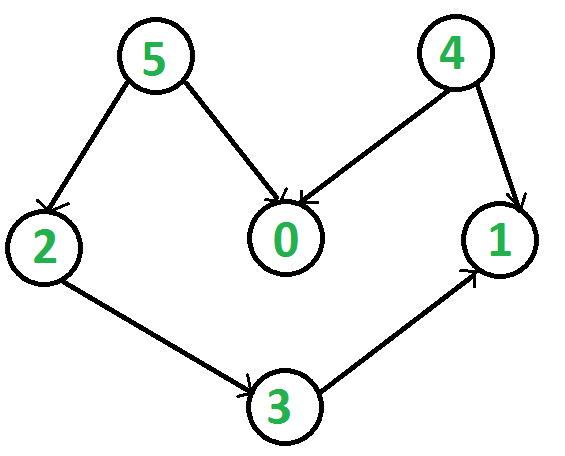
\includegraphics[width=.9\linewidth]{./pic/topologicalSorting.png}
\caption{Topological Sorting}
\end{figure}
\item Topological Sorting vs Depth First Traversal (DFS):
\label{sec-18-1-2-2}
In DFS, we print a vertex and then recursively call DFS for its adjacent vertices. In topological sorting, we need to print a vertex before its adjacent vertices. For example, in the given graph, the vertex ‘5’ should be printed before vertex ‘0’, but unlike DFS, the vertex ‘4’ should also be printed before vertex ‘0’. So Topological sorting is different from DFS. For example, a DFS of the above graph is “5 2 3 1 0 4″, but it is not a topological sorting.
\item Algorithm to find Topological Sorting:
\label{sec-18-1-2-3}
We recommend to first see implementation of DFS here. We can modify DFS to find Topological Sorting of a graph. In DFS, we start from a vertex, we first print it and then recursively call DFS for its adjacent vertices. In topological sorting, we use a temporary stack. We don’t print the vertex immediately, we first recursively call topological sorting for all its adjacent vertices, then push it to a stack. Finally, print contents of stack. Note that a vertex is pushed to stack only when all of its adjacent vertices (and their adjacent vertices and so on) are already in stack.
\end{enumerate}
\section{other Covered}
\label{sec-18-2}
\begin{itemize}
\item Word Ladder \ref{sec-10-1-2}
\item Word Ladder II
\end{itemize}
\ref{sec-10-2-1}

\chapter{Data Structure}
\label{sec-19}
\section{Easy}
\label{sec-19-1}
\subsection{Two Sum III}
\label{sec-19-1-1}
Design and implement a TwoSum class. It should support the following operations: add and find.
\begin{itemize}
\item add - Add the number to an internal data structure.
\item find - Find if there exists any pair of numbers which sum is equal to the value.
\end{itemize}
For example,
\lstset{language=java,label= ,caption= ,numbers=none}
\begin{lstlisting}
add(1); add(3); add(5);
find(4) -> true
find(7) -> false
\end{lstlisting}
\textbf{Tags:} Hash Table, Data Structure

\subsection{Min Stack}
\label{sec-19-1-2}
Design a stack that supports push, pop, top, and retrieving the minimum element in constant time.
\begin{itemize}
\item push(x) -- Push element x onto stack.
\item pop() -- Removes the element on top of the stack.
\item top() -- Get the top element.
\item getMin() -- Retrieve the minimum element in the stack.
\textbf{Tags:} Stack Data Structure
\end{itemize}
\lstset{language=java,label= ,caption= ,numbers=none}
\begin{lstlisting}
public static class MinStack {
    Stack<Integer> stack = new Stack<Integer>();
    Stack<Integer> minStack = new Stack<Integer>();
    public void push(int x) {
        stack.push(x);
        if (minStack.isEmpty() || x <= minStack.peek()) {
            minStack.push(x);
        }
    }

    public void pop() { // java boxing & unboxing, container, object specific methods
        if (stack.peek().intValue() == minStack.peek().intValue()) 
            minStack.pop();
        stack.pop();
    }

    public int top() {
        return stack.peek();
    }

    public int getMin() {
        if (!minStack.isEmpty()) return minStack.peek();
        else return -1;
    }
}
\end{lstlisting}
\section{Hard}
\label{sec-19-2}
\subsection{LRU Cache}
\label{sec-19-2-1}
Design and implement a data structure for Least Recently Used (LRU) cache. It should support the following operations: get and set.
\begin{itemize}
\item get(key) - Get the value (will always be positive) of the key if the key exists in the cache, otherwise return -1.
\item set(key, value) - Set or insert the value if the key is not already
present. When the cache reached its capacity, it should invalidate
the least recently used item before inserting a new item.
\end{itemize}
\lstset{language=java,label= ,caption= ,numbers=none}
\begin{lstlisting}
public static class LRUCache {
    public class Node {
        int key;
        int value;
        Node prev;
        Node next;
        public Node(int x, int y){
            key = x;
            value = y;
        }
    }

    private HashMap<Integer, Node> hash;
    private int cap;
    private int number;
    Node head;
    Node tail;
    public LRUCache(int capacity) {
        cap = capacity;
        number = 0;
        head = new Node(-1, -1);
        head.prev = null;
        head.next = null;
        tail = head;
        hash = new HashMap<Integer, Node>(capacity); // so I can restrict a size !!
    }

    public int get(int key) {
        Node res = hash.get(new Integer(key)); // don't understand here
        if (res != null) {
            refresh(res);   // update usage frequence
            return res.value;
        } else return -1;
        /*
          if (hash.containsKey(key)) {
          //Node res = hash.get(new Integer(key)); // don't understand here
          Node res = hash.get(key);
          refresh(res);   // update usage frequence
          return res.value;
          } else {
          return -1;
          }
        */
    }

    // so still, must maintain a doubly-linked list to order usage frequency
    public  void refresh(Node tmp) {
        if (tmp == head.next) return; // it's head already

        Node temp = head.next;  // head node in the hash
        Node prevNode = tmp.prev;
        Node nextNode = tmp.next;
        // set to be most recently used~~ move the tmp node to be head.next, connections
        head.next = tmp;  
        tmp.prev = head;
        tmp.next = temp;
        temp.prev = tmp;
        prevNode.next = nextNode;
        if (nextNode != null) 
            nextNode.prev = prevNode;
        else tail = prevNode;   // remember tail as well 
    }

    public void set(int key, int value) {
        Node res = hash.get(new Integer(key));
        if (res != null) {
            refresh(res);
            res.value = value;
        } else {
            //if (!hash.containsKey(key)) { // another way of detecting existing
            Node prevNode = new Node(key, value); 
            Node temp;
            if (number == cap) { // remove tail;
                temp = tail.prev;
                hash.remove(tail.key);      // remember to remove from hash too !!!
                if (temp != null) {
                    temp.next = null;
                }
                tail.prev = null;
                tail = temp;
                number--;
            }
            // add to tail first
            tail.next = prevNode;
            prevNode.prev = tail;
            tail = prevNode;
            refresh(prevNode);
            hash.put(key, prevNode); 
            number++;  // count node numbers
        }
    }
}
\end{lstlisting}
\chapter{细节实现题}
\label{sec-20}
\section{Medium}
\label{sec-20-1}
\subsection{Pascal's Triangle}
\label{sec-20-1-1}
\subsection{Pascal's Triangle II}
\label{sec-20-1-2}
\subsection{Two Sum}
\label{sec-20-1-3}
\subsection{Two Sum II - Input array is sorted}
\label{sec-20-1-4}
\subsection{Insert Interval}
\label{sec-20-1-5}
\subsection{Merge Intervals}
\label{sec-20-1-6}
\subsection{Spiral Matrix}
\label{sec-20-1-7}
\subsection{Spiral Matrix II}
\label{sec-20-1-8}
\subsection{Multiply Strings}
\label{sec-20-1-9}
\subsection{Substring with Concatenation of All Words}
\label{sec-20-1-10}
\subsection{ZigZag Conversion}
\label{sec-20-1-11}
\subsection{Text Justification}
\label{sec-20-1-12}
\section{other Covered}
\label{sec-20-2}
\begin{itemize}
\item Majority Element
\item Container With Most Water
\item Minimum Path Sum
\item Missing Ranges
\item Find Minimum in Rotated Sorted Array
\item Triangle
\item Find Peak Element
\item Find Minimum in Rotated Sorted Array II
\item Jump Game II
\item Word Ladder II
\end{itemize}

\chapter{Math}
\label{sec-21}
\section{Easy}
\label{sec-21-1}
\subsection{Add Binary}
\label{sec-21-1-1}
\subsection{String to Integer (atoi)}
\label{sec-21-1-2}
\subsection{Palindrome Number}
\label{sec-21-1-3}
\subsection{Factorial Trailing Zeroes}
\label{sec-21-1-4}
\subsection{Excel Sheet Column Title}
\label{sec-21-1-5}
\subsection{Excel Sheet Column Number}
\label{sec-21-1-6}
\subsection{Reverse Integer}
\label{sec-21-1-7}
\section{Medium}
\label{sec-21-2}
\subsection{Multiply Strings}
\label{sec-21-2-1}
\subsection{Divide Two Integers}
\label{sec-21-2-2}
\subsection{Fraction to Recurring Decimal}
\label{sec-21-2-3}
\subsection{Permutation Sequence}
\label{sec-21-2-4}
\subsection{Next Permutation}
\label{sec-21-2-5}
Implement next permutation, which rearranges numbers into the lexicographically next greater permutation of numbers.

If such arrangement is not possible, it must rearrange it as the lowest possible order (ie, sorted in ascending order).

The replacement must be in-place, do not allocate extra memory.

Here are some examples. Inputs are in the left-hand column and its
corresponding outputs are in the right-hand column.
\lstset{language=java,label= ,caption= ,numbers=none}
\begin{lstlisting}
1,2,3 → 1,3,2
3,2,1 → 1,2,3
1,1,5 → 1,5,1
\end{lstlisting}
\section{Hard}
\label{sec-21-3}
\subsection{Valid Number}
\label{sec-21-3-1}
\subsection{Max Points on a Line}
\label{sec-21-3-2}
\section{other Covered}
\label{sec-21-4}
\begin{itemize}
\item Plus One
\ref{sec-1-1-3}
\item Roman to Integers
\texttt{Roman to Integers}
\item Integer to Roman
\ref{sec-2-2-2}
\item Pow(x, n)
\ref{sec-12-1-1}
\item Sqrt(x)
\ref{sec-12-1-2}
\end{itemize}
% Emacs 24.3.1 (Org mode 8.2.7c)
\end{document}